%============================================================
% ChinaVIS-1-I
% - 在仓库根目录 /workspace 下，完整编译命令是：
%   cd /workspace/files/competition && xelatex -interaction=nonstopmode -halt-on-error papre.tex
% - 想交叉引用和分页更稳定，一般连跑两次：
%   cd /workspace/files/competition && xelatex -interaction=nonstopmode -halt-on-error papre.tex && xelatex -interaction=nonstopmode -halt-on-error papre.tex
%============================================================

% !TEX program = xelatex
\documentclass[12pt, a4paper]{article}

\usepackage[UTF8]{ctex}
\usepackage{fontspec}
\usepackage{amssymb}
\usepackage{amsmath}
\usepackage{textcomp}
\usepackage{graphicx}
\usepackage{float}
\usepackage{caption}
\usepackage{enumitem}
\usepackage{array}
\usepackage{booktabs}
\usepackage{hyperref}
\captionsetup{labelformat=empty}
\usepackage[
  top=3.6cm, bottom=3.6cm,
  left=3.17cm, right=3.17cm
]{geometry}
\usepackage{setspace}

% ===== 字体 =====
% ctex 默认 Fandol 字体集（宋体/黑体/楷体/仿宋），英文默认 Latin Modern
% 等宽字体用于英文副标题
\newfontfamily\ttmono{Latin Modern Mono}

% 简单下划线
\newcommand{\ul}[1]{\underline{#1}}
\newcolumntype{L}[1]{>{\raggedright\arraybackslash}p{#1}}
\newcolumntype{C}[1]{>{\centering\arraybackslash}p{#1}}

\setlength{\parindent}{0pt}
\setlength{\parskip}{0pt}
\pagestyle{plain}
\setstretch{1.0}

\begin{document}
\pagenumbering{gobble}
\thispagestyle{empty}

%============================================================
% 标题区（全部居中）
%============================================================
\begin{center}

% 行1：主标题
{\fontsize{20bp}{26bp}\selectfont\bfseries
2026年第十三届中国可视化与可视分析大会}

\vspace{10pt}

% 行2：副标题
{\fontsize{20bp}{26bp}\selectfont\bfseries
数据可视化竞赛\enspace 赛道1-I}

\vspace{11pt}

% 行3：英文副标题
{\fontsize{13bp}{19bp}\ttmono\bfseries
(ChinaVis Data Challenge 2026 -- mini challenge 1-I)}

\vspace{11pt}

% 行4："答　卷"
{\fontsize{20bp}{26bp}\selectfont\bfseries
答\quad 卷}

\end{center}

%============================================================
% 标题区与信息区留白
%============================================================
\vspace{2.0cm}

%============================================================
% 信息区
%============================================================

{\fontsize{13bp}{19bp}\heiti 参赛队名称：中南大学-牛晨勋-赛道1-I}

\vspace{28pt}

{\fontsize{13bp}{19bp}\heiti 团队成员：牛晨勋，中南大学，8208231403@csu.edu.cn，队长}

\vspace{16pt}
{\fontsize{13bp}{19bp}\heiti \phantom{团队成员：}雷远智，中南大学，2891455519@qq.com}

\vspace{16pt}
{\fontsize{13bp}{19bp}\heiti \phantom{团队成员：}陈迪文，中南大学，2977893713@qq.com}

\vspace{16pt}
{\fontsize{13bp}{19bp}\heiti \phantom{团队成员：}刘耀徽，中南大学，3384956918@qq.com}

\vspace{16pt}
{\fontsize{13bp}{19bp}\heiti \phantom{团队成员：}李佳明，中南大学，2893523542@qq.com}

\vspace{16pt}
{\fontsize{13bp}{19bp}\heiti \phantom{团队成员：}周芳芳，中南大学，zff@csu.edu.cn}

\vspace{28pt}

{\fontsize{13bp}{19bp}\heiti 团队成员是否与报名表一致（是或否）：是}

\vspace{28pt}

{\fontsize{13bp}{19bp}\heiti 是否学生队（是或否）：是}

\vspace{28pt}

{\fontsize{13bp}{19bp}\heiti 使用的分析工具或开发工具：React，D3.js，Three.js，ECharts，Python}

\vspace{28pt}

{\fontsize{13bp}{19bp}\heiti 共计耗费时间（人天）：40人天}

\vspace{28pt}

{\fontsize{13bp}{19bp}\heiti 本次比赛结束后，我们是否可以在网络上公布该答卷与视频（是或否）：是}

\vspace{2.0cm}

%============================================================
% 正文区
%============================================================

\newpage
\pagenumbering{arabic}
\setcounter{page}{1}
\setlength{\parindent}{2em}
\setstretch{1.15}

% ============================================================
% 0. 系统概览
% ============================================================

{\fontsize{14bp}{22bp}\heiti\bfseries 0、系统概览：梨园万象——京剧剧本多维可视分析系统}

% \vspace{8pt}

\vspace{3pt}

{\fontsize{12bp}{20bp}\kaishu
我们面向 1{,}473 部跨来源、跨流派京剧剧本，构建了“梨园万象——京剧剧本多维可视分析系统”。系统整体采用“数据层—分析层—可视层”三层架构：数据层负责整合跨来源剧本原始文本、角色信息和场景内容，并完成结构化存储；分析层围绕角色行当、关系网络、主题结构、叙事节奏和综合关联五个维度提取统计结果与比较指标；可视层则由总览页与五个任务页组成，用来承接全局概览、跨剧本比较和单剧验证三类分析过程（图0.1）。
}

% ================= 图0.1：系统架构图 =================
% 文件存放位置：Image/system-arch.png
% 图片内容：系统的数据层—分析层—可视层架构，突出“多源数据整合—离线分析建模—前端交互展示”的整体链路
% 截图要求：保留完整架构层级、主要数据流向和核心模块名称；尽量使用高分辨率位图，避免文字发虚
%
\begin{figure}[H]
\centering
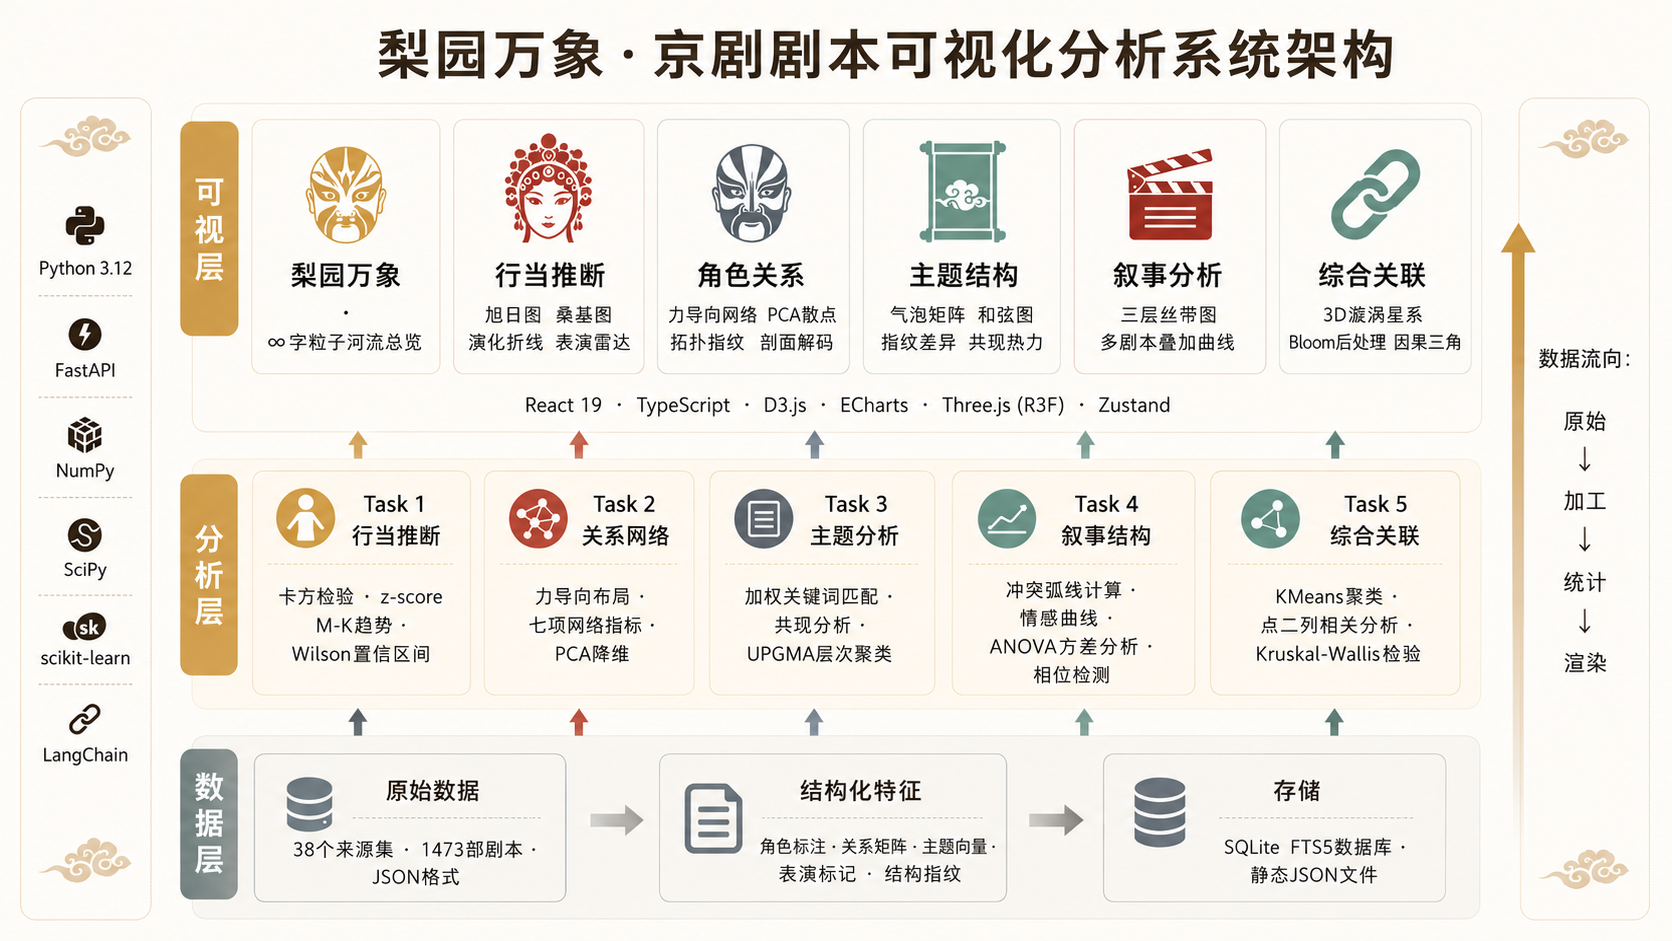
\includegraphics[width=0.85\textwidth]{Image/system-arch.png}
\caption{图0.1 梨园万象系统架构图。}
\end{figure}

% ================= 图0.2：总览页 + 综合页拼图 =================
% 文件存放位置：Image/Overview.png + Image/Task5.png
% 图片内容：左图为总览页，右图为任务五“梨园星图”页面；左图突出全局入口、科普入口与编辑出版年代格局，右图突出星图主视图、因果分析侧栏与结构原型筛选
% 使用方法：图片准备好后，取消下方 figure 注释即可
% 截图要求：两张图都要放大到可读状态，保留主标题、核心图表和关键交互入口；不要截过多空白边缘
%
\begin{figure}[H]
\centering
\begin{minipage}[t]{0.50\textwidth}
  \centering
  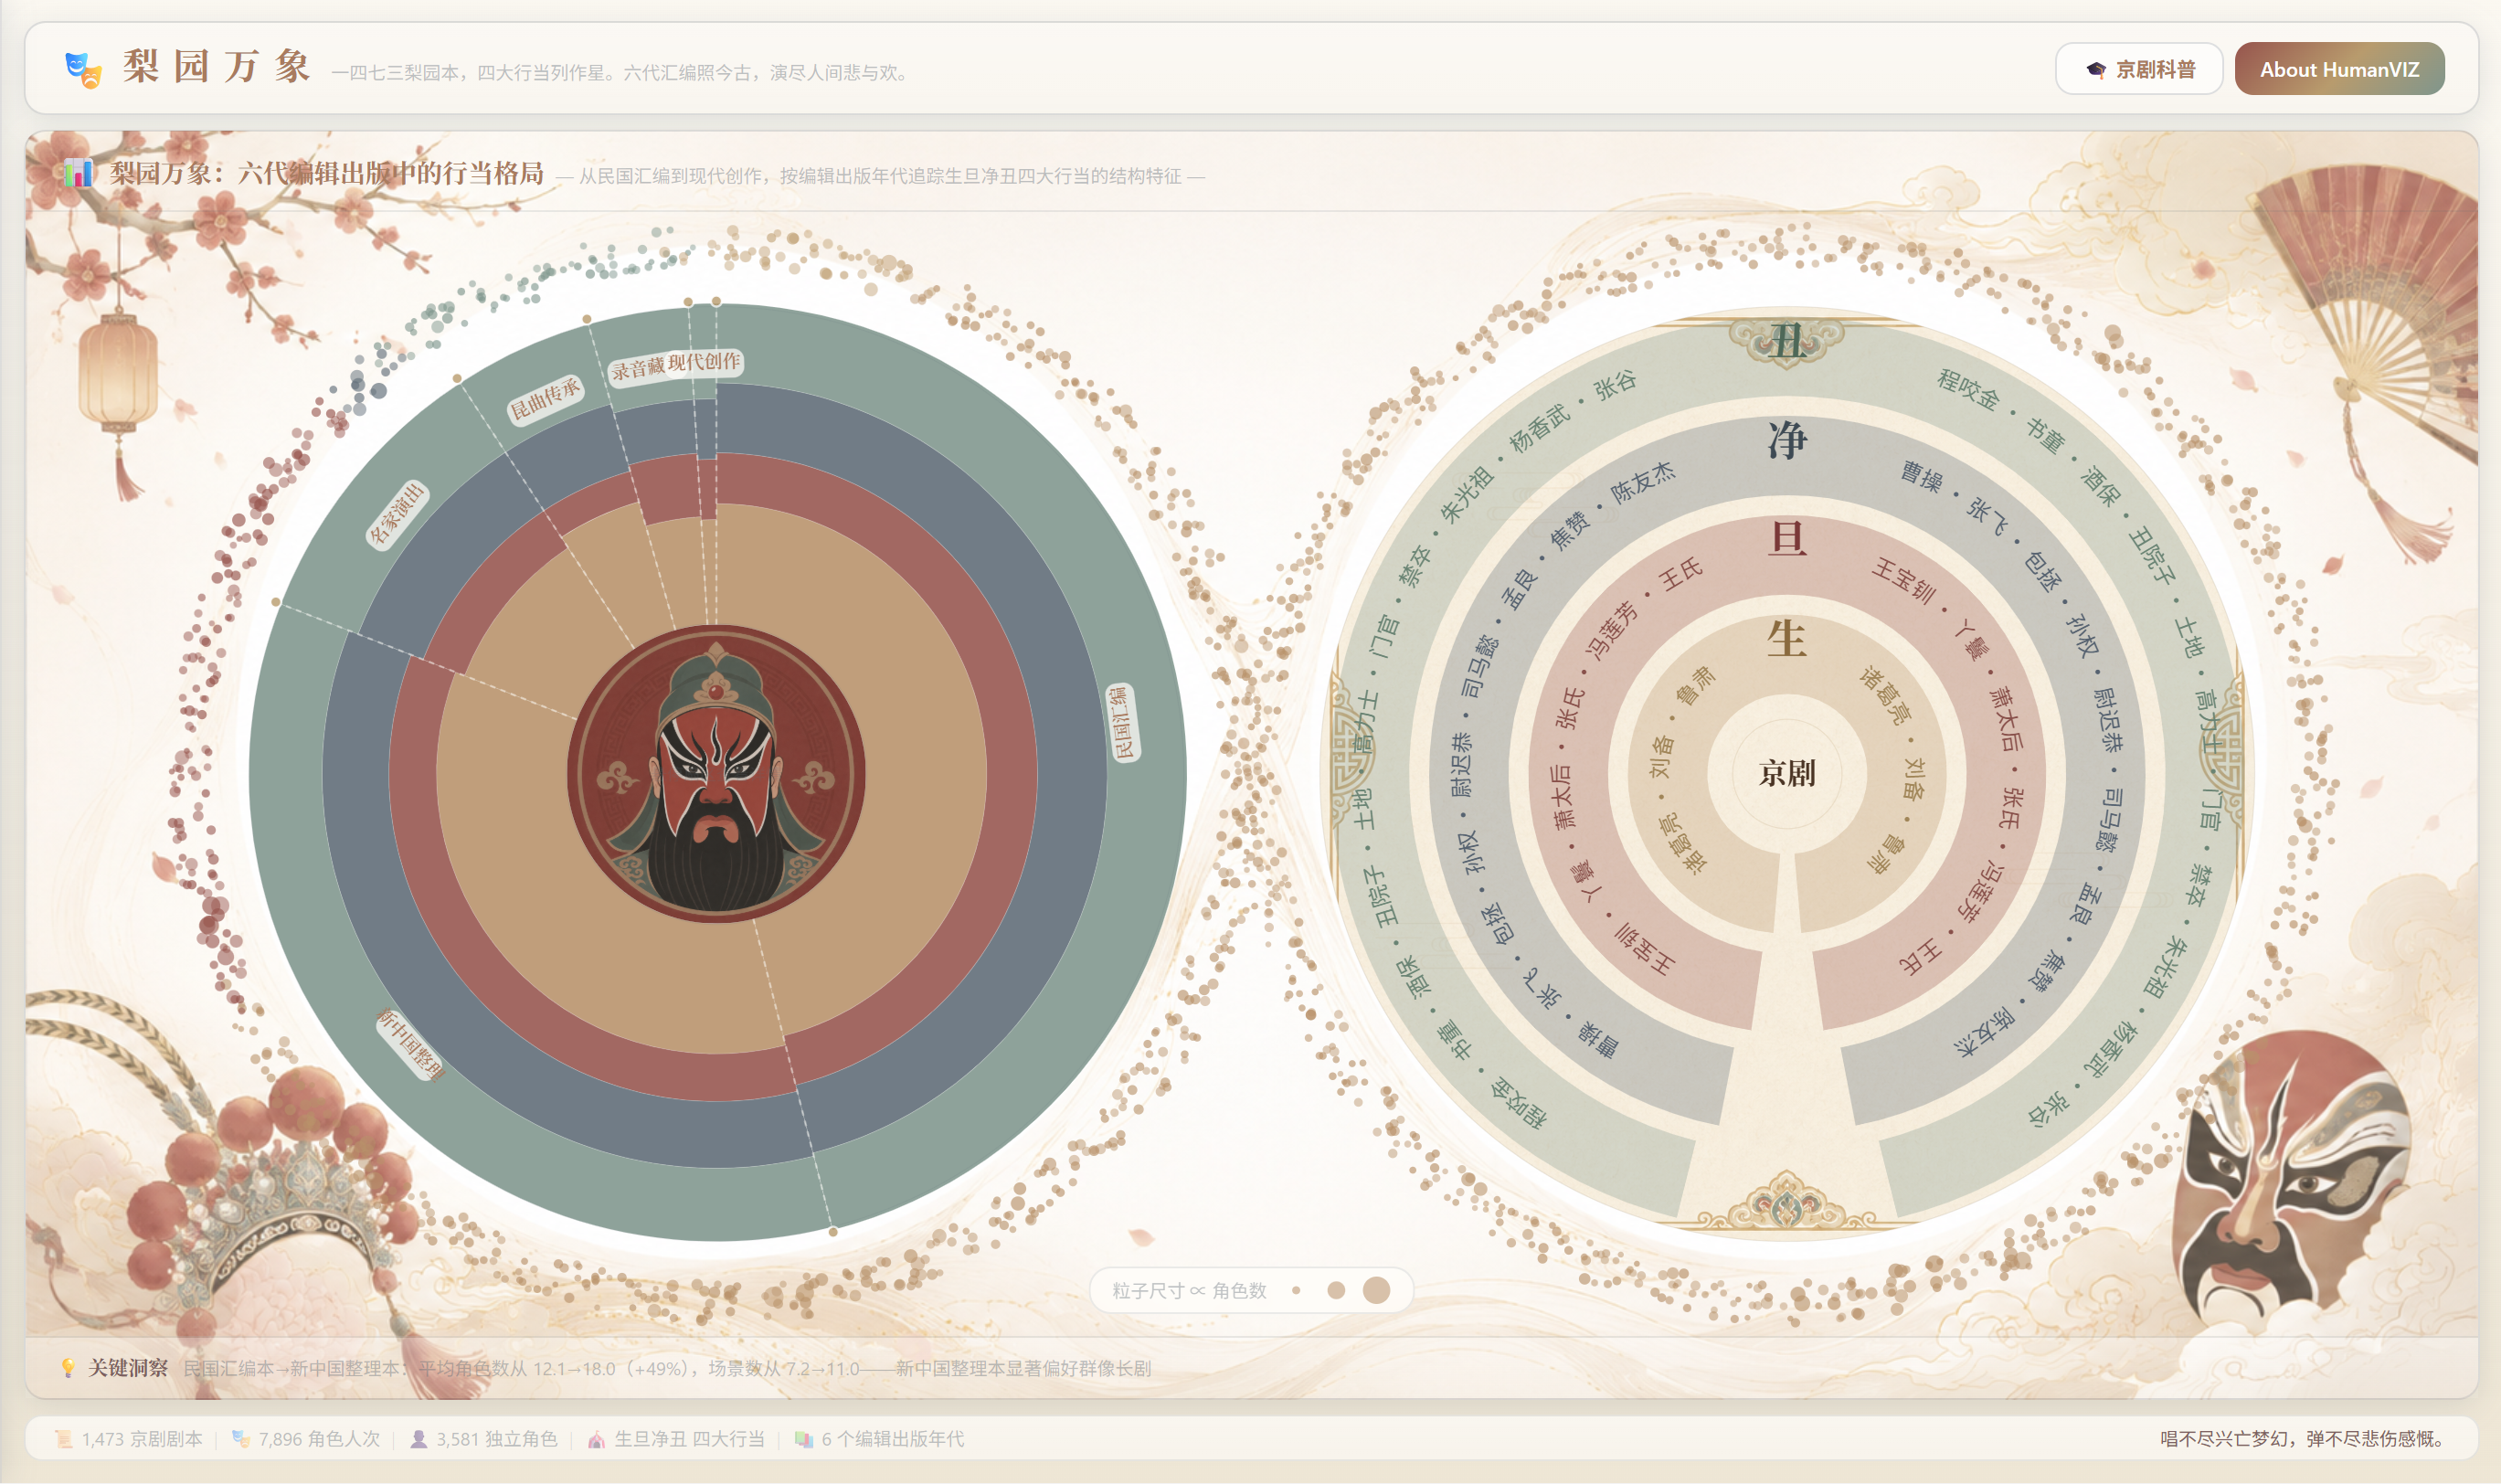
\includegraphics[width=\textwidth]{Image/Overview.png}
  % \caption*{A. 总览页}
\end{minipage}\hfill
\begin{minipage}[t]{0.50\textwidth}
  \centering
  \includegraphics[width=\textwidth]{Image/Task5.png}
  % \caption*{B. 综合分析界面}
\end{minipage}
\caption{图0.2 梨园万象系统总览与综合分析页面。}
\end{figure}

{\fontsize{12bp}{20bp}\kaishu
系统首先呈现的是两个核心页面（图0.2）：
\begin{itemize}[leftmargin=2.2em,itemsep=2pt,topsep=2pt]
\item \textbf{A. 总览页面（左）}：以∞形长河为骨架，将 1{,}473 部剧本按六类编辑出版来源铺展成流动的行当格局。剧本沿河而下，来源与年代也随之舒展开来，像一卷徐徐展开的戏谱；页面右上方设京剧科普入口，底部汇总剧本总数、角色规模与年代分布，也为后续多维分析拉开了序幕。
\item \textbf{B. 综合分析界面（右）}：以梨园星图为主视图，1{,}473 部剧本在此重新汇聚，联动角色关系、主题结构与叙事结构的三角因果分析，支持原型筛选与单剧详情查看。角色、主题与叙事在星图中彼此牵引，也让前面逐步展开的分析在这里收拢成一片更完整的梨园宇宙。
\end{itemize}
}

% ================= 图0.3：任务1-4拼图 =================
% 文件存放位置：Image/Task1.png + Image/Task2.png + Image/Task3.png + Image/Task4.png
% 图片内容：2×2 拼图，依次展示任务1行当推断、任务2角色关系、任务3主题比较、任务4叙事结构四个页面的中央主视图
% 使用方法：图片准备好后，取消下方 figure 注释即可
% 截图要求：每个小图只保留中央主图、标题和关键图例；尽量裁掉侧栏、说明文字与页面边缘装饰，保证四个模块在 PDF 中仍然清晰可读
%
% \vspace{3pt}

\begin{figure}[H]
\centering
\begin{minipage}[t]{0.50\textwidth}
  \centering
  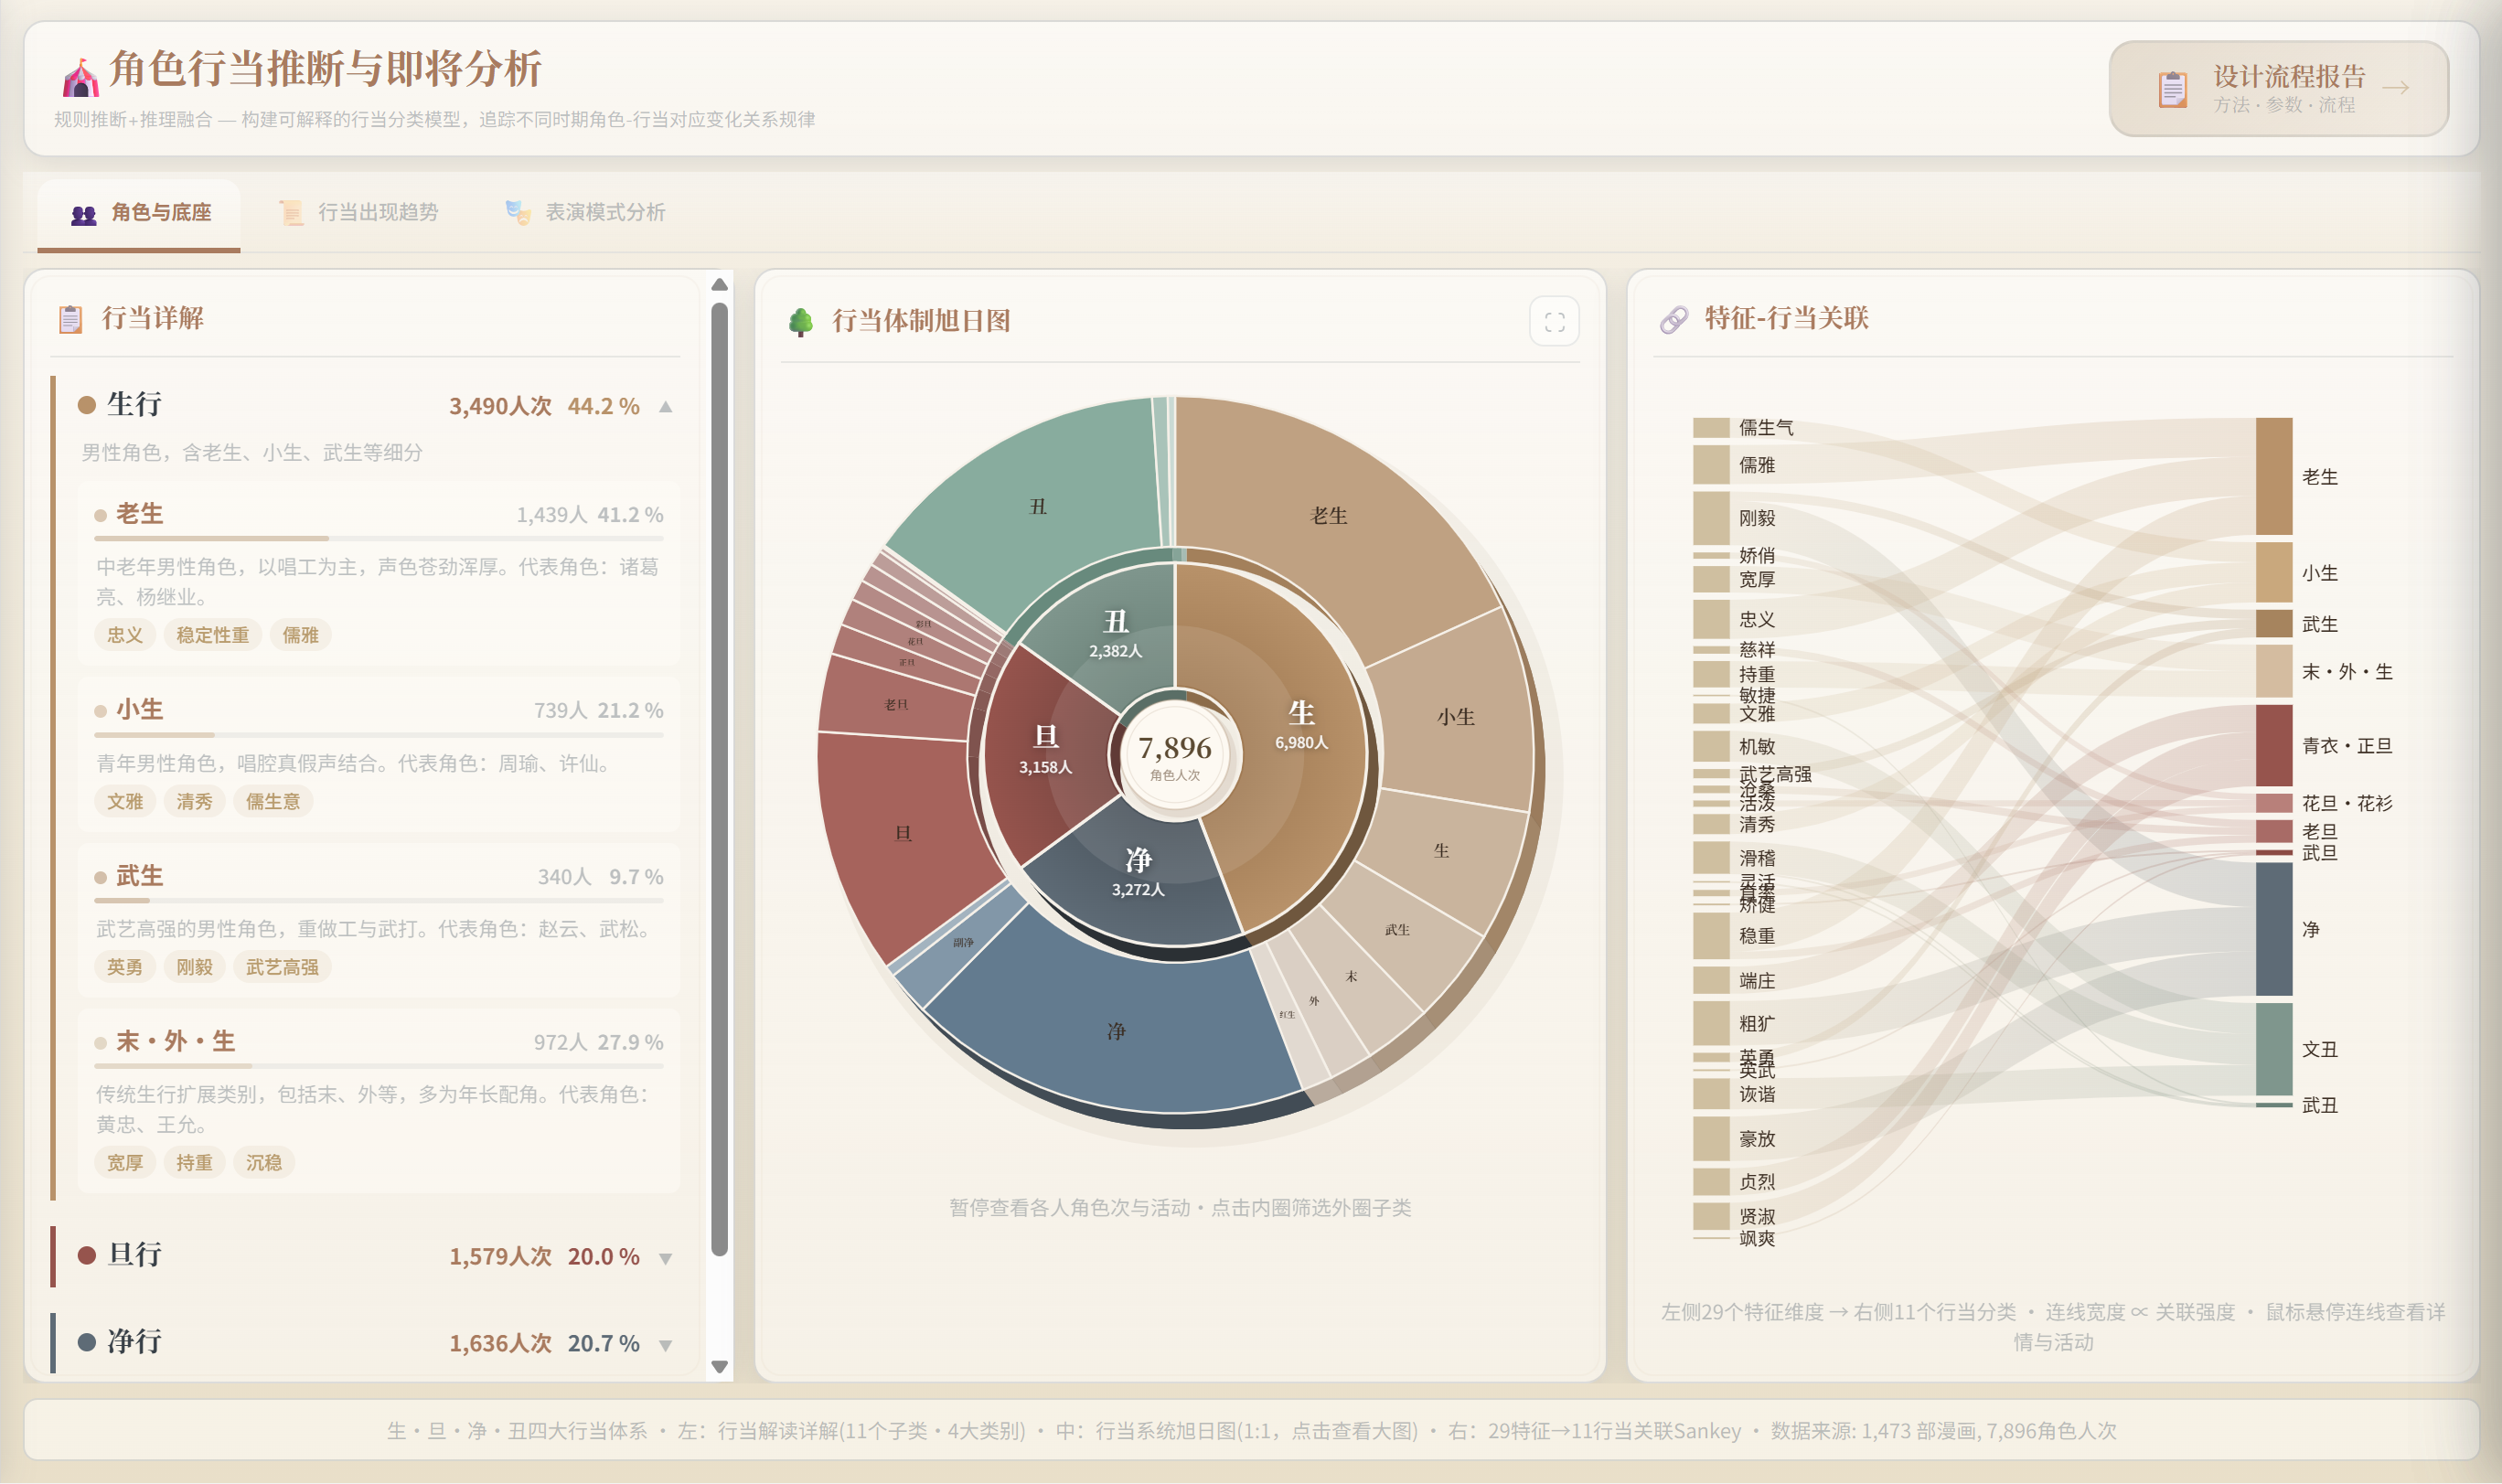
\includegraphics[width=\textwidth]{Image/Task1.png}
\end{minipage}%
\begin{minipage}[t]{0.50\textwidth}
  \centering
  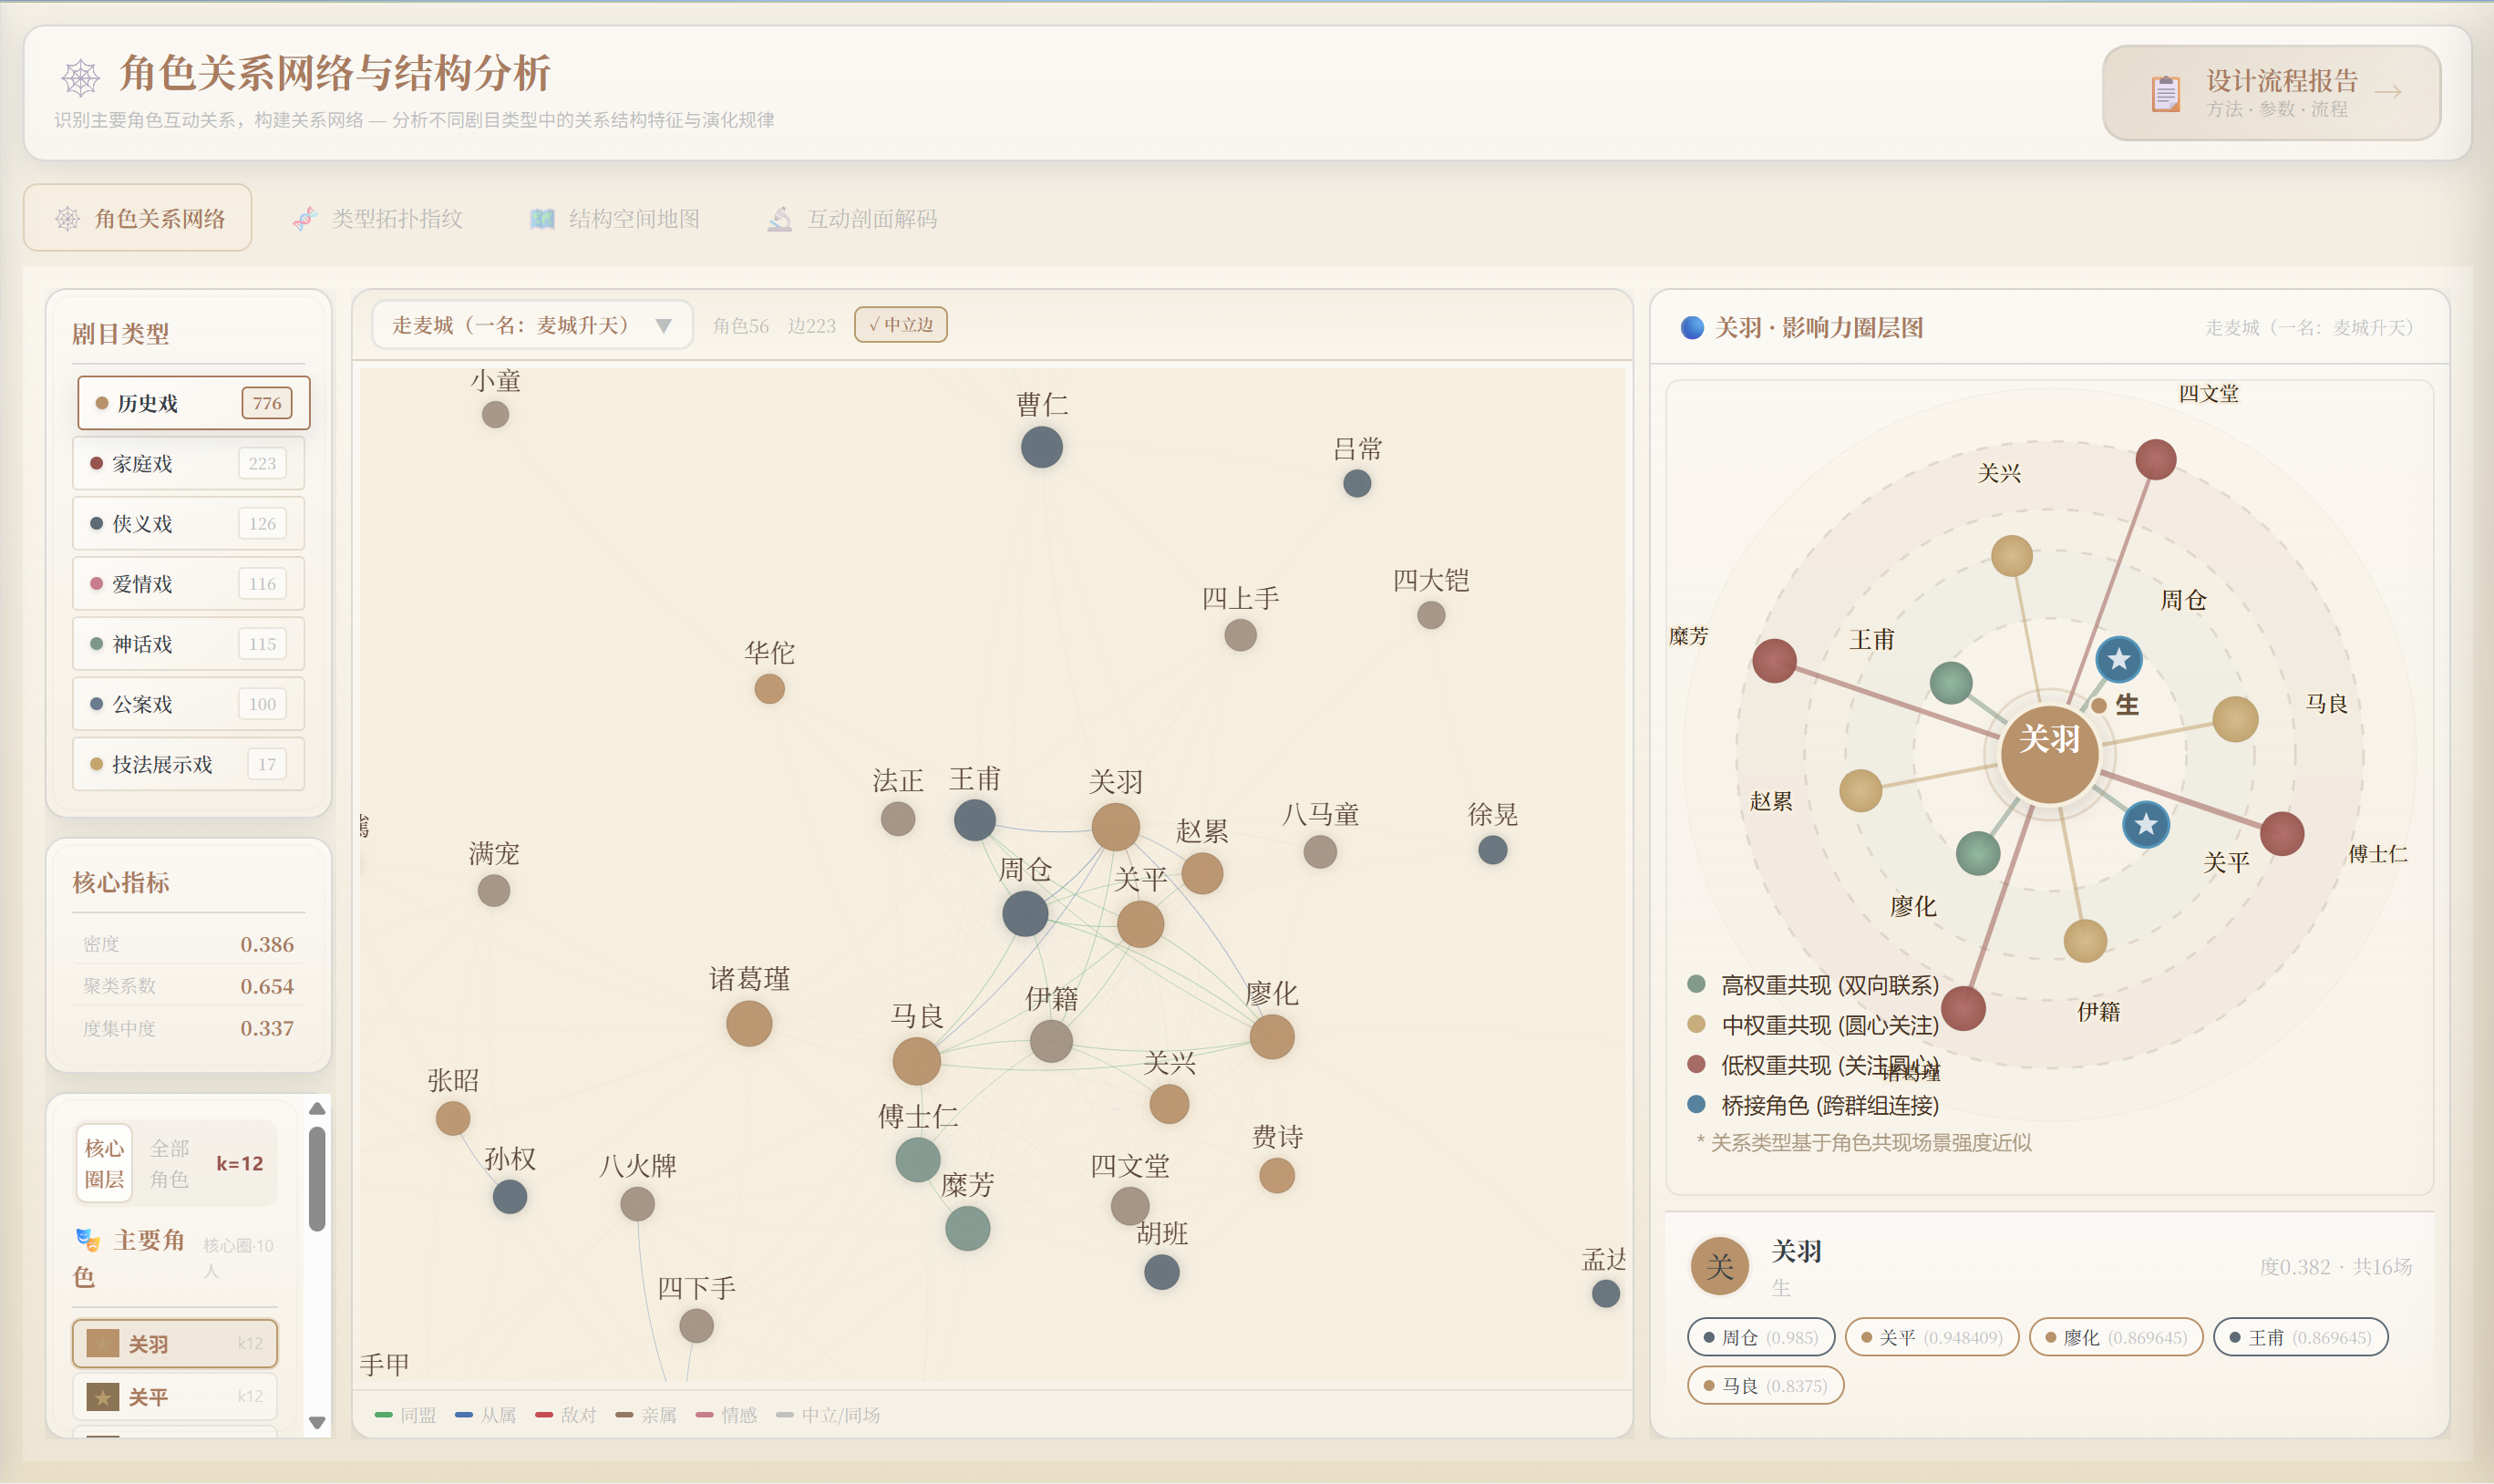
\includegraphics[width=\textwidth]{Image/Task2.png}
\end{minipage}

\vspace{-0.1em}

\begin{minipage}[t]{0.50\textwidth}
  \centering
  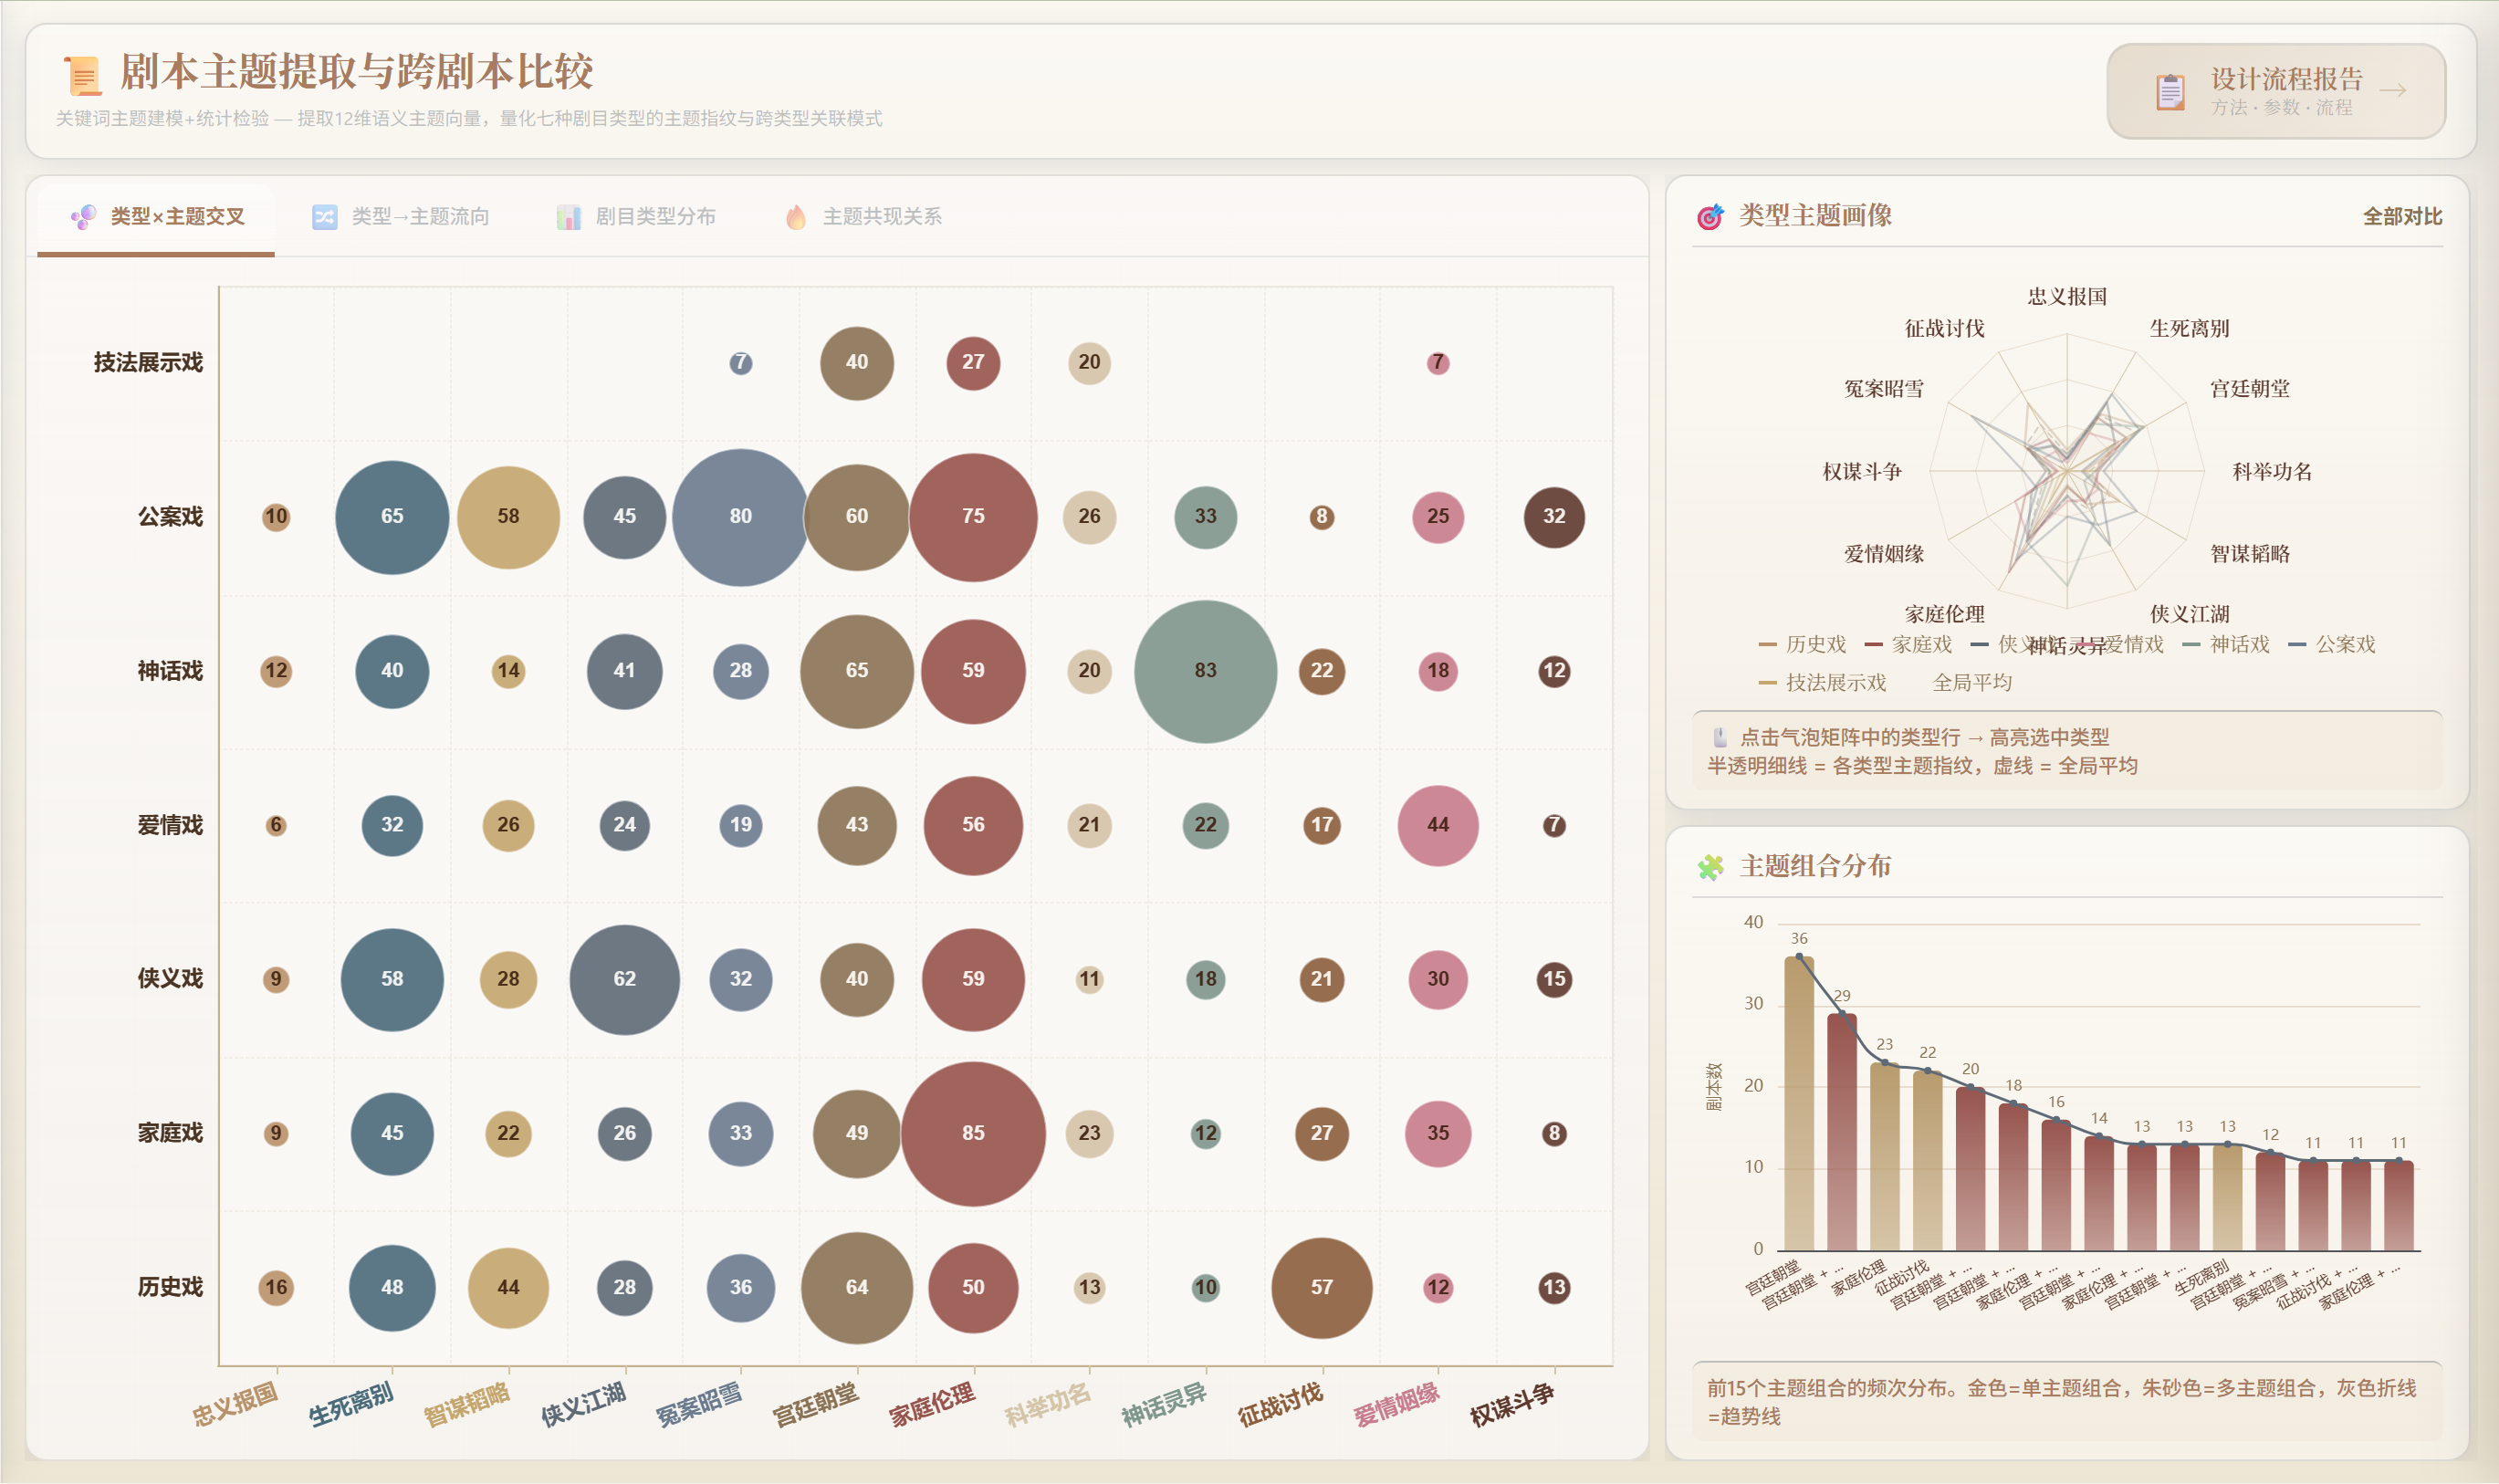
\includegraphics[width=\textwidth]{Image/Task3.png}
\end{minipage}%
\begin{minipage}[t]{0.50\textwidth}
  \centering
  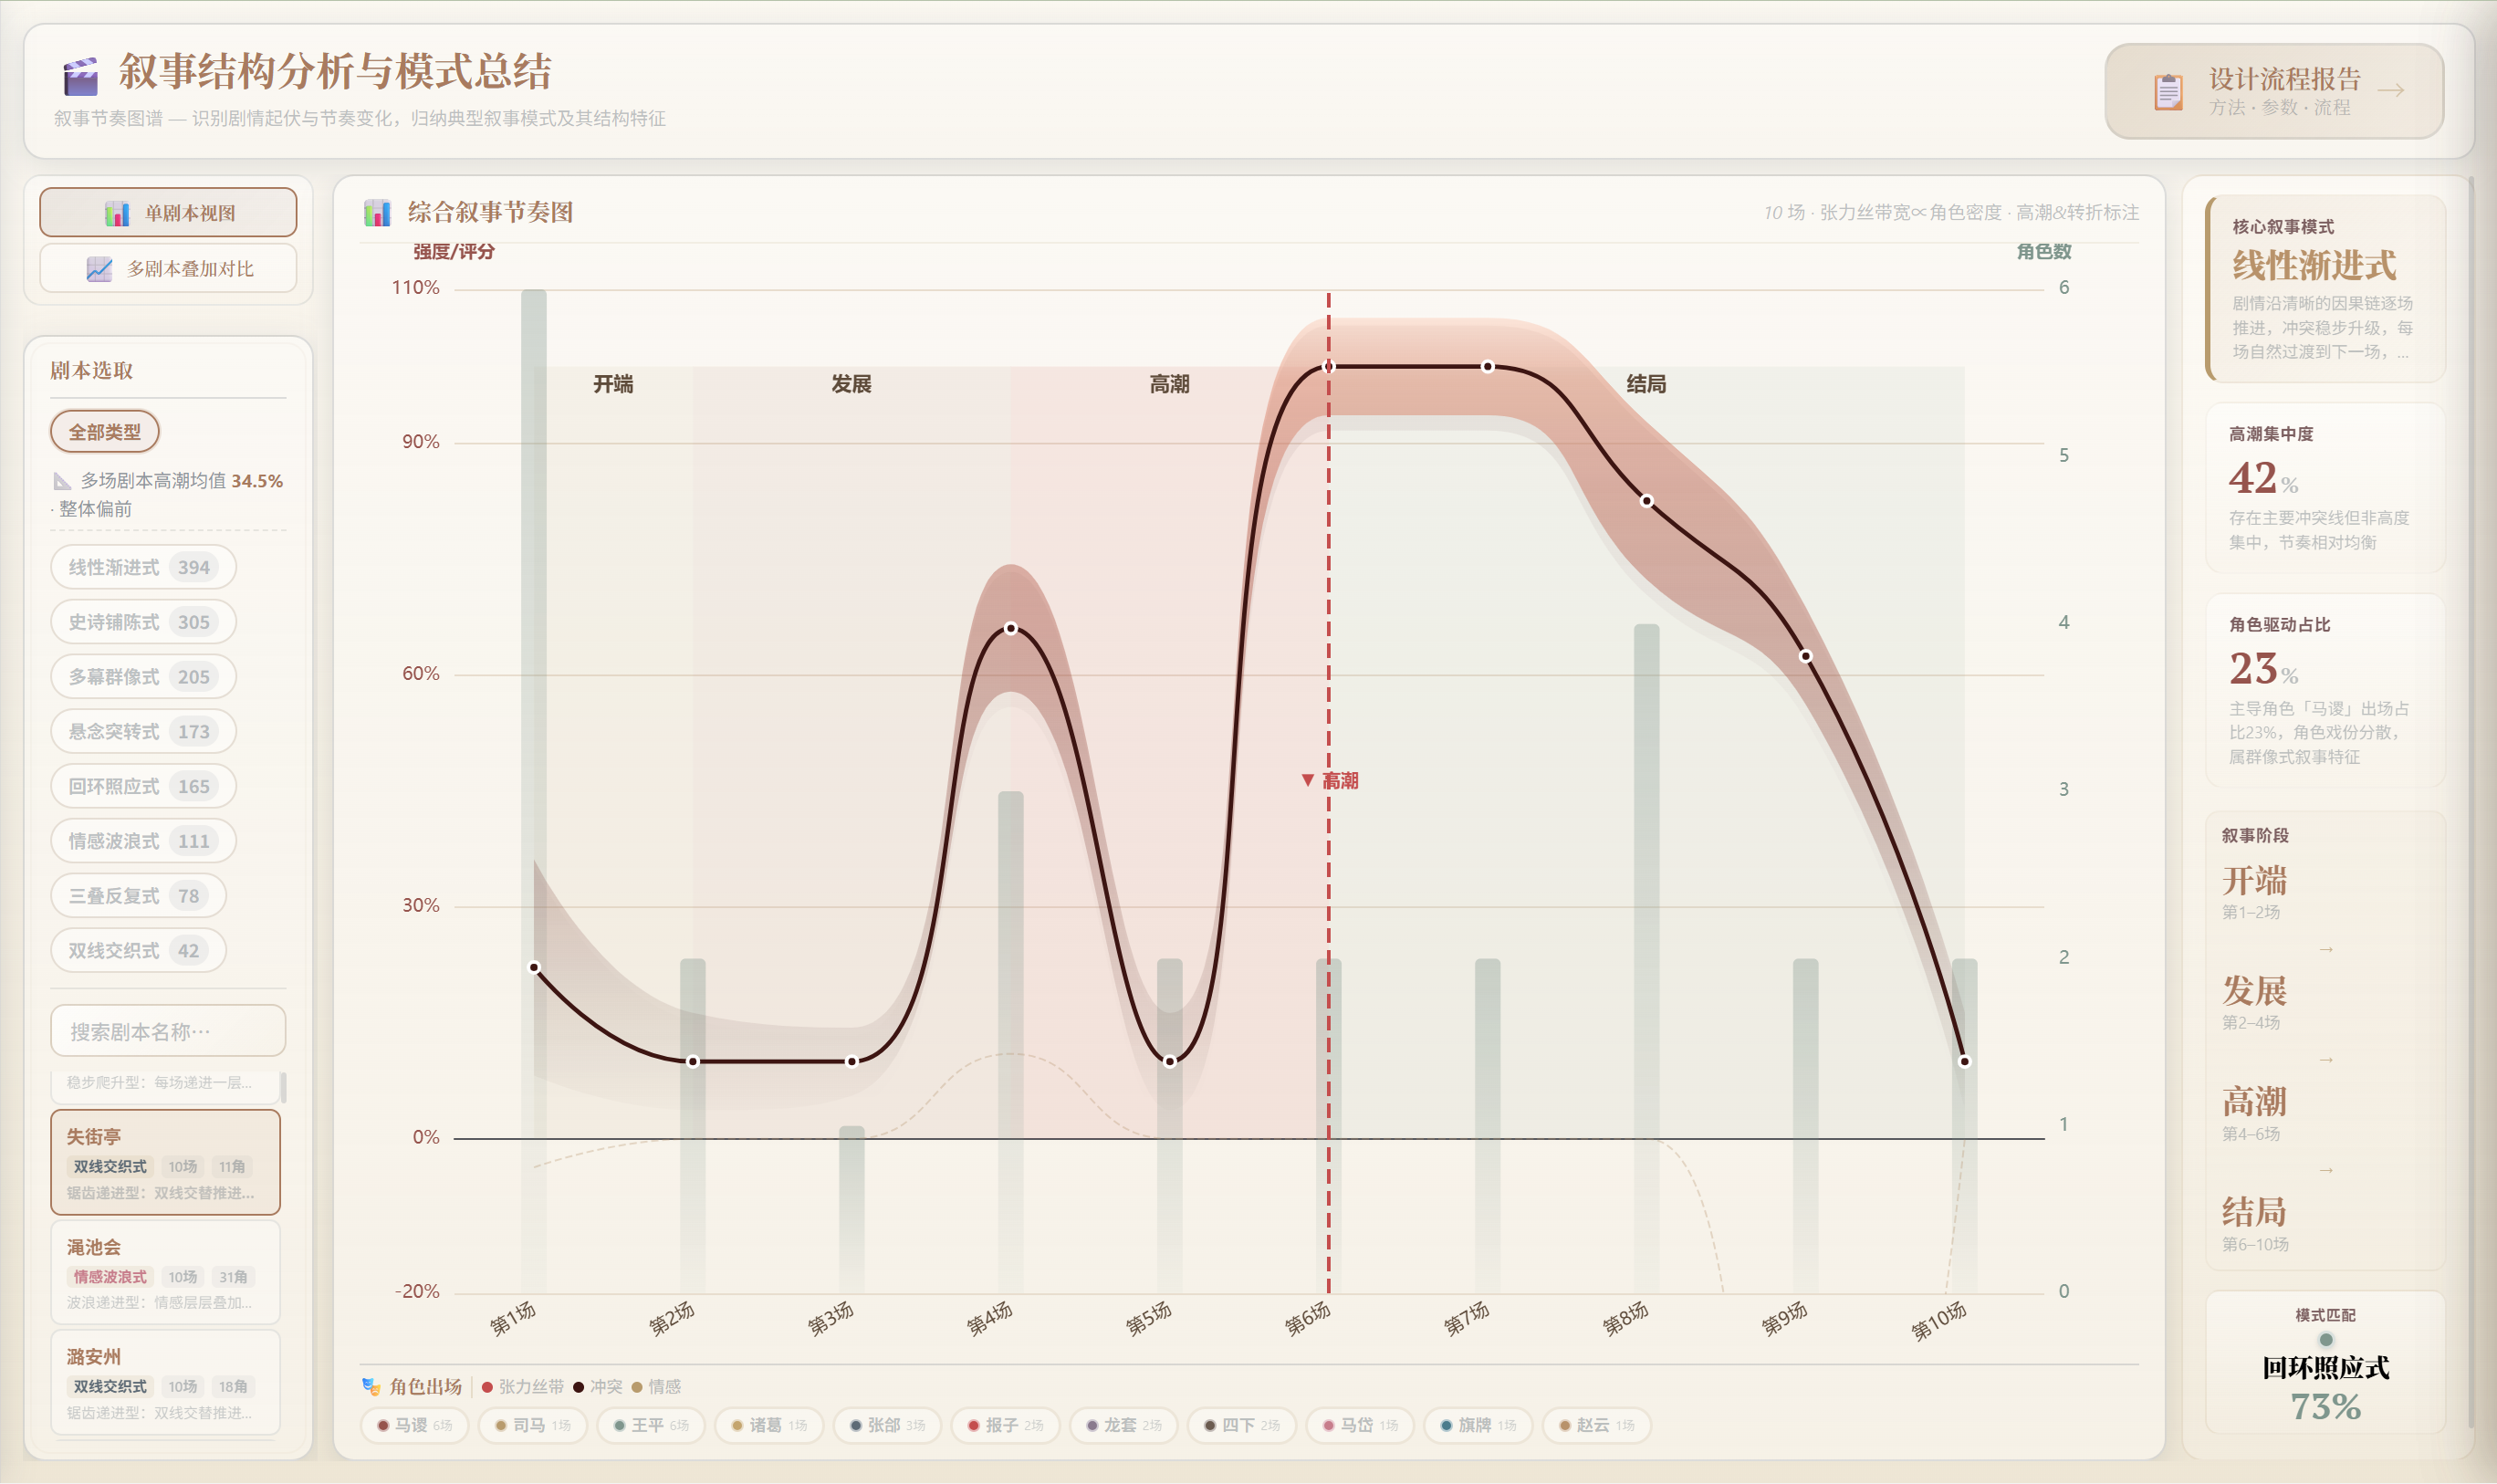
\includegraphics[width=\textwidth]{Image/Task4.png}
\end{minipage}
\caption{图0.3 任务一至任务四核心页面。}
\end{figure}

% {\fontsize{12bp}{20bp}\kaishu
% 任务一至任务四分别对应行当推断、角色关系、主题比较与叙事节奏四个分析入口。
% }

{\fontsize{12bp}{20bp}\kaishu
余下四个页面分别从四个维度展开分析（图0.3）：
\begin{itemize}[leftmargin=2.2em,itemsep=2pt,topsep=2pt]
\item \textbf{C. “行当推断”视图（左上）}：用角色行当旭日图呈现生、旦、净、丑及其细分支的整体层级结构，借助特征—行当桑基图梳理典型对应模式，并结合时期趋势图观察分布变化；支持结合典型角色个案查看行当判别依据。
\item \textbf{D. “角色关系”视图（右上）}：以力导向网络为主视图，配合类型指纹图、结构空间散点图和单剧关系剖面，比较不同剧目类型中的角色关系结构差异；支持切换代表性剧本，进一步查看单剧网络形态与互动关系。
\item \textbf{E. “主题结构”视图（左下）}：从跨剧本比较出发，以类型×主题气泡矩阵呈现不同剧本的主题覆盖情况，结合主题流向图和主题共现图整理主题组合原型及其差异；支持从类型比较继续定位到单剧主题构成。
\item \textbf{F. “叙事节奏”视图（右下）}：以单剧节奏曲线刻画冲突、情感和角色密度三条曲线形成的叙事阶段，通过多剧叠加对比图和模式总结图区分典型叙事方式；支持在单剧分析与多剧比较之间切换观察。
\end{itemize}
}

\vspace{5pt}

{\fontsize{12bp}{20bp}\kaishu
演示视频和作品高清文件已分别整理上传至 \href{https://www.bilibili.com/video/BV1jSjk6oELW/}{哔哩哔哩} 与 \href{https://pan.baidu.com/s/1V7-w7FQtu19aqaoNZouKhw?pwd=szyh}{百度网盘}。
}

% ============================================================
% 问题一
% ============================================================

{\fontsize{14bp}{22bp}\heiti\bfseries 任务一作品说明文档：}

\vspace{10pt}

{\fontsize{13bp}{20bp}\heiti\bfseries
1、基于剧本中角色的性别、年龄、身份、性格描述及唱念做打等表演提示，推断未标注角色的行当归属（如生、旦、净、丑及其细分支），并分析角色特征与行当分类之间的典型对应模式。进一步结合剧本创作年代或历史时期背景，利用数据分析和可视化等手段，探究不同时期角色-行当对应关系的变化规律。
}

\vspace{6pt}

{\fontsize{13bp}{18bp}\heiti\bfseries 1.1 角色特征整理与总体判断}

\vspace{4pt}

{\fontsize{12bp}{20bp}\kaishu
我们先把 1{,}473 部剧本中的角色性别、年龄、身份、性格描述以及唱念做打等表演提示整理成可比较的文本标签，并进一步归纳为 29 个核心维度、11 条推断规则，再据此统计角色特征与行当类别之间的对应关系；随后结合典型角色个案，对生、旦、净、丑及其细分支的判别依据做交叉验证，并按编纂出版来源观察不同时期的角色—行当分布差异。
}

{\fontsize{12bp}{20bp}\kaishu
放到整体样本中比较后，我们看到，在 7{,}896 个角色人次与 3{,}581 个独立角色的范围内，角色特征与行当之间存在极强关联（\ensuremath{\chi^2}=204{,}444，\textit{df}=280，p<0.001；关联强度 Cramér's V=0.949）；同时，658 个角色（18.4\%）在不同剧本中出现跨行当现象。这说明未标注角色的行当大多可以通过文本特征作出较稳定的推断，但这种对应关系并非完全刚性，在不同来源和时期中仍会出现局部调整。
}

\vspace{6pt}

{\fontsize{13bp}{18bp}\heiti\bfseries 1.2 四大行当的典型对应方式}

\vspace{4pt}

{\fontsize{12bp}{20bp}\kaishu
\begin{itemize}[leftmargin=2.2em,itemsep=2pt,topsep=2pt]
\item \textbf{生行}：代表子类包括老生、小生、武生、末外生、红生。其典型特征是男性、壮年或老年、身份偏文臣将帅，常对应忠义、稳重等气质，因此“宽厚 $\rightarrow$ 末外生”、“武艺高强 $\rightarrow$ 武生”一类映射最稳定。
\item \textbf{旦行}：代表子类包括青衣正旦、花旦花衫、老旦、武旦。其内部区分最明显，通常由年龄、性格与舞台气质共同决定，如“活泼 $\rightarrow$ 花旦花衫”、“端庄贞烈 $\rightarrow$ 青衣正旦”。
\item \textbf{净行}：代表子类包括净、副净、武净。其角色多表现为刚烈、豪放、威严和高对抗性，因此“豪放刚烈 $\rightarrow$ 净”更常见，外显特征也最鲜明。
\item \textbf{丑行}：代表子类包括文丑、武丑、丑旦。其角色通常机敏、滑稽，或承担串联场面的功能，因此“滑稽机敏 $\rightarrow$ 文丑”、“敏捷灵活 $\rightarrow$ 武丑”具有较稳定的对应关系。
\end{itemize}
}

{\fontsize{12bp}{20bp}\kaishu
从整体占比看，四大行当的分布约为：生行 44.2\%、旦行 20.0\%、净行 20.7\%、丑行 15.1\%。这说明京剧剧本总体呈现“\textbf{生行为主、旦净并列、丑行辅助}”的结构格局（图1.1）。
}

% ================= 图1.1：总体模式拼图 =================
% 文件存放位置：Image/q1-2-overview-collage.png
% 图片内容：左图必须使用行当层级旭日图，展示四大行当及细分支的层级结构与占比；右图使用特征-行当 Sankey 图，展示性别/身份/性格/表演提示到行当的流向
% 使用方法：图片准备好后，取消下方 figure 注释即可
%
\begin{figure}[H]
\centering
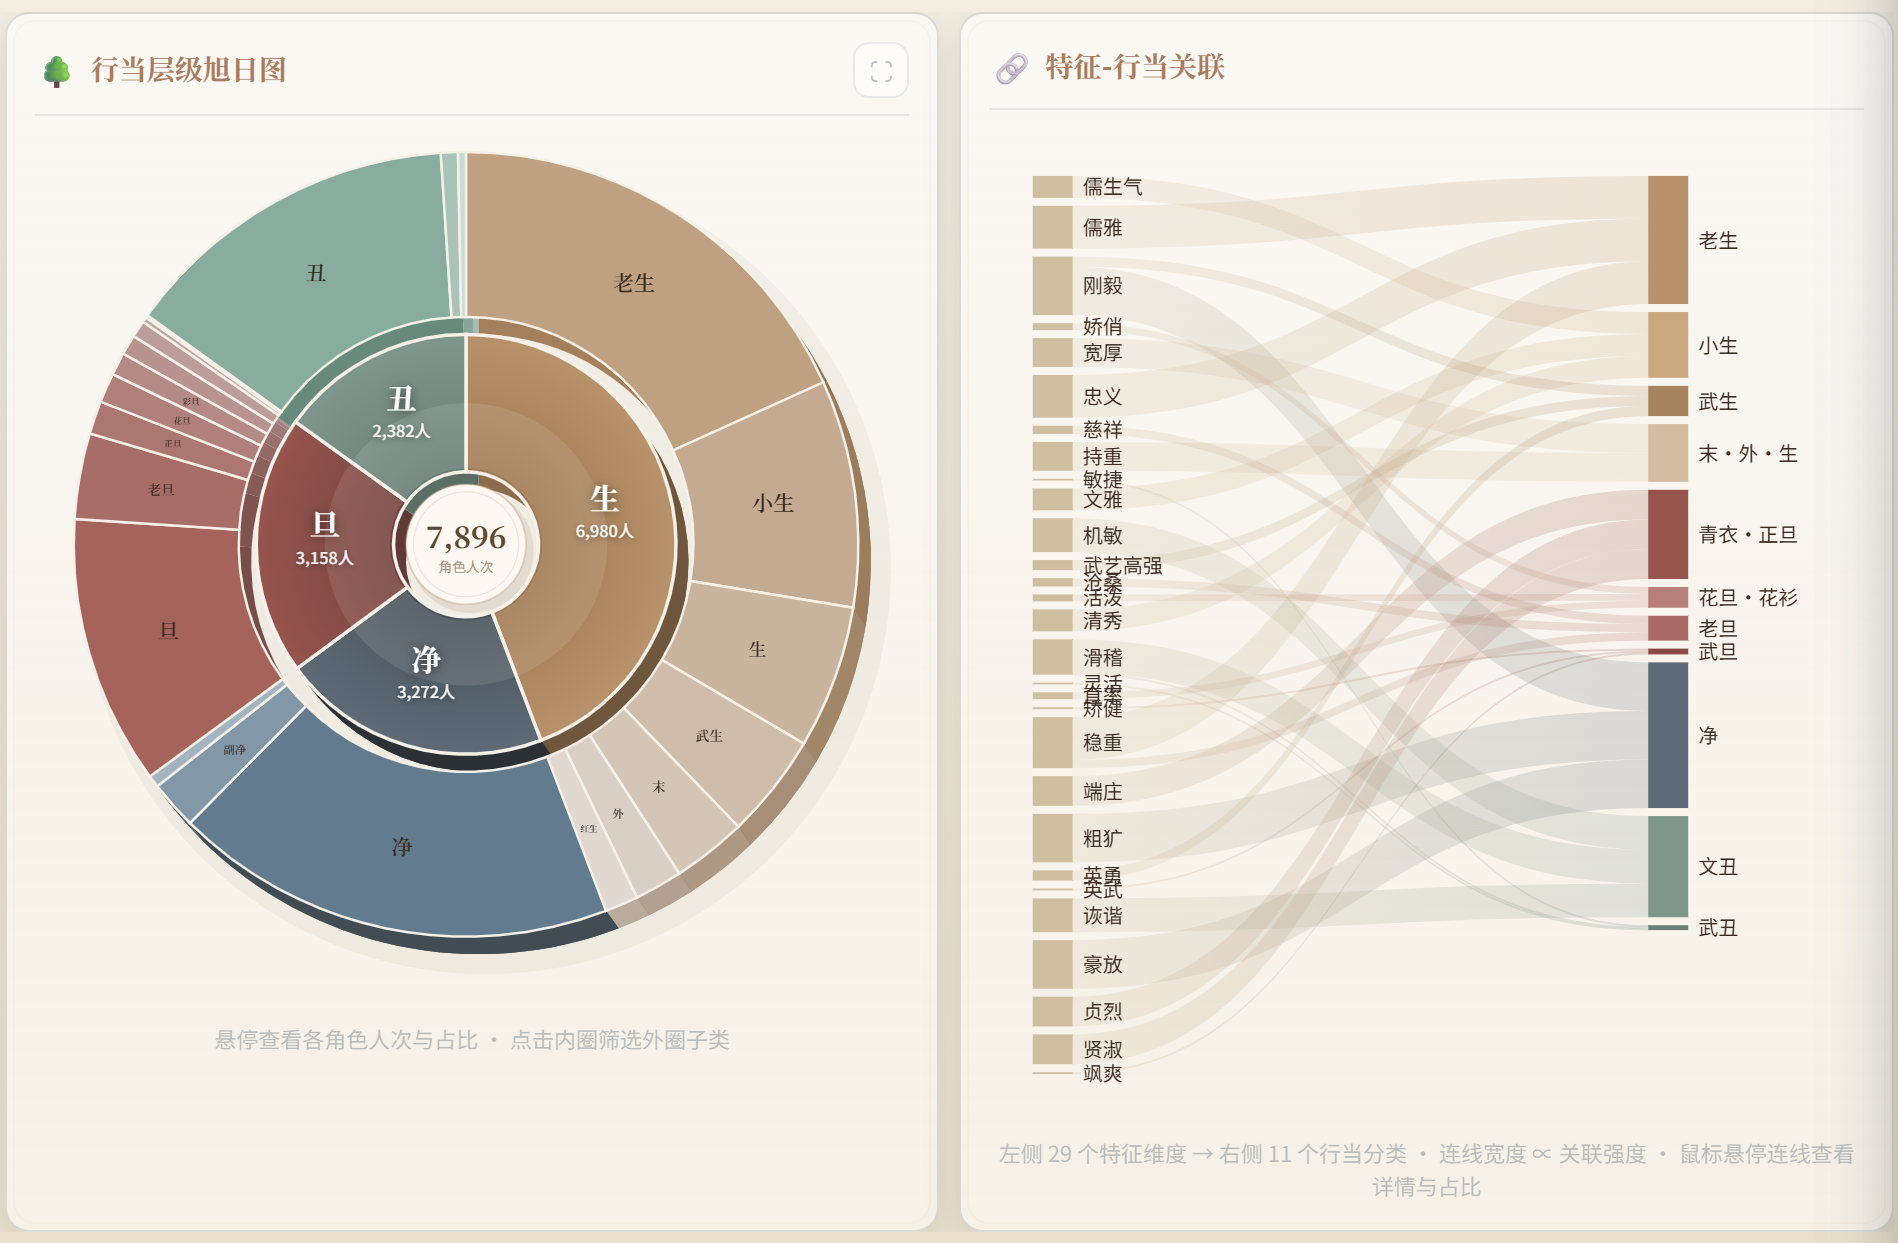
\includegraphics[width=0.95\textwidth]{Image/q1-2-overview-collage.png}
\caption{图1.1 角色—行当整体结构与特征对应关系}
\end{figure}

{\fontsize{12bp}{20bp}\kaishu
以关羽为例，并与诸葛亮、曹操作对比可以看到，关羽在现有剧本标注中多数以红生出现；放到表演模式分析中看，他同时具有较高念白占比和一定武打成分，因此更适合放在红生这一兼具文武气质的位置上理解。这说明行当判断并非只看单一特征，而是要结合身份、性格与表演方式综合判断（图1.2）。
}

% ================= 图1.2：典型角色对比图 =================
% 文件存放位置：Image/q1-2-role-case-guanyu.png
% 图片内容：典型角色雷达图或角色卡片，展示关羽，并与诸葛亮、曹操作对比
% 使用方法：图片准备好后，取消下方 figure 注释即可
%
\begin{figure}[H]
\centering
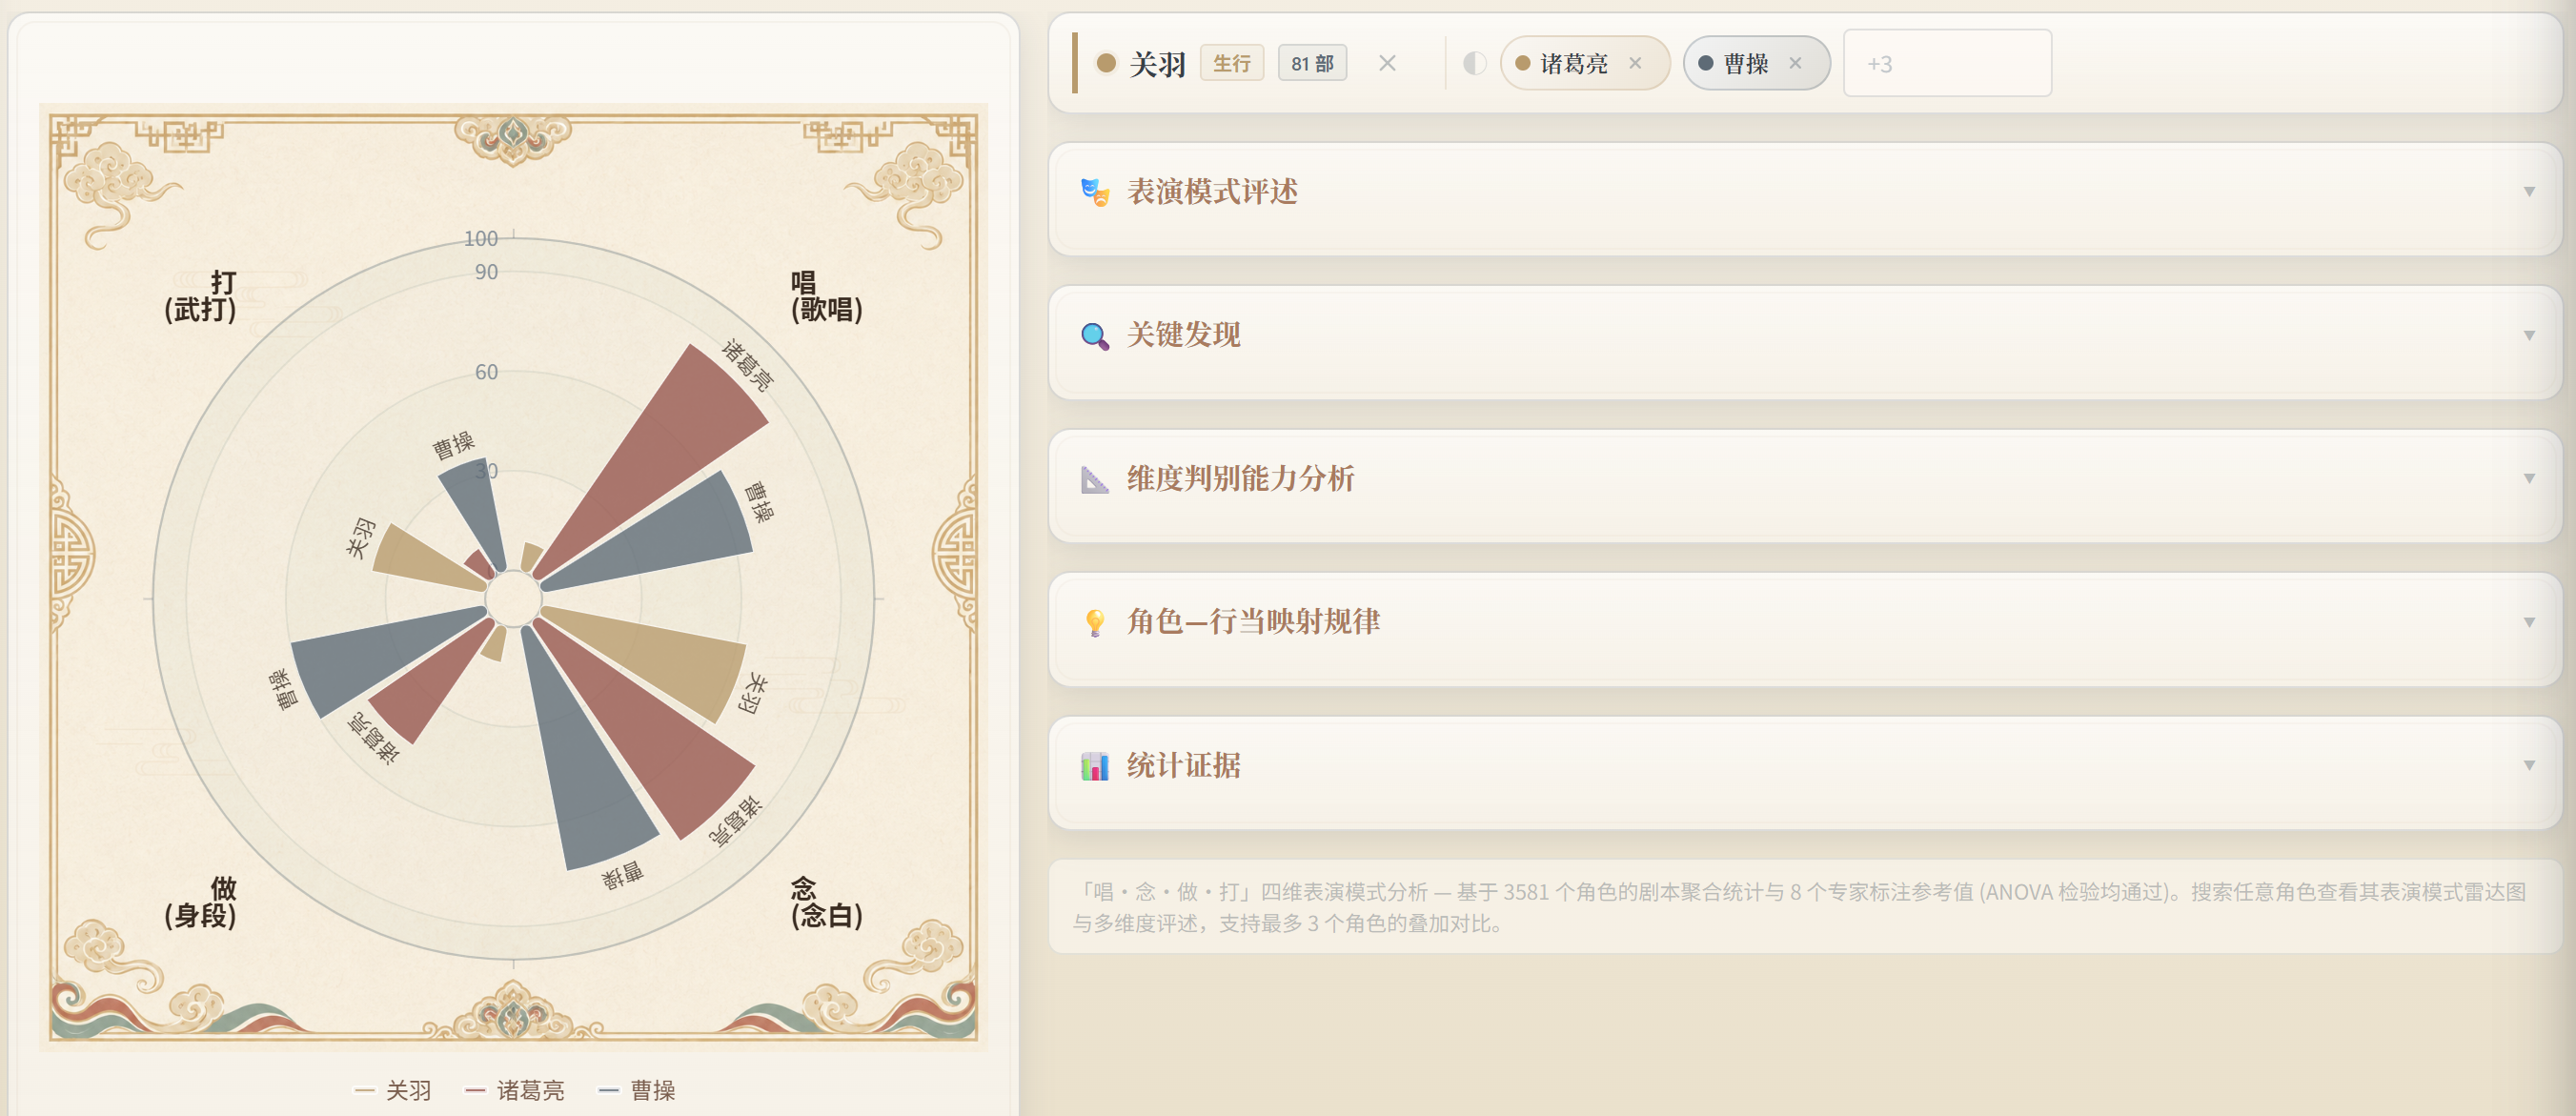
\includegraphics[width=0.95\textwidth]{Image/q1-2-role-case-guanyu.png}
\caption{图1.2 典型角色对比：关羽、诸葛亮与曹操的行当判别依据}
\end{figure}

% \vspace{6pt}

{\fontsize{13bp}{18bp}\heiti\bfseries 1.3 六类来源时期中的行当变化}

% \vspace{4pt}

{\fontsize{12bp}{20bp}\kaishu
由于现有剧本数据的时间信息主要体现为\textbf{编纂出版来源所对应的整理出版时期}，因此我们据此观察六类时期下角色—行当关系的变化。卡方检验表明，不同时期的分布差异显著（\ensuremath{\chi^2}=82.3，\textit{df}=15，p<0.001），但关联强度较小（Cramér's V=0.059），说明变化存在，但总体仍以稳定延续为主。
}

\vspace{4pt}
{\fontsize{12bp}{20bp}\kaishu
从六类来源时期的分布来看（图1.3），大致可以看到三个阶段：
\begin{enumerate}[leftmargin=2.2em,itemsep=2pt,topsep=2pt]
\item \textbf{稳定延续阶段}：主要对应民国汇编本和新中国整理本，此时生行始终保持高位，净行也维持较强存在，四大行当的主次格局最为清晰。
\item \textbf{局部偏移阶段}：主要见于昆曲剧本选和名家演出本。前者旦行占比有所抬升，净、丑则相对收缩；后者四类占比更接近均衡，说明不同流派与整理方式会改变四大行当的组合重心。
\item \textbf{结构趋衡阶段}：主要出现在现代剧作家本和录音藏本及其他来源，生旦净丑之间的差距进一步缩小，整体呈现由单一主导走向相对均衡的倾向，但这部分样本量较小，因此只适合作为谨慎观察。
\end{enumerate}
}

% ================= 图1.3：时期变化图 =================
% 文件存放位置：Image/q1-3-period-trend-collage.png
% 图片内容：左图为四大行当随来源时期变化的折线图或堆叠面积图；右图为相对增长率热力图或时期差异矩阵
% 使用方法：图片准备好后，取消下方 figure 注释即可
%
\begin{figure}[H]
\centering
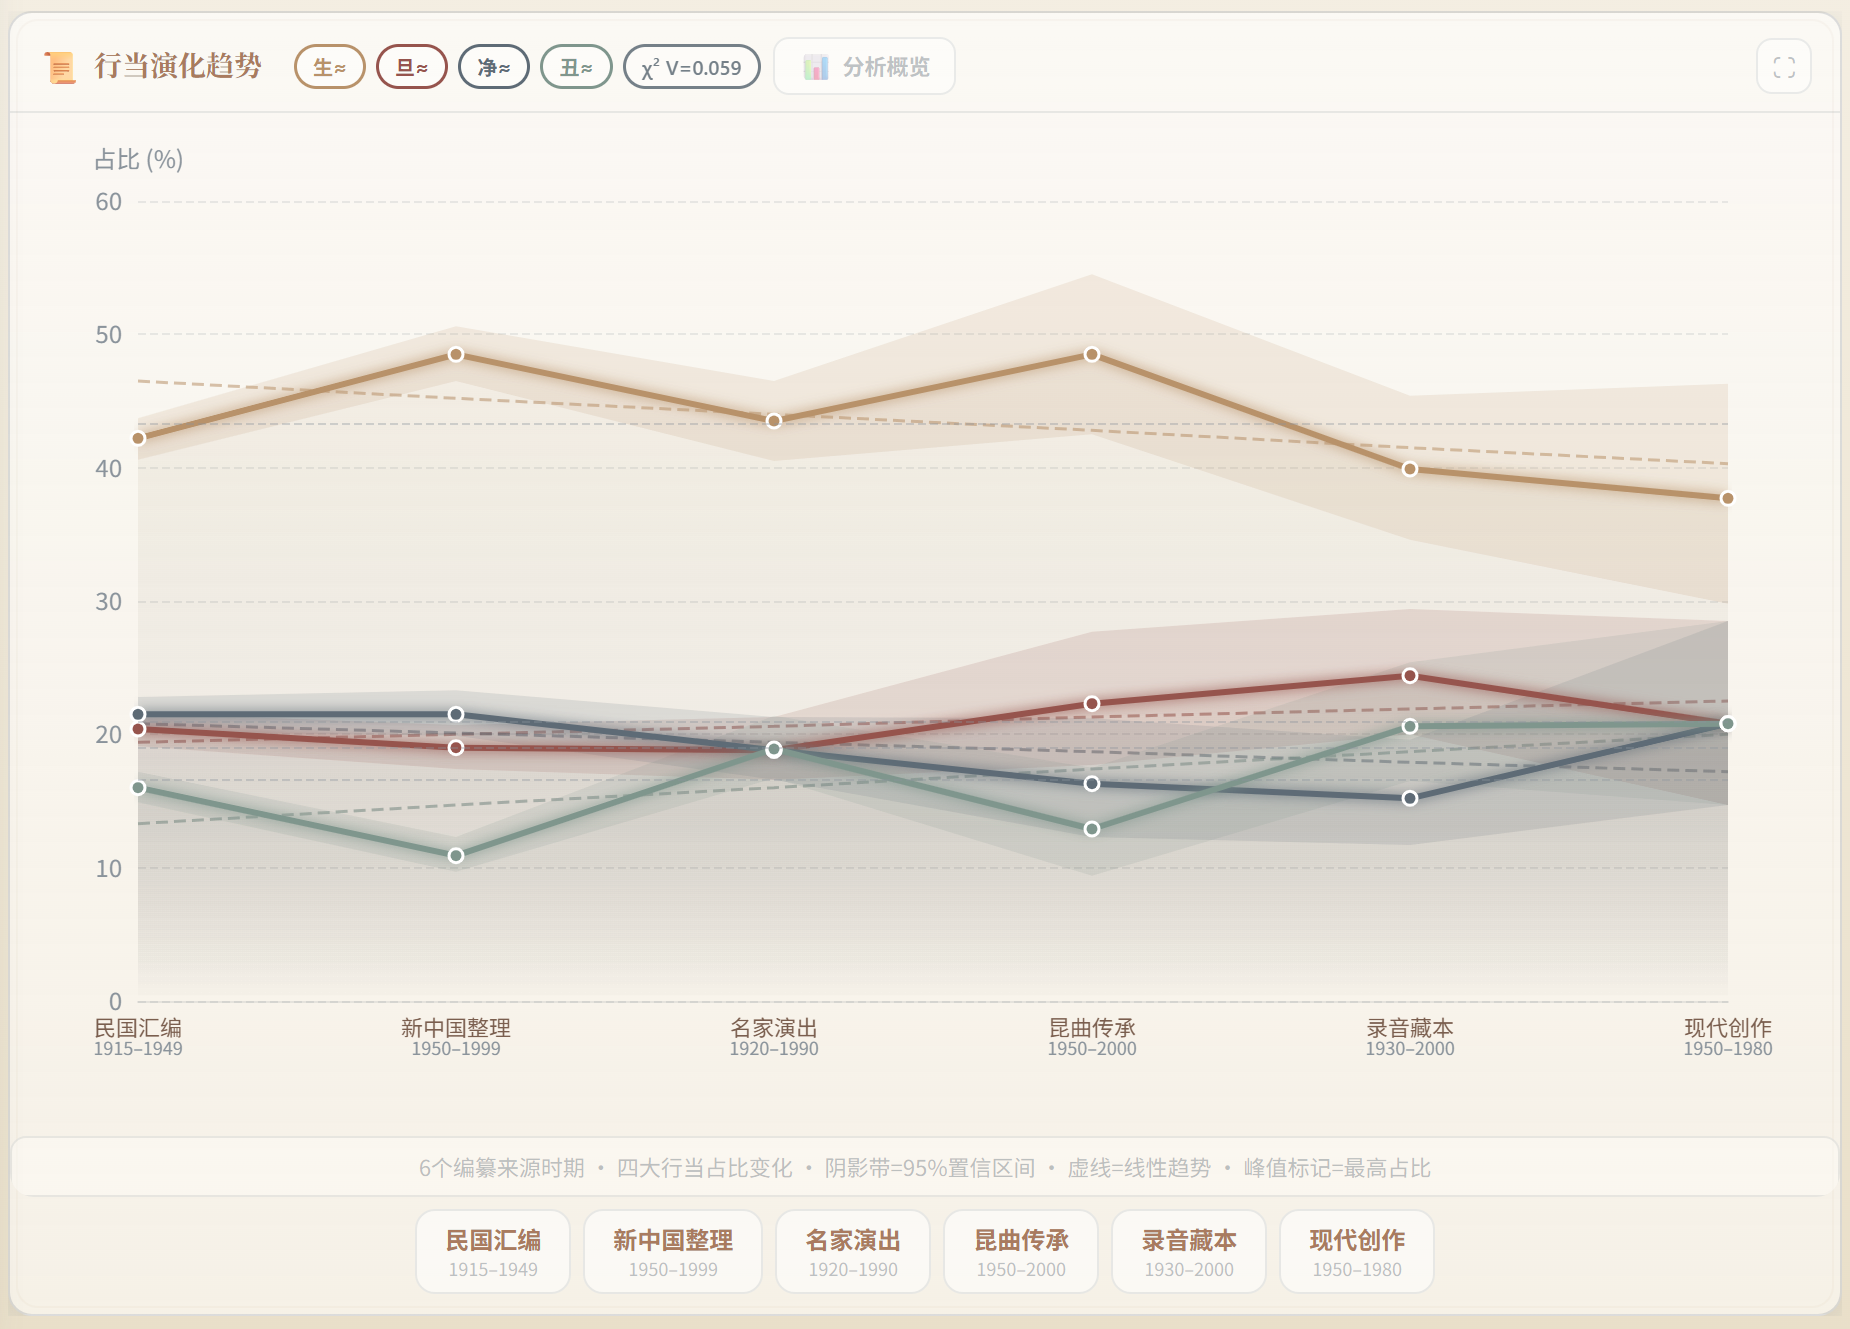
\includegraphics[width=0.95\textwidth]{Image/q1-3-period-trend-collage.png}
\caption{图1.3 不同时期角色—行当关系的变化趋势}
\end{figure}

{\fontsize{13bp}{18bp}\heiti\bfseries 1.4 综合判断}

% \vspace{4pt}

{\fontsize{12bp}{20bp}\kaishu
综合来看，我们认为未标注角色的行当大多可以通过文本特征进行较稳定的推断；从总体格局看，角色—行当对应关系主要表现为四类典型方式，不同时期下的分布虽然会受来源与流派影响出现局部调整，但生旦净丑这一基本框架并未发生根本变化。
}

% \vspace{10pt}

% ============================================================
% 问题二
% ============================================================

{\fontsize{13bp}{20bp}\heiti\bfseries
2、请识别剧本中主要角色之间的互动关系，构建角色关系网络，并分析不同剧目（历史戏、家庭戏、公案戏等）中的角色关系网络结构特征。
}

\vspace{6pt}

{\fontsize{13bp}{18bp}\heiti\bfseries 2.1 关系提取方式与整体差异}

\vspace{4pt}

{\fontsize{12bp}{20bp}\kaishu
我们先按场景切分 1{,}473 部剧本，提取同场出现的角色，再结合文本语义把边划分为同盟、从属、敌对、亲属、情感五类关系，最终为每部剧本构建一张角色关系网络；在此基础上，再从网络密度（连接紧密程度）、中心性偏离度（是否由单一角色主导）、聚类系数（小团体闭合程度）等 8 项指标出发，对七类剧目进行比较。
}

{\fontsize{12bp}{20bp}\kaishu
从整体检验结果看，我们发现单因素方差分析（ANOVA）与 Kruskal-Wallis 检验都指出，这 8 项指标在不同剧目之间均存在显著差异（p<0.001）。这说明剧目类型不仅影响人物和情节题材，也会稳定影响角色关系的组织方式。
}

\vspace{6pt}

{\fontsize{13bp}{18bp}\heiti\bfseries 2.2 七类剧目的关系网络画像}

\vspace{4pt}

{\fontsize{10.5bp}{15bp}\selectfont
\renewcommand{\arraystretch}{1.25}
\begin{center}
\begin{tabular}{C{0.16\textwidth} L{0.22\textwidth} L{0.24\textwidth} L{0.22\textwidth}}
\toprule
剧目类型 & 主要结构 & 统计特征 & 说明 \tabularnewline
\midrule
历史戏 & 群像分散、阵营对立 & 密度最低 0.386 & 人物多、冲突线多，更接近“战场式”铺陈 \tabularnewline
家庭戏 & 亲缘团块、多核心均衡 & 亲属关系占比最高 41.1\%，密度 0.558 & 互动围绕家庭内部展开，更接近“家族合影” \tabularnewline
爱情戏 & 双核收束、情感驱动 & 密度 0.615，中心性偏离度最低 0.226，情感关系占比最高 12.2\% & 关系主要围绕男女主角收束，而非由单一角色垄断 \tabularnewline
侠义戏 & 英雄辐射、跨圈连接 & 中心性偏离度最高 0.344 & 主角常连接江湖、官府与同盟圈层 \tabularnewline
公案戏 & 审案核心、分层扩散 & 从属关系占比最高 40.2\%，密度 0.456 & 官员、衙役与当事人形成较明显的层级结构 \tabularnewline
神话戏 & 高闭合小团体并置 & 聚类系数最高 0.754 & 仙佛、妖魔与凡间人物常以小团体方式交织出现 \tabularnewline
技法展示戏 & 极简高密、角色最少 & 密度最高 0.775 & 角色少、同台频繁，更强调表演展示 \tabularnewline
\bottomrule
\end{tabular}
\end{center}
}

% ================= 图2.1：类型指纹拼图 =================
% 文件存放位置：Image/q2-2-fingerprint-collage.png
% 图片内容：左图使用“结构标签流向·冲积图”，展示七类剧目到结构标签的分布；右图使用“指标偏差热力矩阵”，展示各类型在网络密度、中心性偏离度、聚类系数等指标上的标准化差异
% 使用方法：图片准备好后，取消下方 figure 注释即可
%
\begin{figure}[H]
\centering
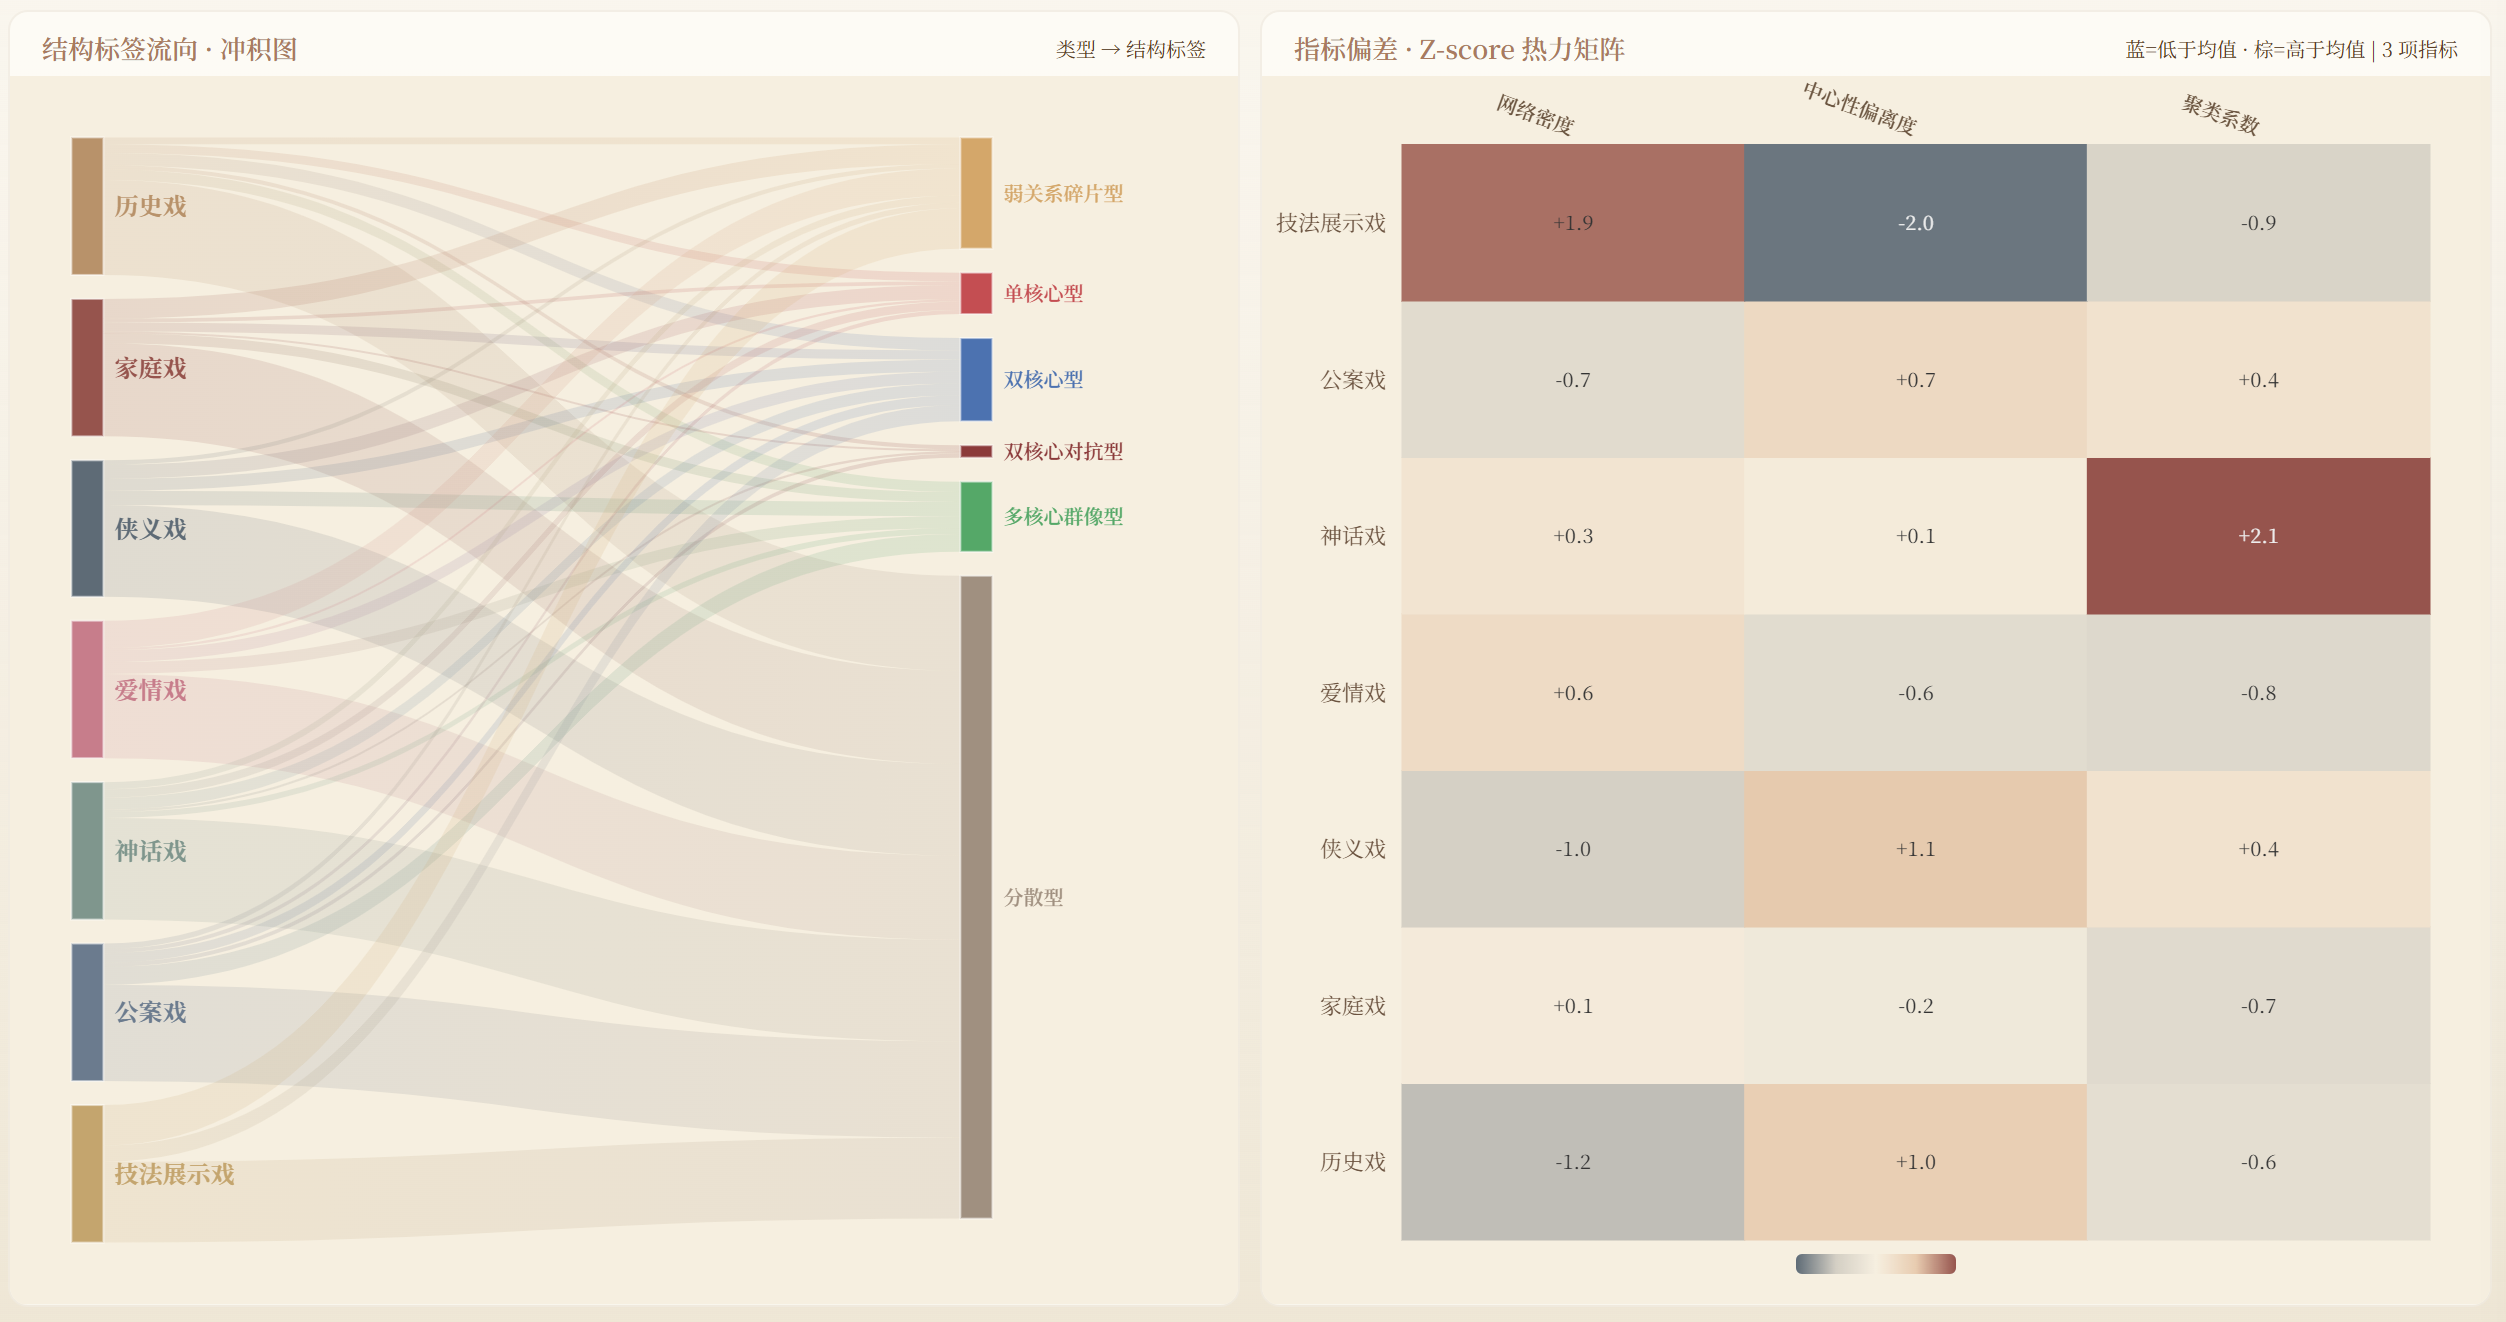
\includegraphics[width=1.0\textwidth]{Image/q2-2-fingerprint-collage.png}
\caption{图2.1 不同剧目类型的关系结构指纹}
\end{figure}

\vspace{6pt}

{\fontsize{13bp}{18bp}\heiti\bfseries 2.3 结构空间中的类型分布与单剧验证}

\vspace{4pt}
{\fontsize{12bp}{20bp}\kaishu
把 1{,}473 部剧本放到同一结构空间后，上述差异会更直观。增强 PCA 散点图中，横轴更接近“去中心化—高度集中”，纵轴更接近“碎片化—高度连通”。据此可以看到，历史戏与公案戏整体更靠中下部，侠义戏更偏向右侧的高集中区域，家庭戏、爱情戏和神话戏则更靠上方的高连通区域；技法展示戏因为角色极少，进一步落在高连通的极端位置。也就是说，不同剧目并不是杂乱混在一起，而是会围绕各自的结构重心形成相对稳定的“结构指纹”（图2.2）。
}

% ================= 图2.2：结构空间地图 =================
% 文件存放位置：Image/q2-3-space-map.png
% 图片内容：使用“结构空间地图”页面的 PCA 散点图，保留七类剧目点云、类型质心与图例
% 使用方法：图片准备好后，取消下方 figure 注释即可
%
\begin{figure}[H]
\centering
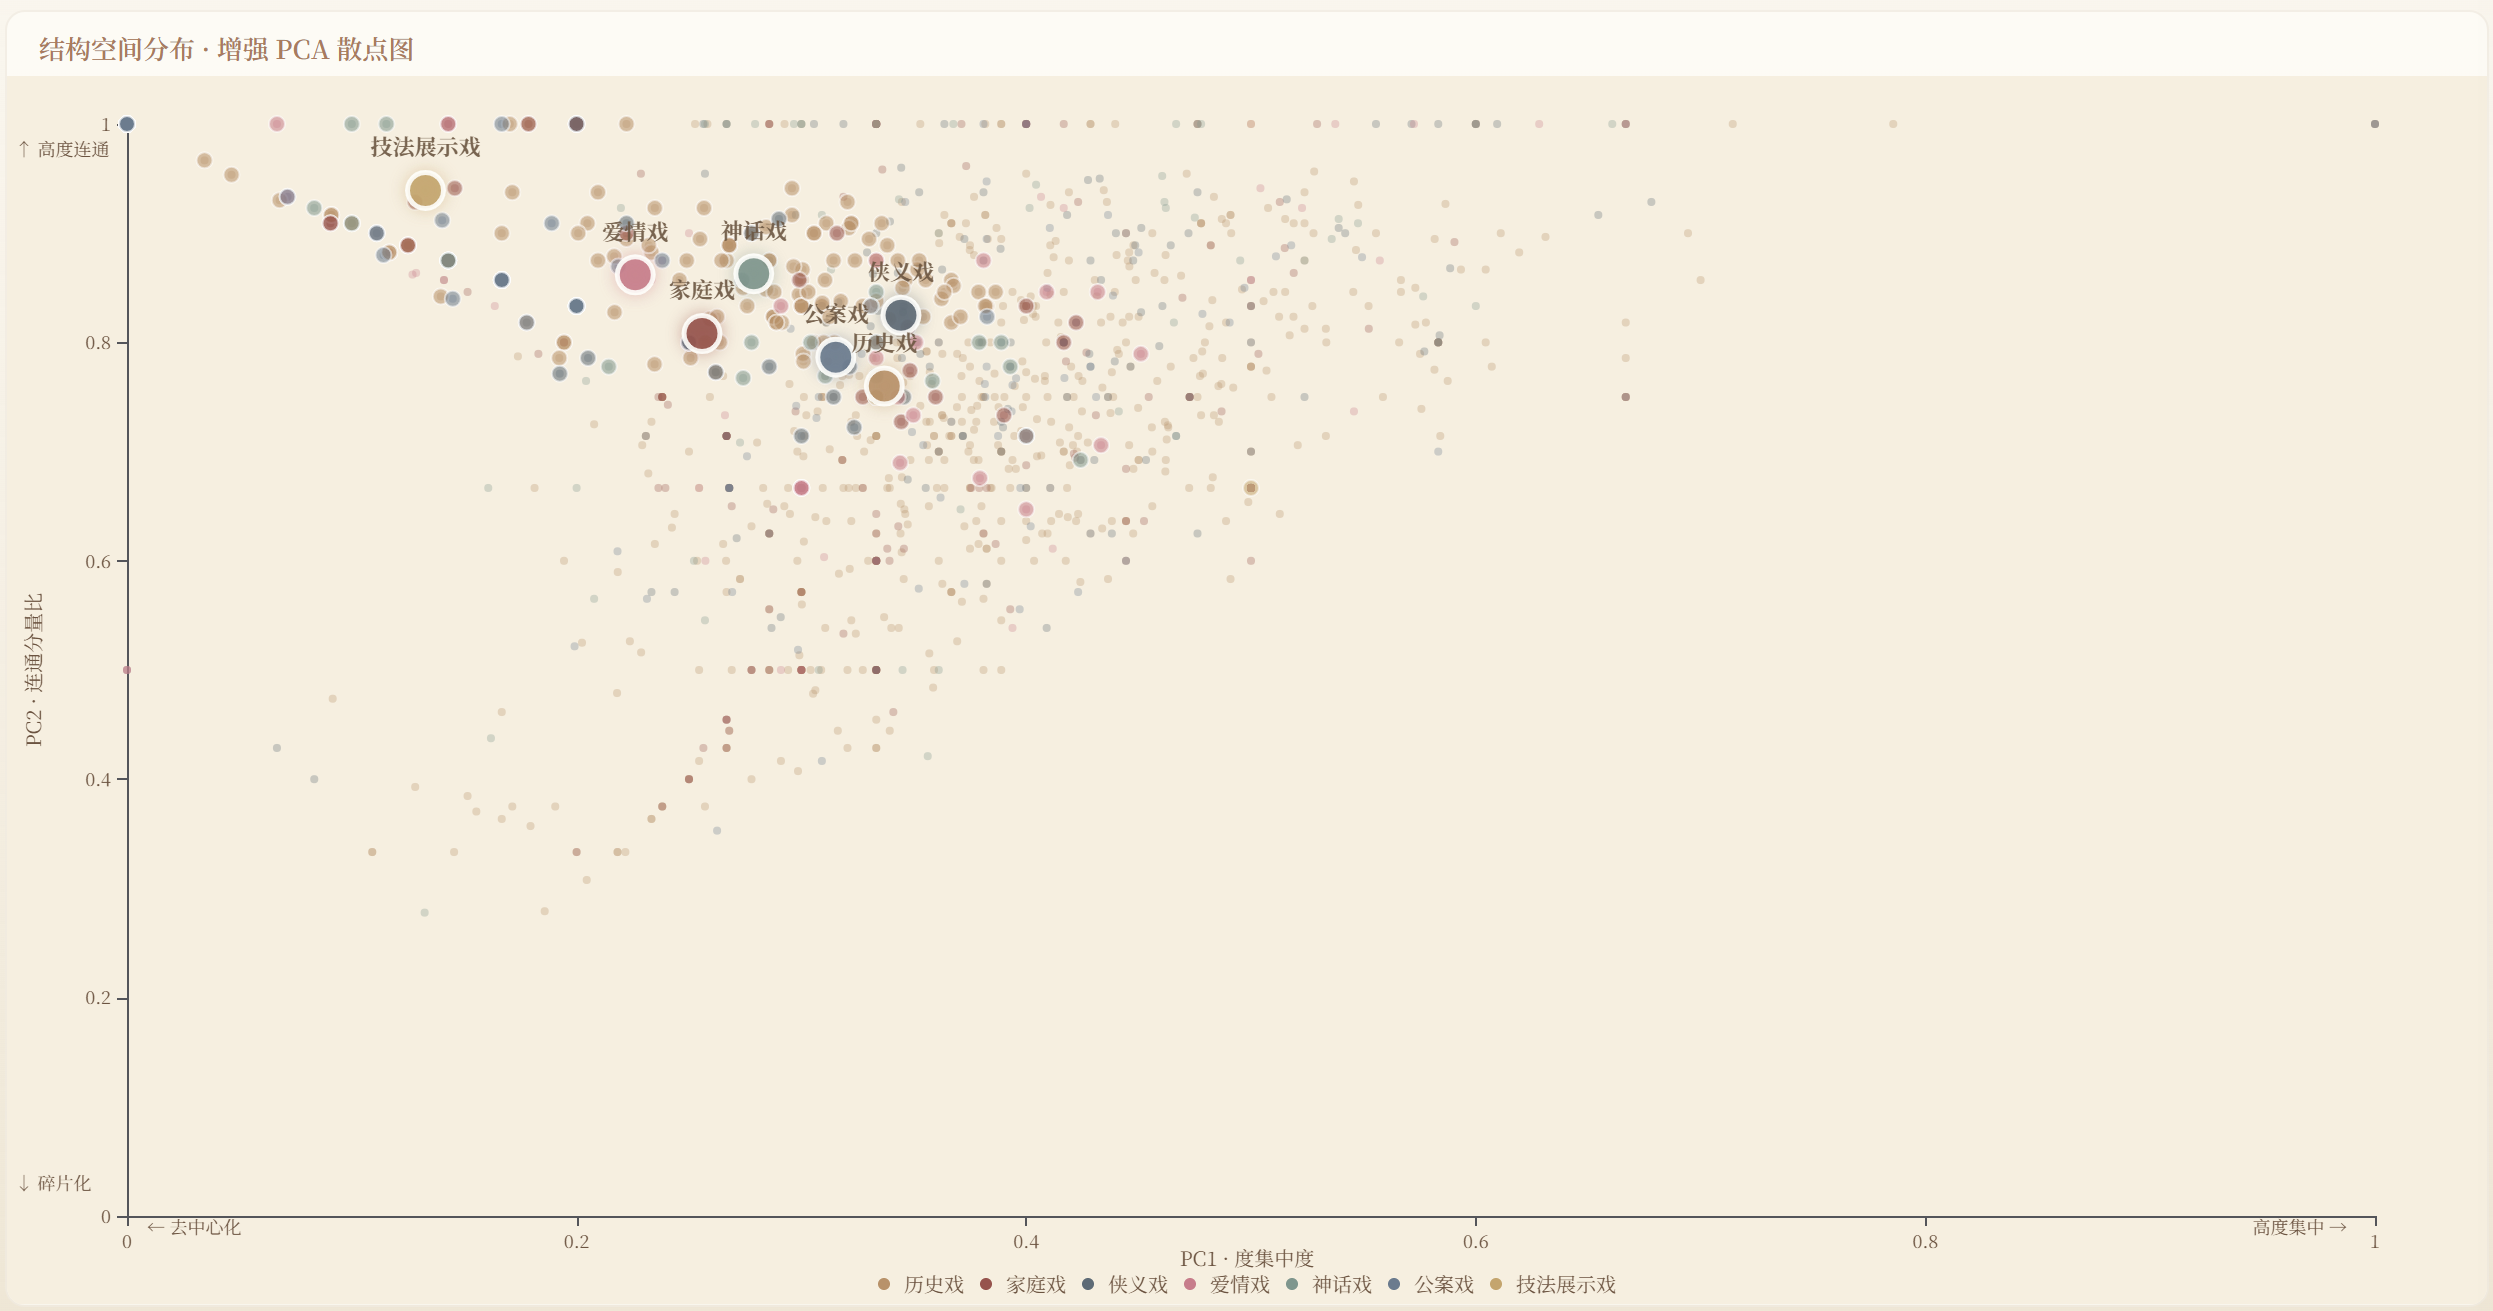
\includegraphics[width=1.0\textwidth]{Image/q2-3-space-map.png}
\caption{图2.2 七类剧目在结构空间中的分布}
\end{figure}

{\fontsize{12bp}{20bp}\kaishu
以《走麦城（一名：麦城升天）》为例（图2.3），这一版网络包含 56 个角色、223 条边，关羽处于明显中心位置：内层是与关平的亲属联系，周仓、廖化、王甫、马良等构成从属或同盟圈层，外围则分布着徐晃、曹仁、吕常、孙权、吕蒙等对峙角色。这个个案把亲属、部属与战场对抗交织在同一张网中，和历史戏常见的“核心人物 + 随从体系 + 阵营博弈”结构十分接近。
}

% ================= 图2.3：单剧个案拼图 =================
% 文件存放位置：Image/q2-3-play-case-zoumaicheng-collage.png
% 图片内容：左图使用《走麦城》角色关系网络，右图使用同一剧目的互动剖面图（建议选择情感-频次象限图，若信息过密可改为互动频次排名图）
% 使用方法：图片准备好后，取消下方 figure 注释即可
% 截图要求：只截取图表主体，不截页面文字说明；左图建议关闭中立边或尽量突出亲属/从属/敌对三类边
%
\begin{figure}[H]
\centering
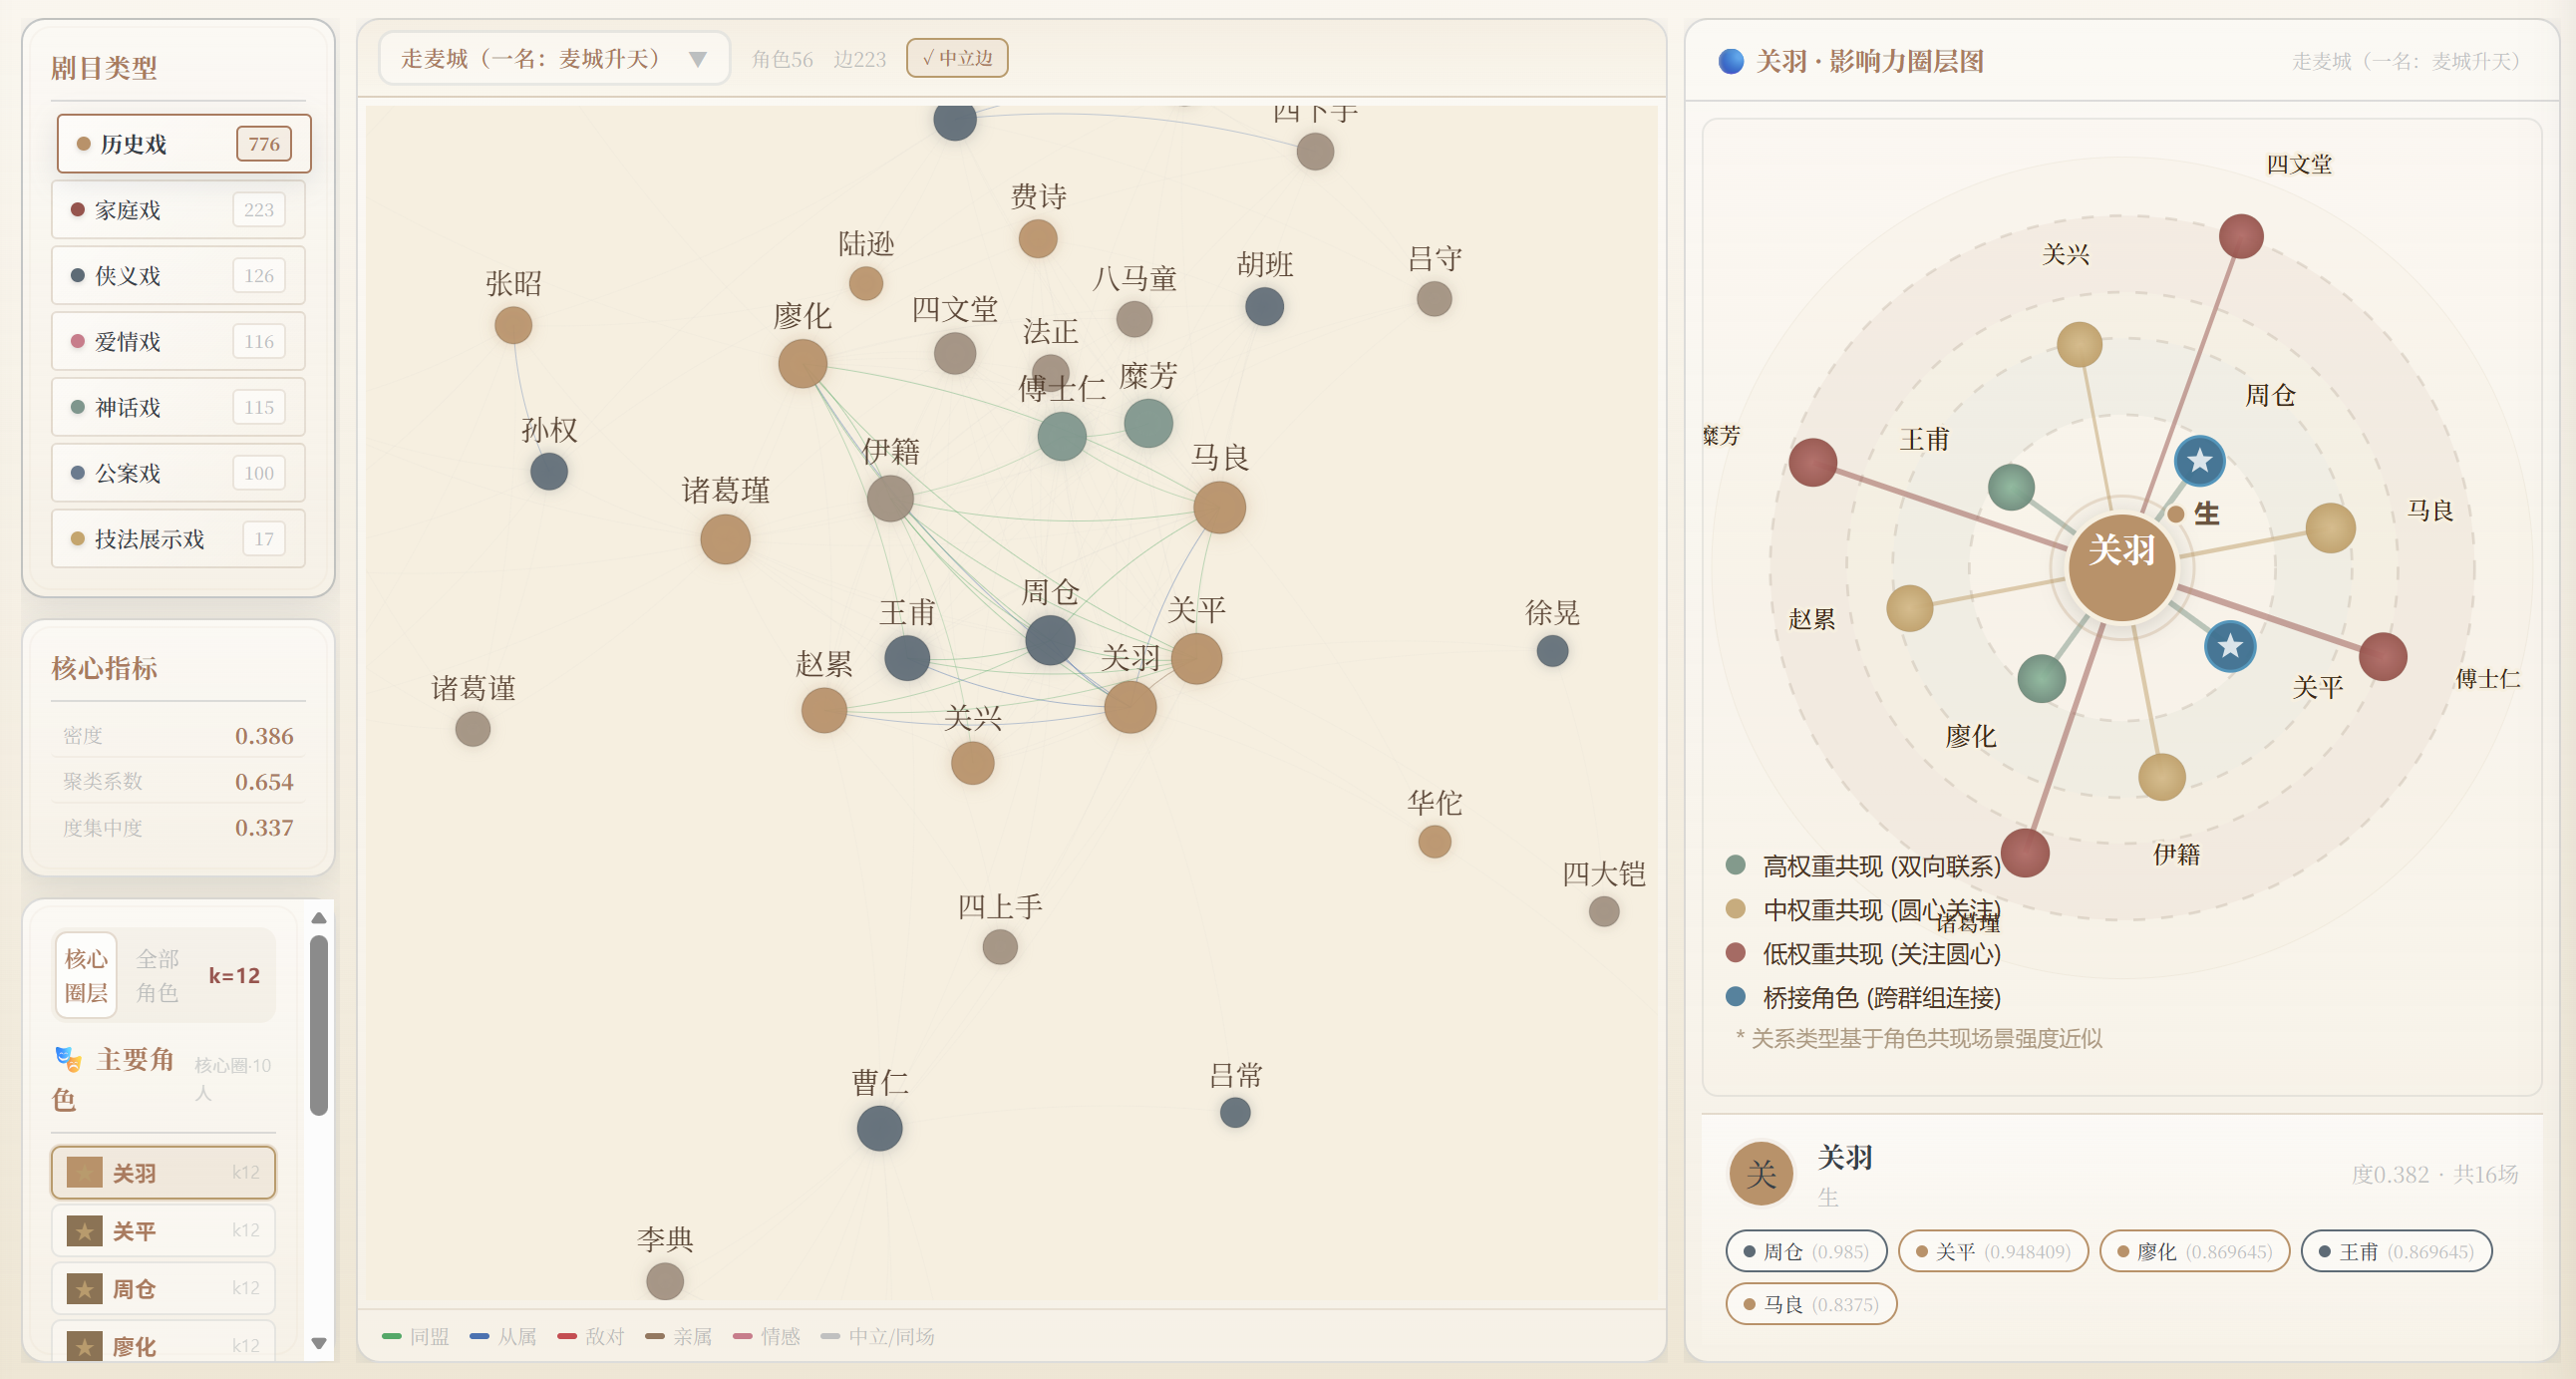
\includegraphics[width=1.0\textwidth]{Image/q2-3-play-case-zoumaicheng-collage.png}
\caption{图2.3 《走麦城》中的角色关系个案}
\end{figure}

{\fontsize{13bp}{18bp}\heiti\bfseries 2.4 综合判断}

\vspace{4pt}

{\fontsize{12bp}{20bp}\kaishu
综合来看，角色关系网络不仅能够在 1{,}473 部剧本中稳定构建，也能回到单部剧本中得到验证；不同剧目确实对应着不同的关系组织方式，历史戏更像阵营分明的群像战场，家庭戏更像互动紧密的亲缘团块，爱情戏更像围绕核心人物收束的双核网络，侠义、公案、神话和技法展示戏也各有稳定而可辨认的结构特征。因此，角色关系网络并不是附属信息，而是区分剧目类型的一项重要结构证据。
}

\vspace{10pt}

\newpage

% ============================================================
% 问题三
% ============================================================

{\fontsize{13bp}{20bp}\heiti\bfseries
3、请从剧本中提取核心主题，分析不同剧本的主题构成及其组合方式。通过跨剧本比较，总结主题表达的共性与差异，探讨是否存在具有代表性的主题组合模式及其特征。
}

\vspace{6pt}

{\fontsize{13bp}{18bp}\heiti\bfseries 3.1 主题提取方式与整体特征}

\vspace{4pt}

{\fontsize{12bp}{20bp}\kaishu
我们先从 1{,}473 部剧本的情节摘要中提取 12 维主题向量，再统计各主题在不同剧目中的覆盖率、共现关系和组合频次，并结合卡方检验、NPMI 共现分析与类型相似度比较，观察京剧主题表达的共性、差异和稳定组合模式。
}

{\fontsize{12bp}{20bp}\kaishu
从整体比较结果看，我们发现 12 个主题都与剧目类型显著相关（p<0.01）；同时，在 1{,}423 部存在激活主题的剧本中，还可以识别出较稳定的主题组合结构。这说明京剧主题既有跨类型共享的基础层，也有能够区分剧目类型的主题指纹。
}

\vspace{6pt}

{\fontsize{13bp}{18bp}\heiti\bfseries 3.2 主题覆盖率中的共性与分化}

\vspace{4pt}
{\fontsize{12bp}{20bp}\kaishu
\begin{itemize}[leftmargin=2.2em,itemsep=2pt,topsep=2pt]
\item \textbf{基础主题}：家庭伦理（58.9\%）和宫廷朝堂（57.4\%）覆盖率最高，生死离别（47.0\%）次之。这三类主题在多种剧目中都会反复出现，构成京剧最普遍的叙事底色。
\item \textbf{历史戏指纹}：宫廷朝堂、征战讨伐、智谋韬略更集中于历史戏，其中历史戏中宫廷朝堂覆盖率达 64.0\%，征战讨伐达 56.9\%。
\item \textbf{类型区分主题}：神话灵异最能区分神话戏，在神话戏中的覆盖率达 83.2\%；冤案昭雪最能区分公案戏，在公案戏中的覆盖率达 80.2\%；侠义江湖则最偏向侠义戏，覆盖率为 62.3\%；爱情姻缘在爱情戏中的覆盖率为 43.7\%。
\end{itemize}
}

\vspace{6pt}

{\fontsize{12bp}{20bp}\kaishu
如果进一步看统计检验结果：
\begin{itemize}[leftmargin=2.2em,itemsep=2pt,topsep=2pt]
\item 神话灵异的区分度最高，\ensuremath{\chi^2}=370.41；
\item 征战讨伐次之，\ensuremath{\chi^2}=221.45；
\item 忠义报国最低，\ensuremath{\chi^2}=18.56。
\end{itemize}
}

% ================= 图3.1：类型×主题拼图 =================
% 文件存放位置：Image/q3-2-theme-structure-collage.png
% 图片内容：左图使用“剧目类型分布”柱状图；右图使用“类型×主题交叉”气泡矩阵
% 使用方法：图片准备好后，取消下方 figure 注释即可
% 截图要求：只截图图表主体；柱状图需保留全部12个主题标签与类型图例，气泡矩阵需保留全部12个主题与7类剧目
%
\begin{figure}[H]
\centering
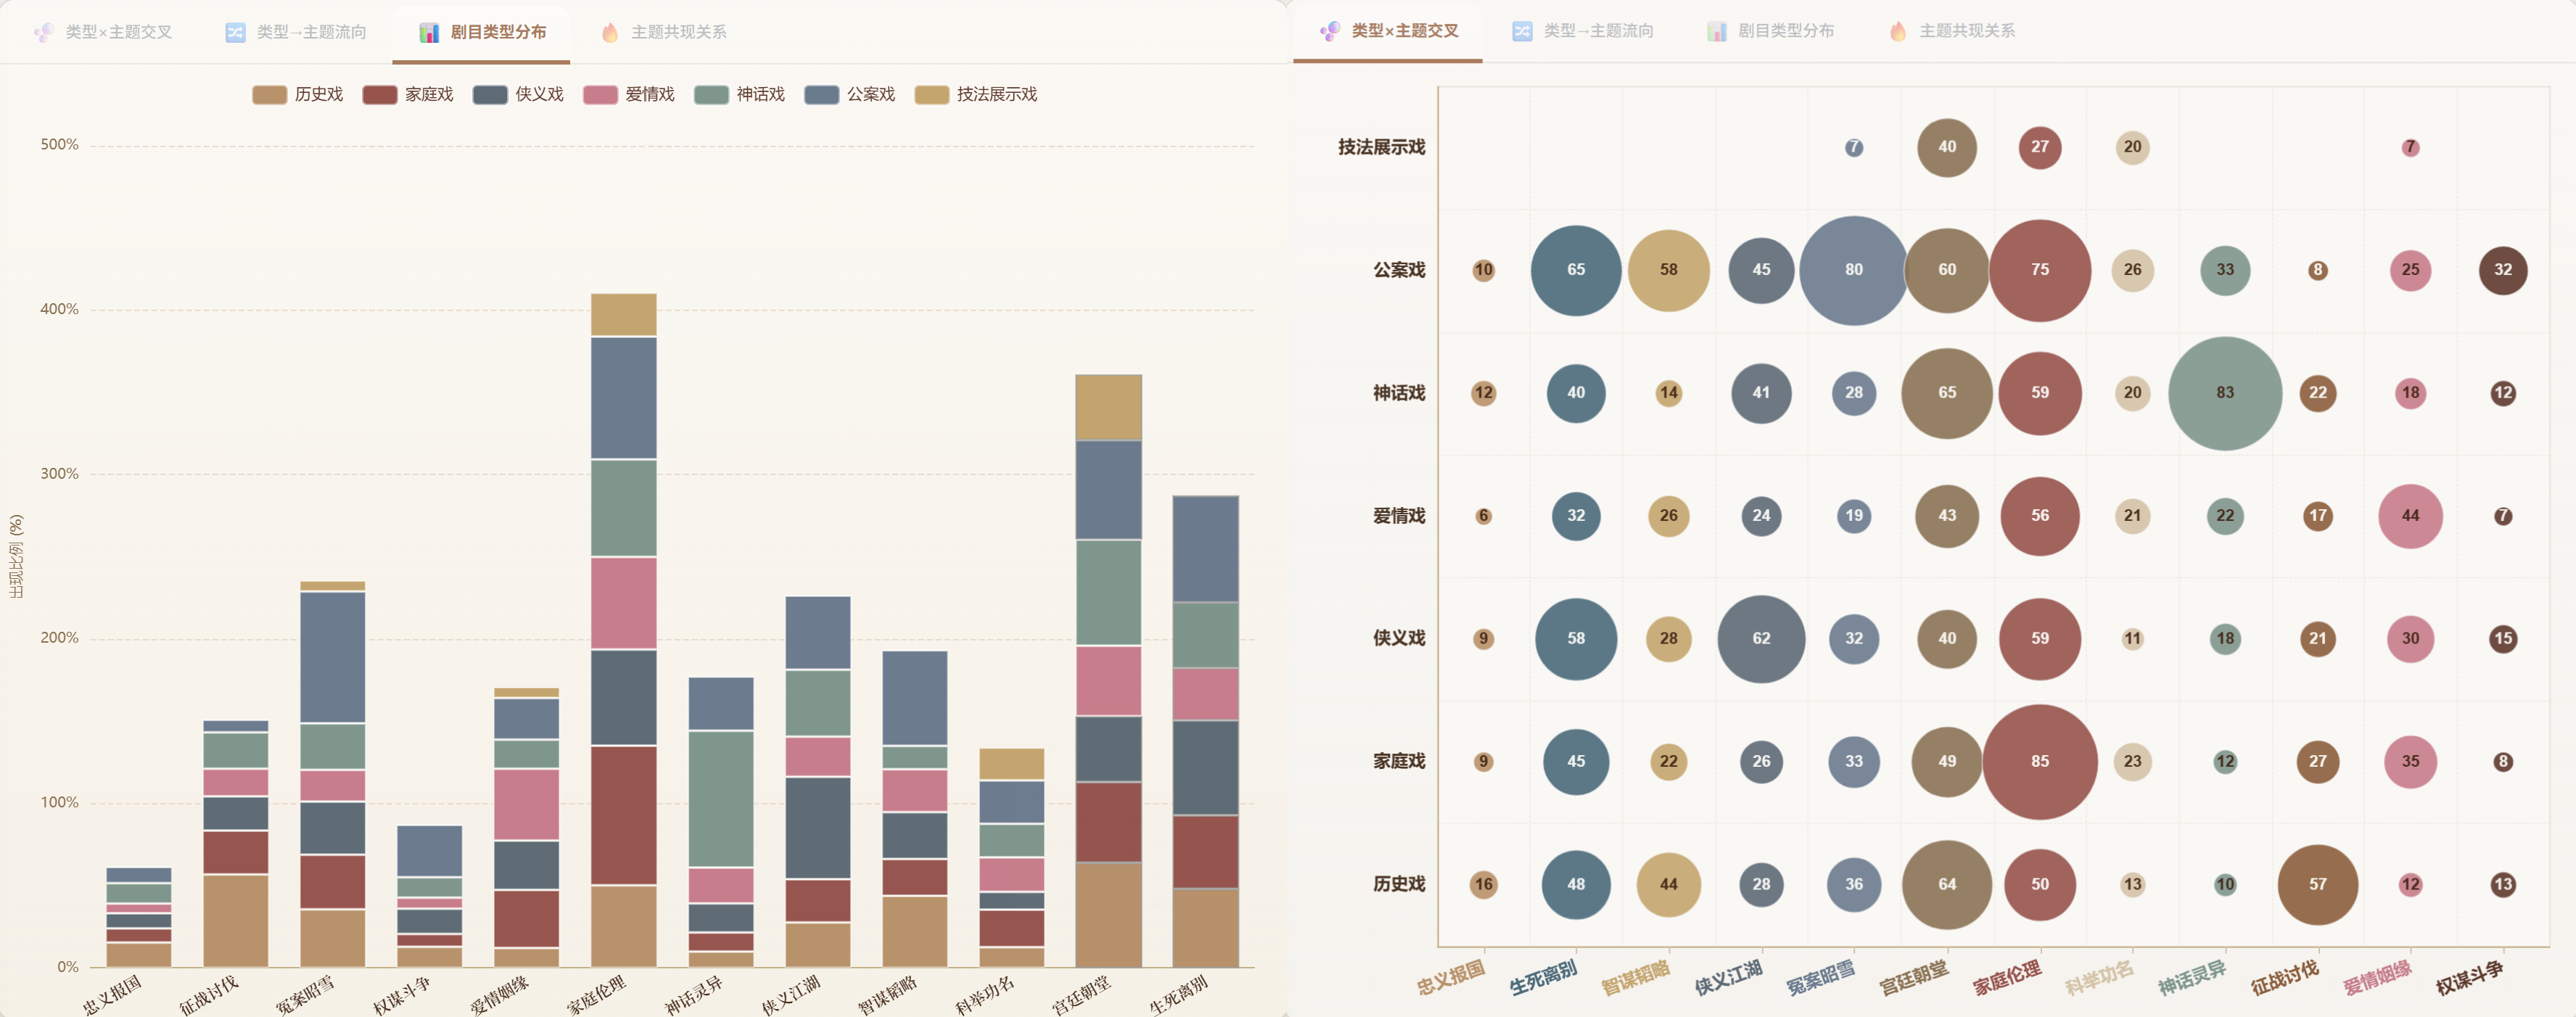
\includegraphics[width=0.87\textwidth]{Image/q3-2-theme-structure-collage.png}
\caption{图3.1 不同剧目类型的主题构成差异}
\end{figure}

\vspace{6pt}

{\fontsize{12bp}{20bp}\kaishu
结合图 3.1 可以更直观看到，“神话灵异”和“征战讨伐”更适合区分剧目类型，而“忠义报国”则更接近覆盖率较低、类型区分度也相对有限的弱区分主题。
}

% \vspace{6pt}

{\fontsize{13bp}{18bp}\heiti\bfseries 3.3 高频共现背后的组合原型}

% \vspace{4pt}

{\fontsize{10.5bp}{15bp}\selectfont
\renewcommand{\arraystretch}{1.24}
\begin{center}
\begin{tabular}{C{0.18\textwidth} L{0.29\textwidth} C{0.16\textwidth} L{0.21\textwidth}}
\toprule
原型 & 核心主题组合 & 主导剧种 & 说明 \tabularnewline
\midrule
宫廷权谋型 & 宫廷朝堂 + 权谋斗争 / 智谋韬略 & 历史戏、公案戏 & 以朝堂博弈、政治冲突和谋略运作为中心 \tabularnewline
家庭伦理型 & 家庭伦理 + 生死离别 & 家庭戏、爱情戏 & 亲情、伦理与离散悲欢共同推动叙事 \tabularnewline
征战智略型 & 征战讨伐 + 智谋韬略 & 历史戏 & 战争推进与谋略布局同时占主导 \tabularnewline
侠义公案型 & 侠义江湖 + 冤案昭雪 & 侠义戏、公案戏 & 以伸冤、救助、惩恶为核心冲突 \tabularnewline
神话灵异型 & 神话灵异 + 宫廷朝堂 & 神话戏 & 超自然叙事常与天庭、人间秩序并置 \tabularnewline
才子佳人型 & 爱情姻缘 + 科举功名 & 爱情戏、家庭戏 & 爱情线与功名线交织出现 \tabularnewline
\bottomrule
\end{tabular}
\end{center}
}

{\fontsize{12bp}{20bp}\kaishu
从共现数量看，“宫廷朝堂 + 家庭伦理”共现 520 部，是最常见的主题组合；“家庭伦理 + 生死离别”共现 471 部，说明家庭叙事经常与离别、失落等情绪主题绑定出现。从关联强度看，NPMI 最高的主题对是“智谋韬略 $\leftrightarrow$ 权谋斗争”（+0.26），说明在出现“权谋斗争”时，往往也会同时出现较强的智略表达（图3.2）。
}

% \vspace{6pt}

% ================= 图3.2：组合模式拼图 =================
% 文件存放位置：Image/q3-3-combo-pattern-collage.png
% 图片内容：左图使用“主题-剧目类型二部图”；右图使用“主题组合原型”和“主题丰度”卡片区域
% 使用方法：图片准备好后，取消下方 figure 注释即可
% 截图要求：不截文字说明板块；二部图需保留主要连线关系；右侧需保证六类原型名称、数量和主题丰度指标清晰可读
%
\begin{figure}[H]
\centering
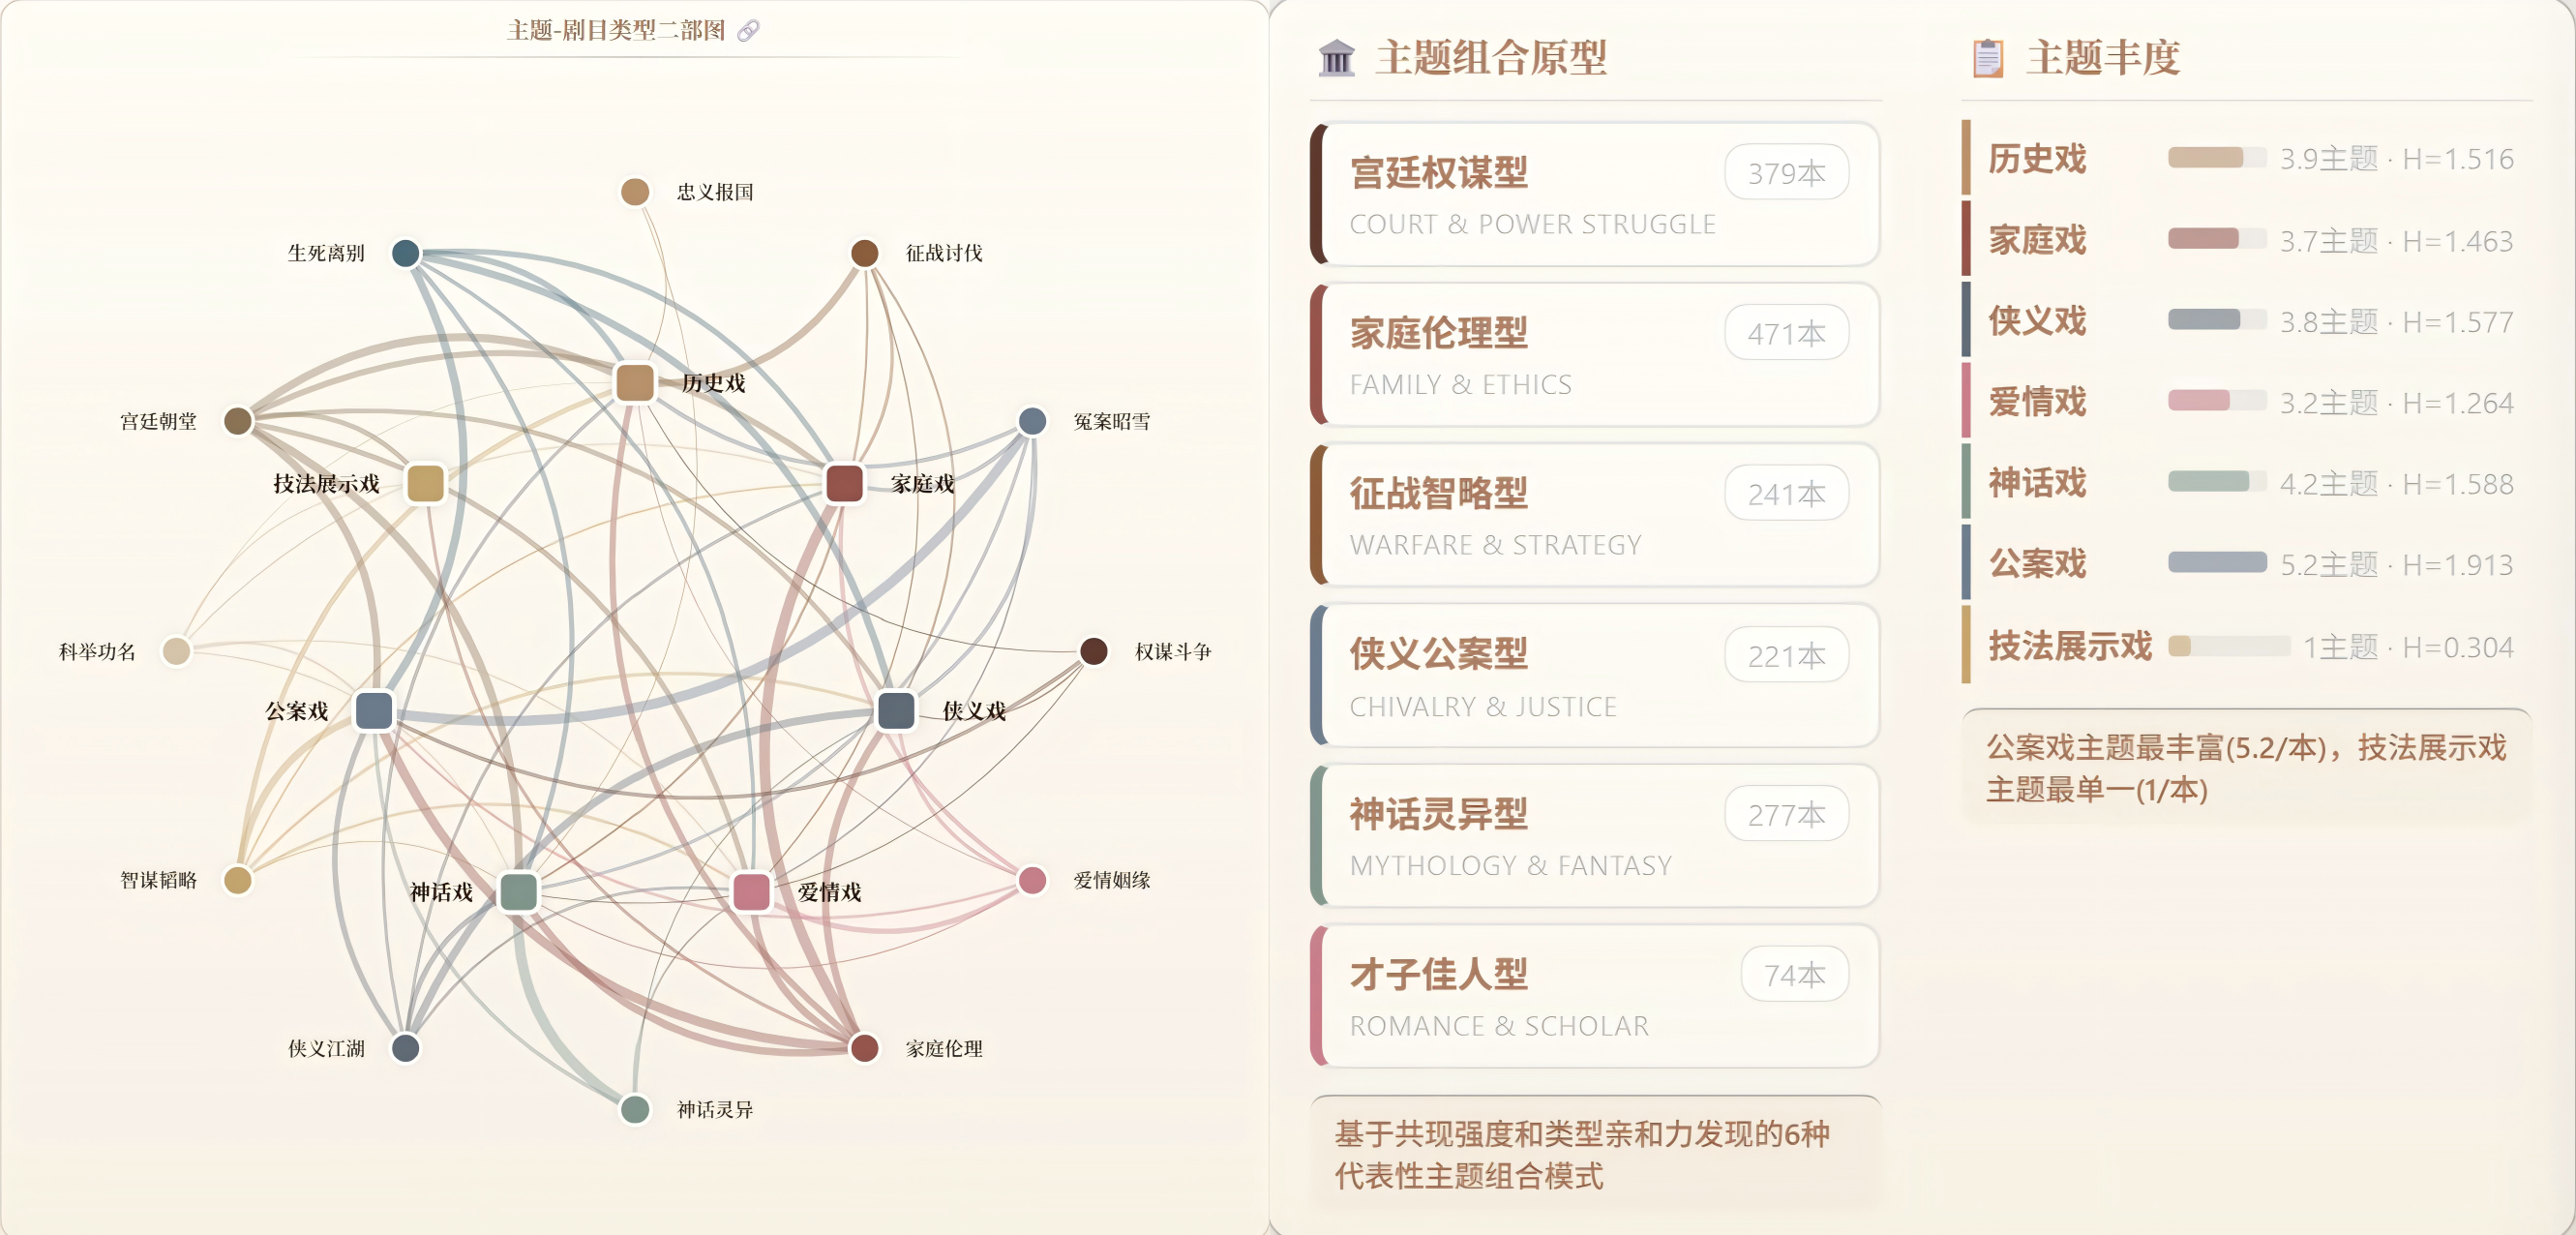
\includegraphics[width=0.80\textwidth]{Image/q3-3-combo-pattern-collage.png}
\caption{图3.2 京剧剧本中的代表性主题组合模式}
\end{figure}

{\fontsize{13bp}{18bp}\heiti\bfseries 3.4 跨剧本比较中的接近与分离}

% \vspace{4pt}

{\fontsize{12bp}{20bp}\kaishu
跨剧本比较后，有两层规律比较清楚：
\begin{enumerate}[leftmargin=2.2em,itemsep=2pt,topsep=2pt]
\item \textbf{相近剧种会共享主题底色}：家庭戏与爱情戏的主题距离最小，约为 0.033，说明它们在家庭伦理、爱情姻缘、生死离别等方面高度接近。
\item \textbf{边缘剧种会拉开明显差异}：技法展示戏与其他类型的主题距离普遍较大，其中与侠义戏距离最大（0.436），说明它更偏向表演展示，主题复合度明显弱于完整叙事剧本。
\end{enumerate}
}

{\fontsize{12bp}{20bp}\kaishu
回到具体剧目，以《过五关（一名：辞曹斩将）》为例（图3.3），其最突出的单一主题是冤案昭雪，宫廷朝堂次之，征战讨伐与智谋韬略也占有一定比重；整体上更接近历史戏中常见的复合结构，而不是单一的忠义主题。这说明同一人物形象进入不同剧本后，仍然会受到剧目整体主题结构的制约。
}

% ================= 图3.3：单剧主题个案图 =================
% 文件存放位置：Image/q3-4-play-case-guowuguan.png
% 图片内容：使用单剧本模式下《过五关（一名：辞曹斩将）》的主题结构页，保留左侧单剧主题关系图与右侧六维雷达图
% 使用方法：图片准备好后，取消下方 figure 注释即可
% 截图要求：保留标题区、左侧主题关系图和右侧雷达图，不截下方大段说明文字；若单图信息不足，可与一句正文配合使用
%
\begin{figure}[H]
\centering
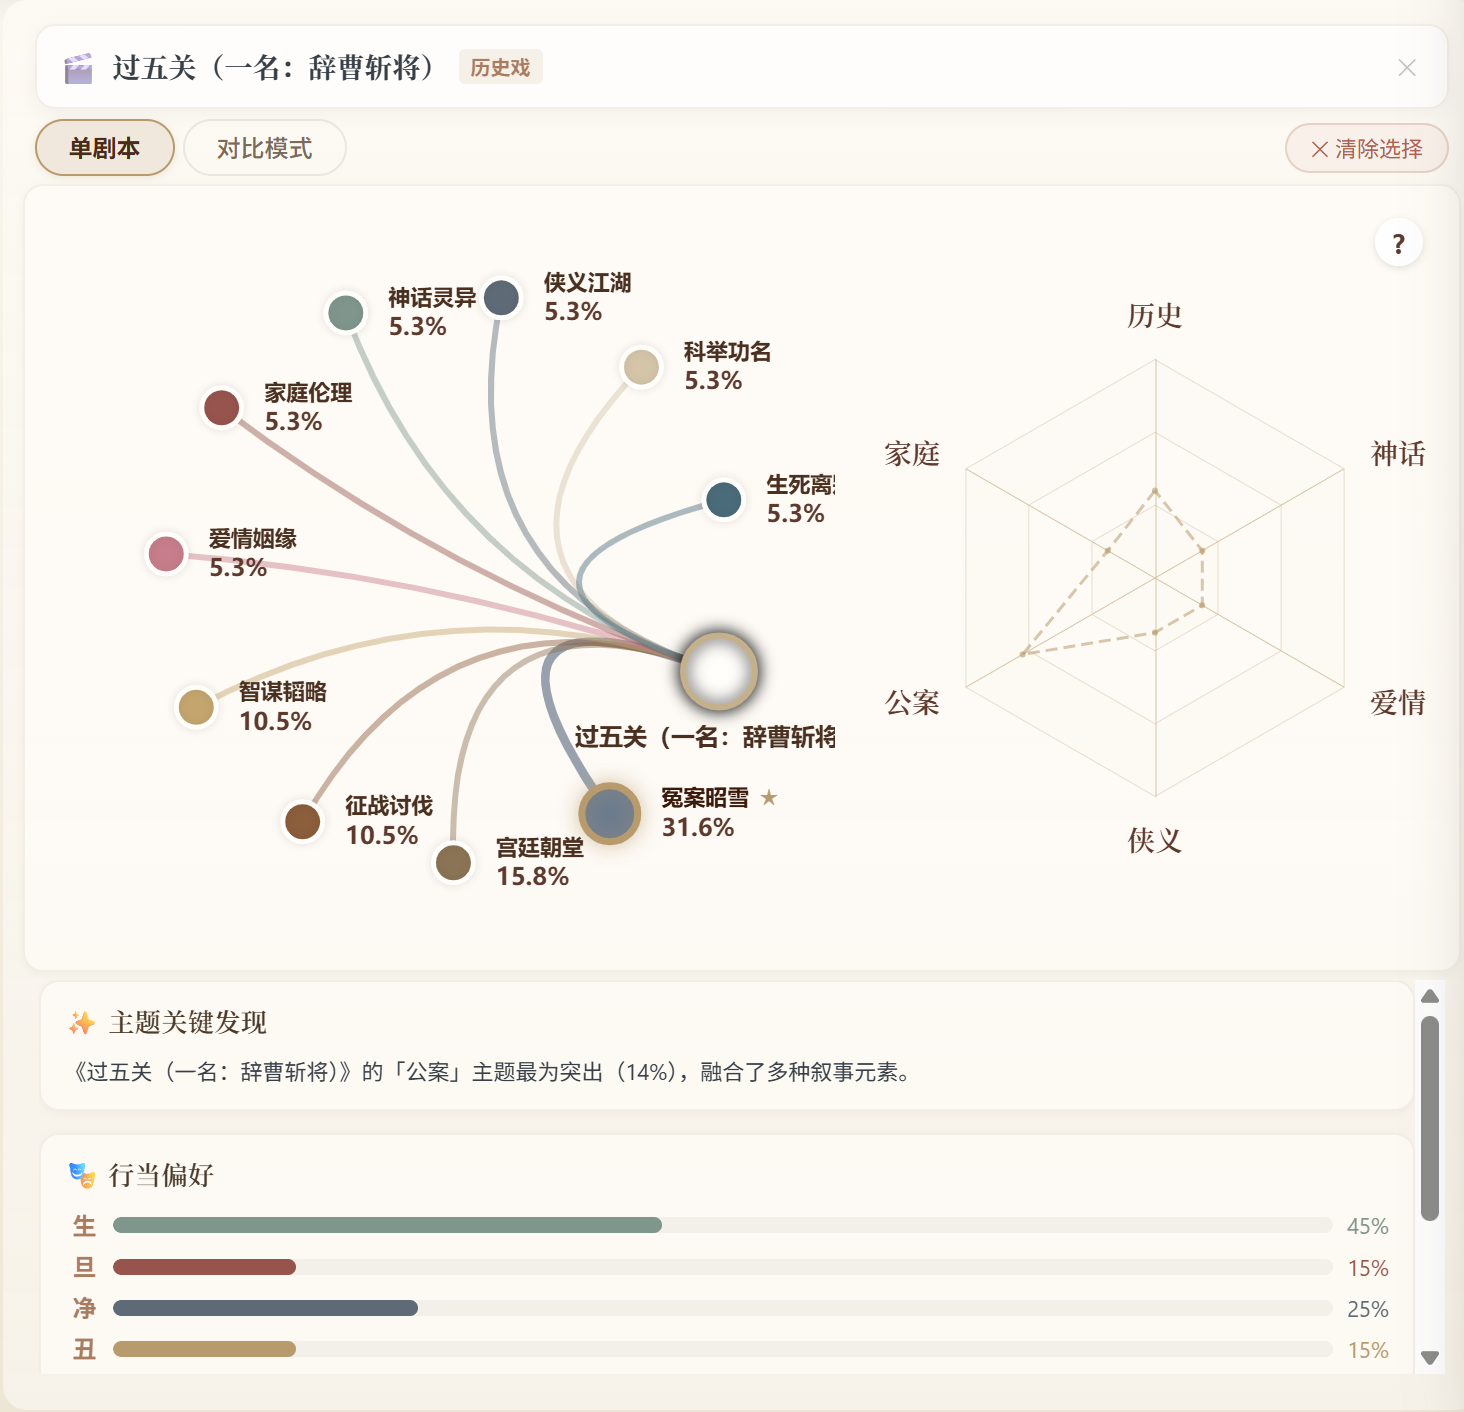
\includegraphics[width=0.75\textwidth]{Image/q3-4-play-case-guowuguan.png}
\caption{图3.3 《过五关》中的主题构成个案}
\end{figure}

{\fontsize{13bp}{18bp}\heiti\bfseries 3.5 综合判断}

% \vspace{4pt}

{\fontsize{12bp}{20bp}\kaishu
综合来看，我们认为京剧剧本存在比较稳定的核心主题体系，其中家庭伦理、宫廷朝堂、生死离别构成最普遍的基础层；不同剧目又会围绕征战讨伐、冤案昭雪、侠义江湖、神话灵异、爱情姻缘等优势主题形成各自的表达重心；再往下看，还可以进一步整理出六种较清晰的主题组合原型。因此，京剧主题表达既有共性，也有可辨认的类型差异。
}

% \vspace{10pt}

% ============================================================
% 问题四
% ============================================================

{\fontsize{13bp}{20bp}\heiti\bfseries
4、请基于剧本中表演形式的标记以及剧本内容等对剧本的叙事结构进行系统分析，识别剧情发展中的关键阶段，刻画剧情起伏与节奏变化。进一步比较不同剧本在叙事结构上的差异，总结典型叙事模式及其结构特征。
}

\vspace{6pt}

{\fontsize{13bp}{18bp}\heiti\bfseries 4.1 叙事曲线提取与整体节奏}

\vspace{4pt}

{\fontsize{12bp}{20bp}\kaishu
我们先从 1{,}473 部剧本中提取逐场冲突值、情感值和角色密度，形成单剧叙事曲线；再结合唱、念、白、打等表演形式比例，对单剧进行阶段切分，并对全量剧本做模式归纳。由于 291 部单场戏难以形成完整的前后段结构，因此在讨论高潮位置时，以 1{,}182 部多场剧本为统计对象；在比较典型模式时，仍使用全部 1{,}473 部剧本。
}

{\fontsize{12bp}{20bp}\kaishu
从整体结果看，我们发现多场剧本的叙事高潮平均落在全剧进程的 34.5\%，整体偏前；这说明京剧往往较早推出关键冲突，再通过后续铺陈、转折与收束完成节奏展开。与此同时，全量剧本还可以整理出 8 种较稳定的叙事模式，其中线性渐进式与史诗铺陈式合计占 47.4\%，构成最主要的两类结构底盘。
}

\vspace{6pt}

{\fontsize{13bp}{18bp}\heiti\bfseries 4.2 多场剧本中的四段推进}

\vspace{4pt}
{\fontsize{12bp}{20bp}\kaishu
\begin{enumerate}[leftmargin=2.2em,itemsep=2pt,topsep=2pt]
\item \textbf{开端}：交代人物关系与事件背景，先把核心矛盾推出场面。
\item \textbf{发展}：角色逐步聚拢，冲突与情绪持续累积，是全剧张力上升最快的部分。
\item \textbf{高潮}：主冲突峰值或关键反转出现，往往伴随局部角色密度抬升或表演强度集中。
\item \textbf{结局}：冲突回落，情绪沉淀，人物退出，最后形成道德判断、情感余韵或场面收束。
\end{enumerate}
}

% ================= 图4.1：单剧节奏主图 =================
% 文件存放位置：Image/q4-1-single-rhythm-main.png
% 图片内容：使用单剧本视图中央的 CombinedRhythmChart，展示单剧三层叠加节奏图谱与四阶段背景
% 使用方法：图片准备好后，取消下方 figure 注释即可
% 操作步骤：
% 1. 进入任务四页面，保持左侧“单剧本视图”为选中状态；
% 2. 在左侧剧本列表中搜索并选择《过五关（一名：辞曹斩将）》；
% 3. 截中央主区的大图，只保留三层叠加节奏图谱和阶段背景；
% 截图要求：不要截顶部说明文字、左侧剧本列表和右侧信息栏；优先保证四阶段背景色带、冲突曲线和场次分隔线清晰可见
%
\begin{figure}[H]
\centering
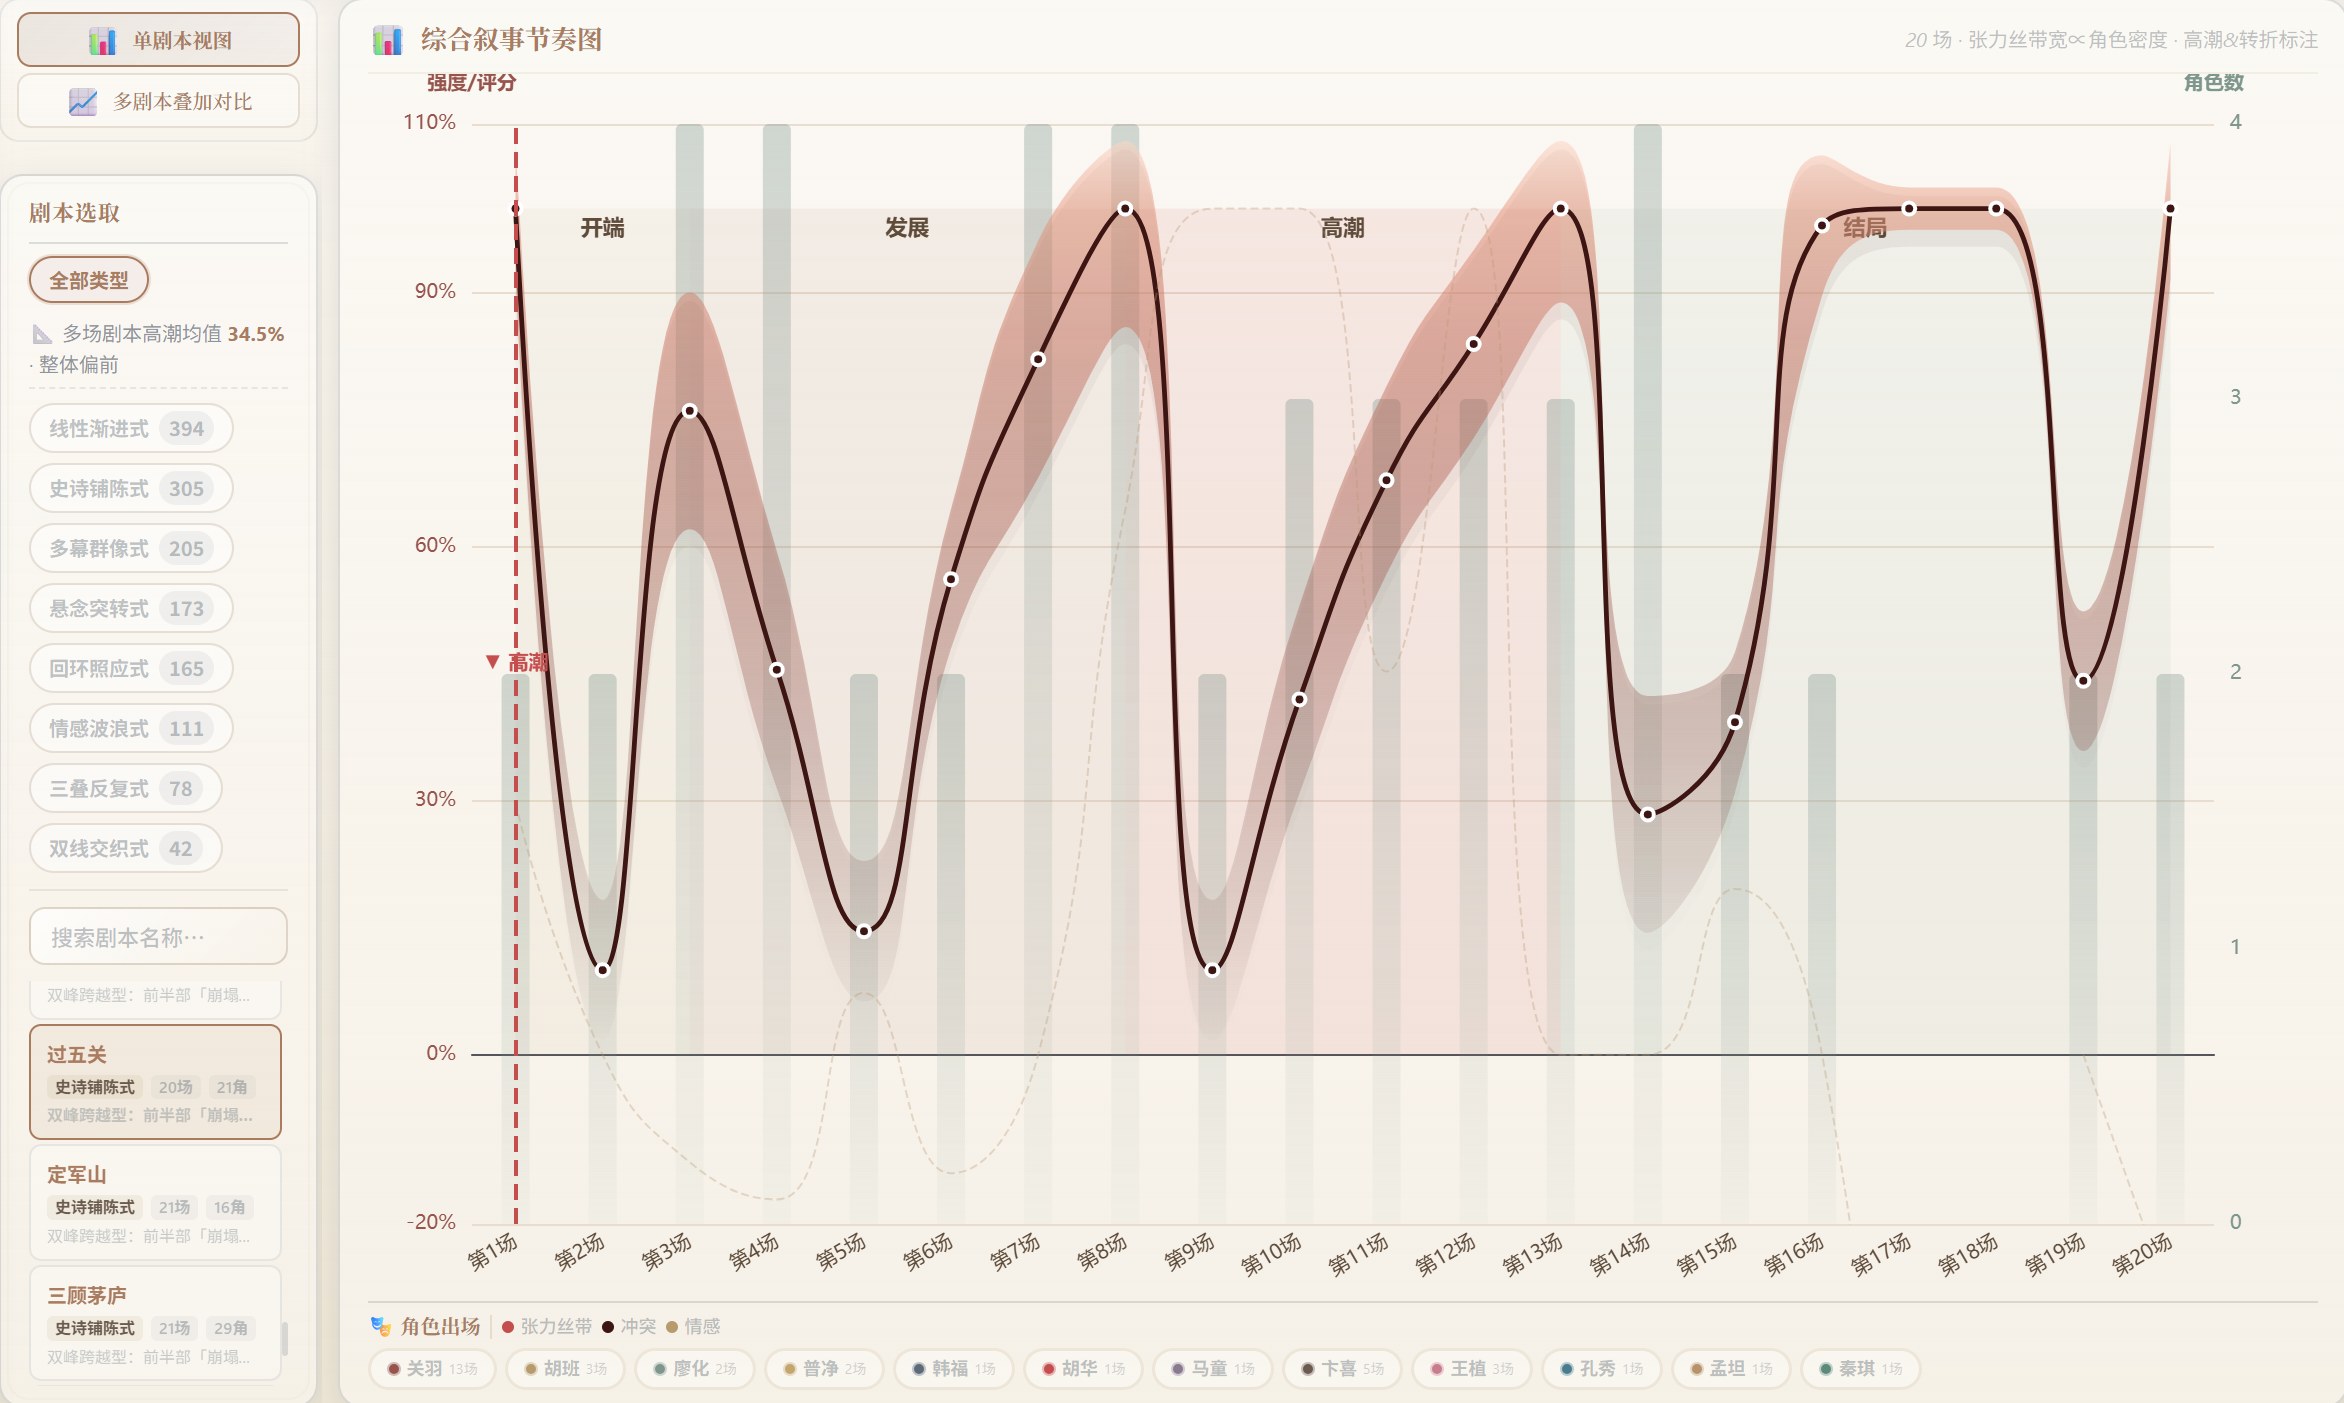
\includegraphics[width=0.75\textwidth]{Image/q4-1-single-rhythm-main.png}
\caption{图4.1 《过五关》单剧叙事结构中的四阶段节奏图}
\end{figure}

{\fontsize{12bp}{20bp}\kaishu
这里的四段划分并不是人工按章回硬分，而是由逐场冲突弧、情感弧和角色密度三条序列联合切分得到；因此它既能落到单部剧本，也能在跨剧本比较中保持统一口径。
}

\vspace{6pt}

{\fontsize{13bp}{18bp}\heiti\bfseries 4.3 高潮位置、节奏差异与表演分工}

\vspace{4pt}
{\fontsize{12bp}{20bp}\kaishu
\begin{enumerate}[leftmargin=2.2em,itemsep=2pt,topsep=2pt]
\item \textbf{高潮整体偏前}：在 1{,}182 部多场剧本中，叙事高潮的平均位置约为全剧进程的 34.5\%。这说明京剧叙事往往会较早推出关键冲突，再通过后续铺陈和转折把张力继续展开。
\item \textbf{剧目越长，高潮越倾向前移}：从多场剧本的整体比较看，场次越多，叙事越需要提前推出主冲突，以便为后续铺陈、转折和收束留出空间。图4.2 中《过五关》《定军山》《三顾茅庐》虽同属史诗铺陈式，但高位波段出现的时机和持续方式并不完全一致，也说明长篇叙事内部仍保留着鲜明的节奏差异。
\item \textbf{表演形式分工清楚}：从 1{,}473 部剧本的整体均值看，白的占比为 61.7\%，唱为 11.9\%，念为 3.8\%，打为 0.9\%。这说明剧情推进主要依靠对白展开，唱段更多承担抒情层次，而打戏虽然占比不高，但更集中承担局部爆发场面。
\end{enumerate}
}

\vspace{6pt}

% ================= 图4.2：多剧本叠加图 =================
% 文件存放位置：Image/q4-2-overlay-compare.png
% 图片内容：使用多剧本视图中央的 MultiPlayOverlayChart，叠加《过五关》《定军山》《三顾茅庐》3 部剧本的冲突曲线，展示同属史诗铺陈式时的节奏差异
% 使用方法：图片准备好后，取消下方 figure 注释即可
% 操作步骤：
% 1. 在左侧切换到“多剧本叠加对比”；
% 2. 在剧本列表里分别勾选《过五关》《定军山》《三顾茅庐》；
% 3. 中央主区会出现多条归一化冲突曲线，直接截取中央主图即可；
% 截图要求：保留图例和曲线，不截左侧长列表；右侧“多剧本对比”统计栏可不截，避免画面过杂
%
\begin{figure}[H]
\centering
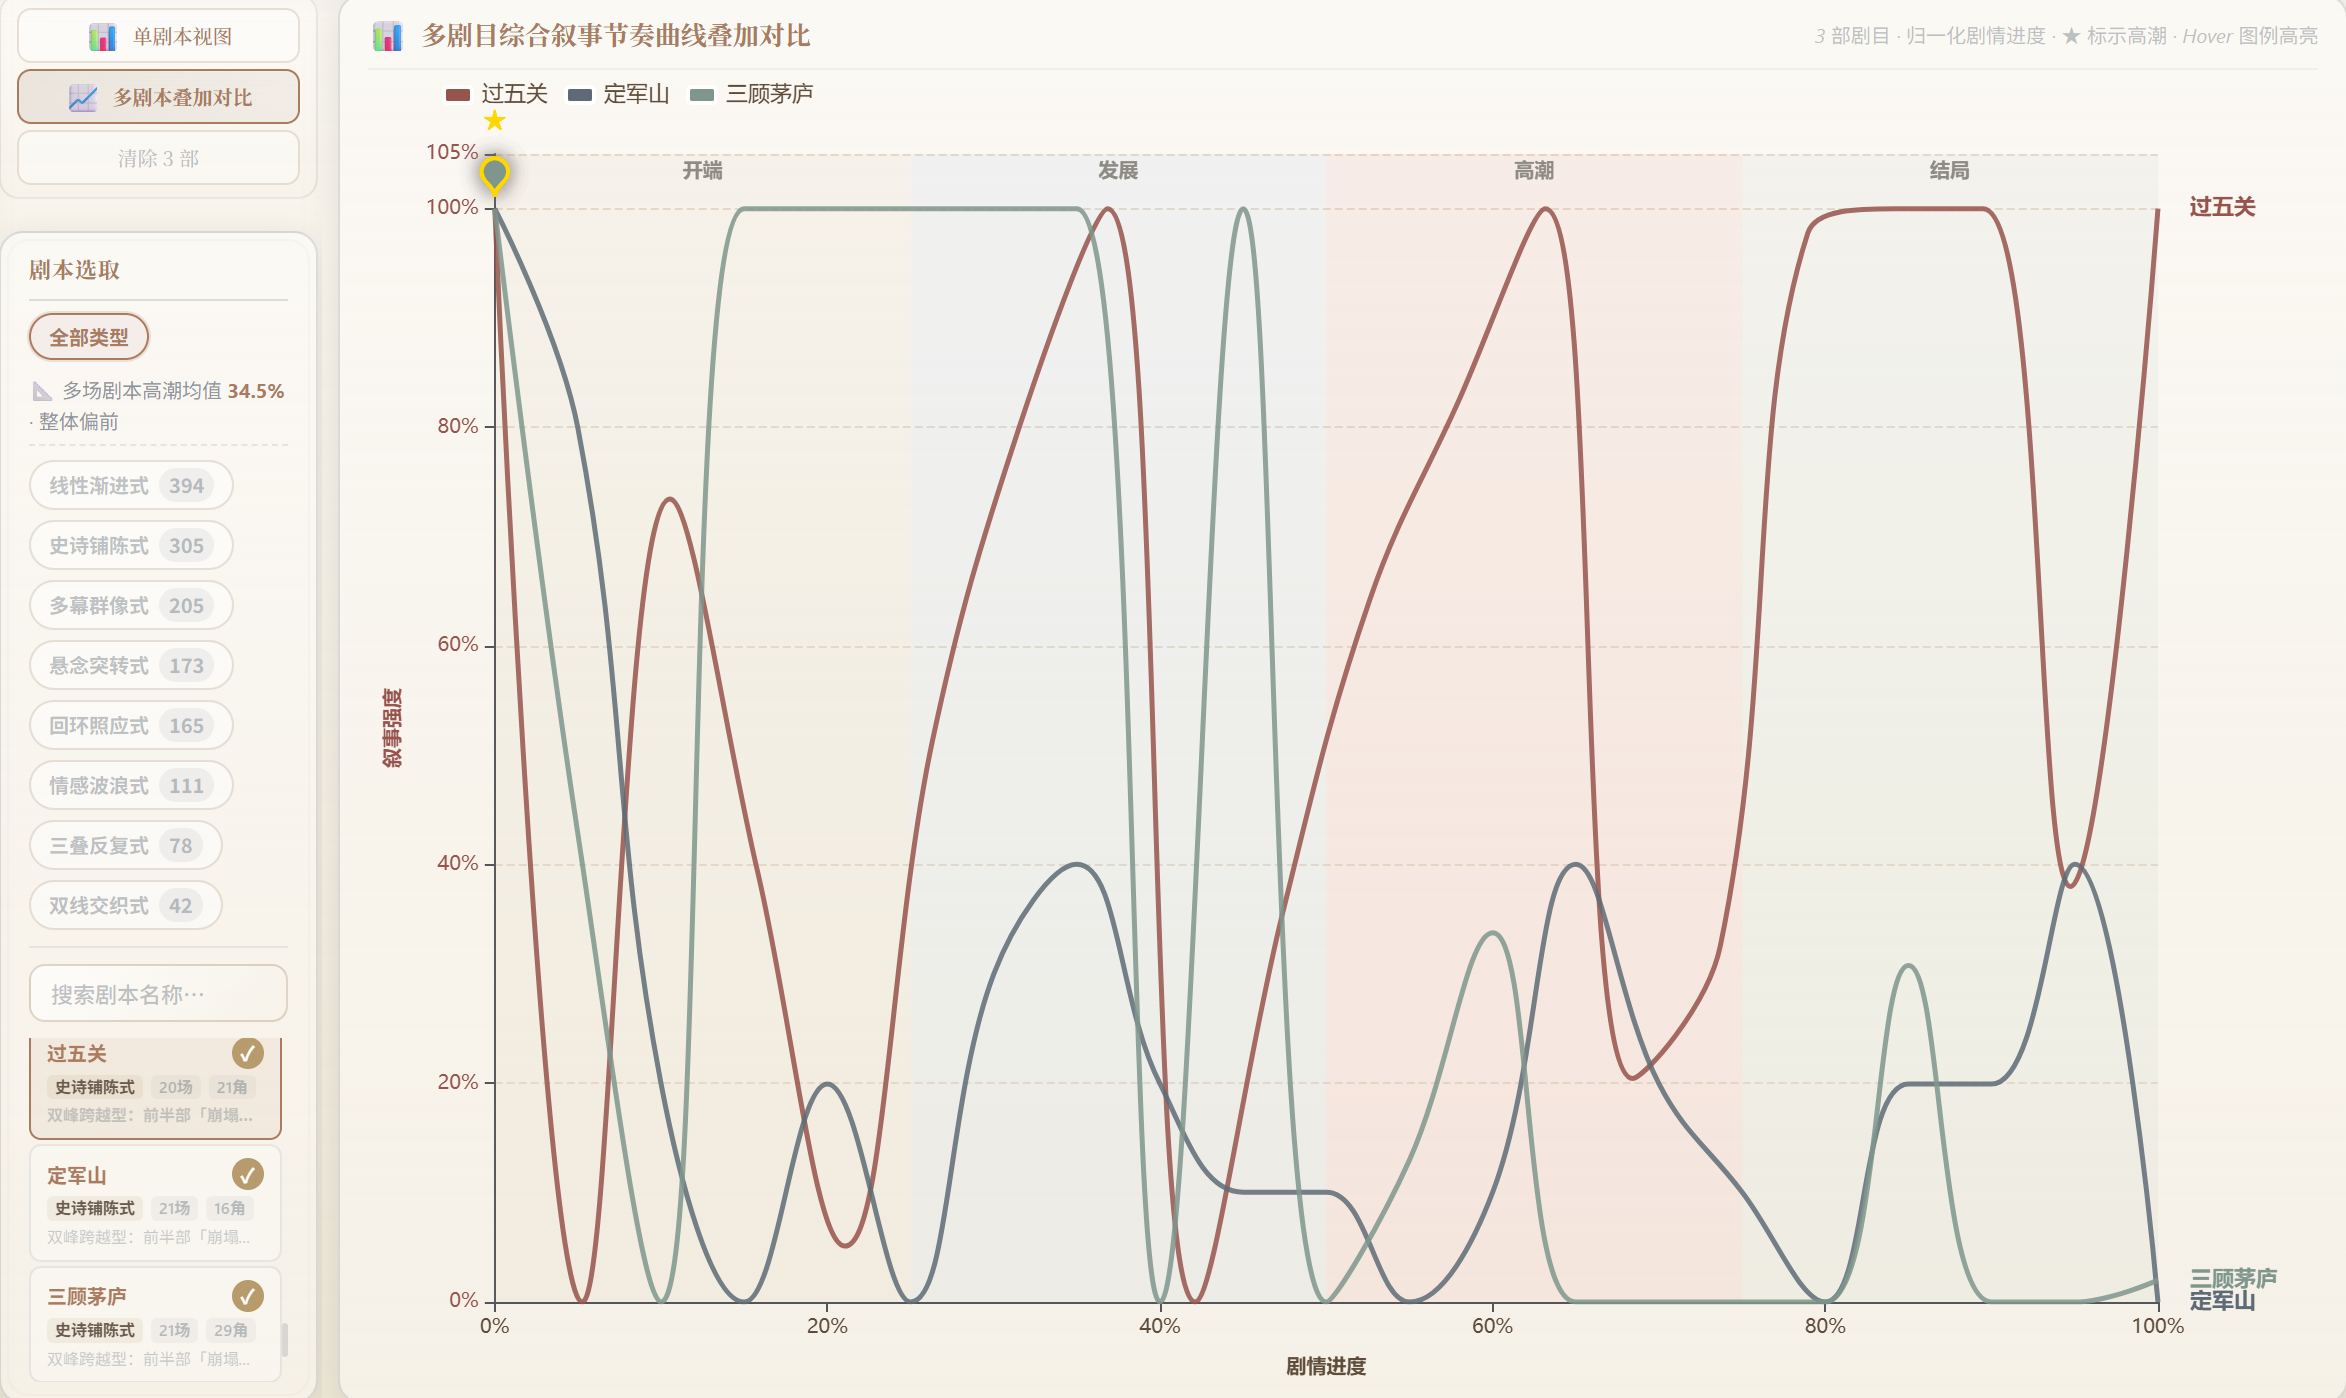
\includegraphics[width=1.0\textwidth]{Image/q4-2-overlay-compare.png}
\caption{图4.2 《过五关》《定军山》《三顾茅庐》的叙事节奏对比}
\end{figure}

{\fontsize{13bp}{18bp}\heiti\bfseries 4.4 八类叙事模式的结构特点}

\vspace{4pt}

{\fontsize{10.5bp}{15bp}\selectfont
\renewcommand{\arraystretch}{1.23}
\begin{center}
\begin{tabular}{C{0.18\textwidth} C{0.12\textwidth} L{0.25\textwidth} L{0.22\textwidth}}
\toprule
模式 & 占比 & 结构特征 & 常见剧目 \tabularnewline
\midrule
线性渐进式 & 26.7\% & 冲突逐场抬升，结构最均衡 & 家庭戏、爱情戏、技法展示戏 \tabularnewline
史诗铺陈式 & 20.7\% & 场次多、人物多，常见多段铺陈 & 历史戏、侠义戏 \tabularnewline
多幕群像式 & 13.9\% & 多角色并进，局部峰值分散 & 历史戏、神话戏 \tabularnewline
悬念突转式 & 11.7\% & 关键节点突然抬升，转折集中 & 历史戏、公案戏、侠义戏 \tabularnewline
回环照应式 & 11.2\% & 首尾呼应，结尾回落到初始情境 & 家庭戏、爱情戏 \tabularnewline
情感波浪式 & 7.5\% & 情绪多波次推进，唱段承载更强 & 家庭戏 \tabularnewline
三叠反复式 & 5.3\% & 相似情境反复升级，节拍清楚 & 短剧、民间小戏 \tabularnewline
双线交织式 & 2.9\% & 两条线并进后汇合，结构最复杂 & 历史戏 \tabularnewline
\bottomrule
\end{tabular}
\end{center}
}

{\fontsize{12bp}{20bp}\kaishu
结合剧目类型来看，历史戏最偏史诗铺陈式（23.7\%）和多幕群像式（15.4\%）；家庭戏、爱情戏和技法展示戏更偏线性渐进式；双线交织式虽然数量最少，但 73.8\% 集中在历史戏中，说明复杂结构主要还是服务于历史群像和多线博弈。
}

\vspace{6pt}

% 任务四仅保留 2 张图。
% “八类典型模式”的证据主要由上表和对应统计结果承担，不再单独配置第 3 张图片。

{\fontsize{13bp}{18bp}\heiti\bfseries 4.5 综合判断}

\vspace{4pt}

{\fontsize{12bp}{20bp}\kaishu
综合来看，我们认为京剧叙事结构并不是平均铺开，而更常较早推出高潮；与此同时，随着剧目篇幅拉长，高潮位置又会相应前移，以便支撑后续更充分的铺陈和收束。在这一总体节奏之下，还可以进一步识别出 8 类典型模式。以《过五关》为例，单剧视图清楚展示了从铺垫、推进到集中爆发再回落收束的完整过程；而与《定军山》《三顾茅庐》的叠加对比，则进一步说明同一模式内部仍存在可辨认的节奏差异。
}

\vspace{10pt}

% ============================================================
% 问题五
% ============================================================

{\fontsize{13bp}{20bp}\heiti\bfseries
5、请在前述分析基础上，综合角色关系、主题结构与叙事结构，系统分析三者之间的关联机制与差异特征。例如，探讨特定角色关系如何承载和推动主题表达，主题结构如何影响叙事策略与剧情组织，以及不同叙事方式又如何重塑角色关系的呈现与演化。通过构建可交互的可视分析系统，探索人物关系、主题表达与叙事方式之间是否存在典型的关联模式、协同演化规律或稳定结构特征。
}

\vspace{6pt}

{\fontsize{13bp}{18bp}\heiti\bfseries 5.1 三类结果的整合与整体关联}

\vspace{4pt}

{\fontsize{12bp}{20bp}\kaishu
把前四问的结果放到同一框架中后，我们可以得到三类可比较特征：第 2 问提供角色网络指标，如网络密度、中心性偏离、聚类系数和角色数量；第 3 问提供 12 维主题向量及 6 类主题簇；第 4 问提供 8 类叙事类型。在此基础上，再依次检验“关系 $\rightarrow$ 主题”“主题 $\rightarrow$ 叙事”“叙事 $\rightarrow$ 关系”三条对应关系，并进一步对 1{,}473 部剧本做综合聚类。
}

{\fontsize{12bp}{20bp}\kaishu
从整体结果看，我们发现三组检验都给出了显著结果；进一步综合网络、主题和叙事特征后，全量剧本还可以收敛为 6 类结构原型。这里更关心的不是某一维单独如何变化，而是三类结构怎样共同组织成可重复的剧本形态，并继续在星图页面中落回到单剧验证。
}

\vspace{6pt}

{\fontsize{13bp}{18bp}\heiti\bfseries 5.2 关系结构与主题容量}

\vspace{4pt}
{\fontsize{12bp}{20bp}\kaishu
\begin{itemize}[leftmargin=2.2em,itemsep=2pt,topsep=2pt]
\item 网络密度与“征战讨伐”显著负相关（点二列相关系数 $r=-0.258$，$p<0.001$），说明战争主题更常出现在关系较疏、阵营较大的剧本中。
\item 角色数量与“侠义江湖”显著正相关（$r=0.231$，$p<0.001$），说明江湖主题往往需要更多人物共同支撑。
\item 角色数量与“征战讨伐”也显著正相关（$r=0.219$，$p<0.001$），进一步说明家国冲突更依赖群像结构。
\end{itemize}
}

{\fontsize{12bp}{20bp}\kaishu
这些结果说明，在我们的比较中，角色关系首先会影响主题的承载容量。人物越多、网络越松散，越容易容纳征战、行旅、江湖这类外向型主题；相对地，关系越紧密的剧本，就越不以大规模征战为主。
}

\vspace{6pt}

% ================= 图5.1：关系→主题因果图 =================
% 文件存放位置：Image/q5-2-rel-theme-causal-chart.png
% 图片内容：任务五页面右侧“因果分析”面板中，选择“关系→主题”，截取下方“角色网络指标 × 主题相关系数”图表
% 使用方法：图片准备好后，取消下方 figure 注释即可
% 操作步骤：
% 1. 进入任务五页面，点击右上角“因果分析”按钮；
% 2. 在展开的右侧面板中点击“关系→主题”；
% 3. 向下看到图表卡片后，截取图表主体；
% 截图要求：保留必要图例即可；不要把“分析报告”面板或大段文字说明一起截进去；若想让读者知道方向，可连同当前选中的按钮一起保留少量边缘区域
%
\begin{figure}[H]
\centering
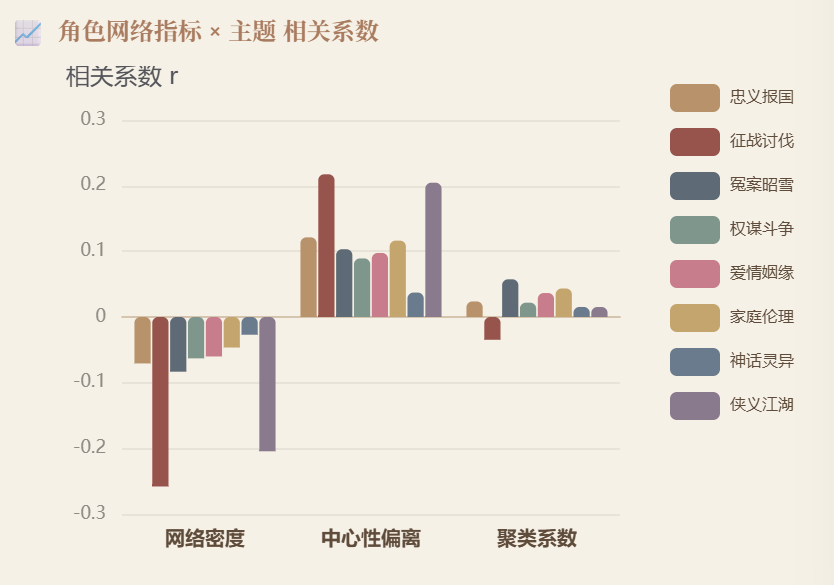
\includegraphics[width=0.7\textwidth]{Image/q5-2-rel-theme-causal-chart.png}
\caption{图5.1 角色网络指标与主题相关系数}
\end{figure}

{\fontsize{13bp}{18bp}\heiti\bfseries 5.3 主题簇与叙事组织偏好}

\vspace{4pt}
{\fontsize{12bp}{20bp}\kaishu
主题簇与叙事类型之间的卡方检验显著（\ensuremath{\chi^2}=84.61，\textit{df}=35，p=0.000005；关联强度 Cramér's V=0.107），说明主题不会完全决定叙事，但确实会改变叙事偏好。标准化残差最大的三组对应关系是：
}

{\fontsize{12bp}{20bp}\kaishu
\begin{enumerate}[leftmargin=2.2em,itemsep=2pt,topsep=2pt]
\item \textbf{“宫廷朝堂 + 家庭伦理 + 征战讨伐”更偏回环照应式}：标准化残差为 3.2，观测值 67，高于期望值 46，说明这类题材常用首尾照应来完成朝局与人伦的统一收束。
\item \textbf{“征战讨伐 + 家庭伦理 + 智谋韬略等”更偏悬念突转式}：标准化残差为 3.2，观测值 31，高于期望值 18，说明谋略和战事主题更依赖关键节点的突然抬升。
\item \textbf{同一主题簇也更偏三叠反复式}：标准化残差为 2.2，观测值 14，高于期望值 8，说明战事推进和谋局展开常借助重复升级来积累张力。
\end{enumerate}
}

\vspace{6pt}

{\fontsize{12bp}{20bp}\kaishu
从这组对应关系可以看出，我们更倾向于把主题结构理解为“更适合用什么节奏和组织方式来讲这个故事”，而不是简单决定“讲不讲这个故事”。
}

\vspace{6pt}

% ================= 图5.2：主题→叙事因果图 =================
% 文件存放位置：Image/q5-3-theme-narr-causal-chart.png
% 图片内容：任务五页面右侧“因果分析”面板中，选择“主题→叙事”，截取下方“主题簇 × 叙事类型正残差”图表
% 使用方法：图片准备好后，取消下方 figure 注释即可
% 操作步骤：
% 1. 保持任务五右侧“因果分析”面板打开；
% 2. 点击“主题→叙事”；
% 3. 截取下方堆叠条形图/残差图；
% 截图要求：保留图例和横纵标签，保证不同叙事类型颜色清晰可辨；不要截上方整段发现卡片，避免画面过满
%
\begin{figure}[H]
\centering
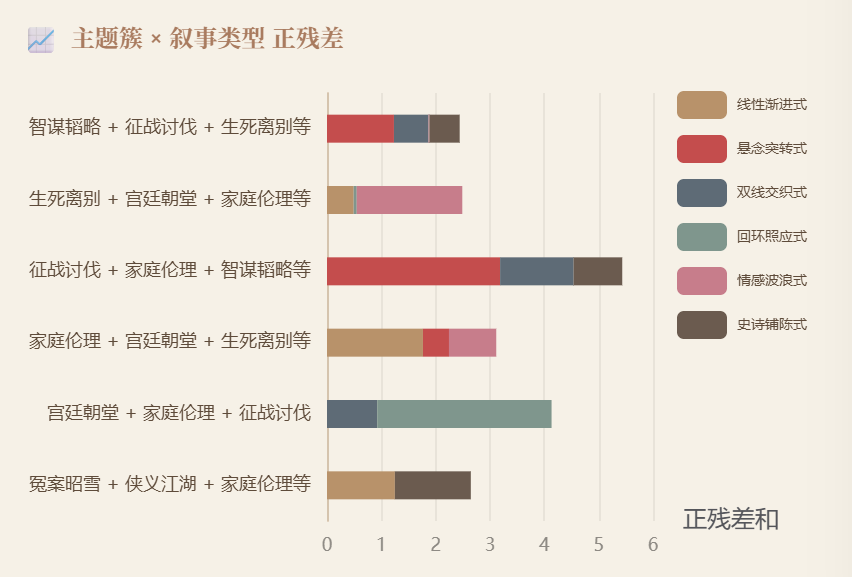
\includegraphics[width=0.7\textwidth]{Image/q5-3-theme-narr-causal-chart.png}
\caption{图5.2 主题簇与叙事类型的正残差分布}
\end{figure}

{\fontsize{13bp}{18bp}\heiti\bfseries 5.4 叙事类型与网络形态差异}

\vspace{4pt}

{\fontsize{12bp}{20bp}\kaishu
从 Kruskal-Wallis $H$ 检验看，8 类叙事在网络密度、中心性偏离和聚类系数上都存在显著差异（$H=734.39$、782.16、272.26，均 $p<0.001$），说明叙事方式会反过来塑造人物关系的呈现形态：
}

{\fontsize{12bp}{20bp}\kaishu
\begin{itemize}[leftmargin=2.2em,itemsep=2pt,topsep=2pt]
\item \textbf{回环照应式更紧密}：其平均网络密度最高（0.857），而史诗铺陈式最低（0.311），说明闭环叙事更容易把人物维持在高连接的近距离网络里。
\item \textbf{史诗铺陈式更单核}：其平均中心性偏离最高（2.195），而回环照应式最低（0.282），说明长篇铺陈往往需要少数核心人物调度更大的角色群。
\item \textbf{情感波浪式更团簇}：其平均聚类系数最高（0.851），而史诗铺陈式最低（0.791），说明情绪起伏型剧本更常围绕若干紧密小团体展开。
\end{itemize}
}

{\fontsize{12bp}{20bp}\kaishu
从这里我们还可以进一步看到，叙事方式不仅安排了冲突节奏，也会改变谁与谁更靠近、谁成为中心、谁被放在外围。
}

\vspace{6pt}

% ================= 图5.3：叙事→关系因果图 =================
% 文件存放位置：Image/q5-4-narr-rel-causal-chart.png
% 图片内容：任务五页面右侧“因果分析”面板中，选择“叙事→关系”，截取下方“各叙事类型的角色网络特征”图表
% 使用方法：图片准备好后，取消下方 figure 注释即可
% 操作步骤：
% 1. 保持任务五右侧“因果分析”面板打开；
% 2. 点击“叙事→关系”；
% 3. 截取下方分组柱图；
% 截图要求：优先保证“回环照应式”“史诗铺陈式”“情感波浪式”等关键标签清楚；如果横轴太密，可略微放大浏览器后再截
%
\begin{figure}[H]
\centering
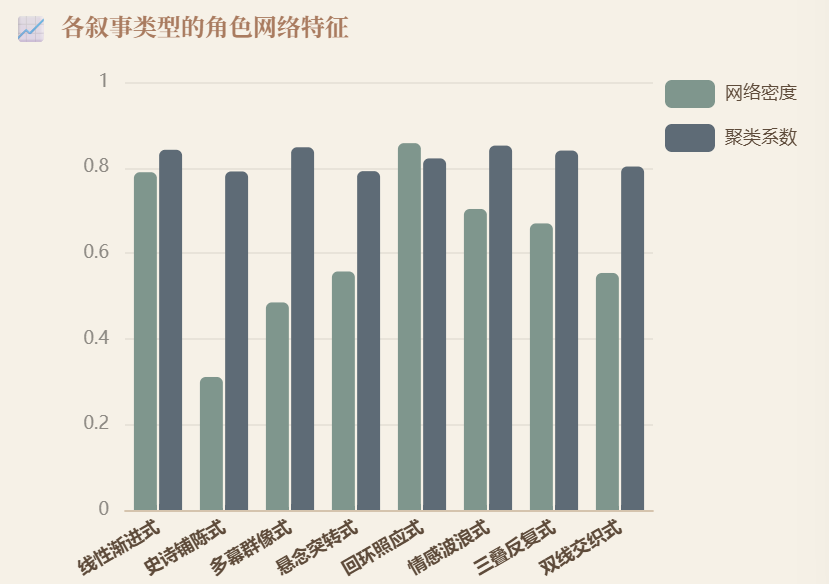
\includegraphics[width=0.7\textwidth]{Image/q5-4-narr-rel-causal-chart.png}
\caption{图5.3 各叙事类型的角色网络特征}
\end{figure}

{\fontsize{13bp}{18bp}\heiti\bfseries 5.5 六类综合结构原型及其落点}

\vspace{4pt}

{\fontsize{10.5bp}{15bp}\selectfont
\renewcommand{\arraystretch}{1.23}
\begin{center}
\begin{tabular}{C{0.22\textwidth} C{0.10\textwidth} L{0.24\textwidth} L{0.20\textwidth}}
\toprule
原型 & 数量 & 主导特征 & 常见组合 \tabularnewline
\midrule
低密度冤案昭雪型 & 439 & 角色较多、关系疏松 & 历史戏，偏史诗铺陈式 \tabularnewline
高聚类宫廷朝堂型 & 335 & 小团体闭合度高 & 历史戏，偏回环照应式 \tabularnewline
高聚类冤案昭雪型 & 328 & 关系紧密、规模较小 & 家庭戏，偏线性渐进式 \tabularnewline
强中心宫廷朝堂型 & 170 & 单核最强、群像规模大 & 历史戏，偏史诗铺陈式 \tabularnewline
均衡征战讨伐型 & 138 & 三类指标相对均衡 & 历史戏，偏悬念突转式 \tabularnewline
均衡冤案昭雪型 & 63 & 角色最少、结构极简 & 爱情戏，偏线性渐进式 \tabularnewline
\bottomrule
\end{tabular}
\end{center}
}

{\fontsize{12bp}{20bp}\kaishu
这说明 1{,}473 部剧本虽然题材各异，但角色关系、主题结构与叙事方式并不会无限分散，而会收敛成有限的结构家族。在交互系统中，还可以继续用“原型”筛选和星图详情把这些类型落回到具体剧本，并结合单剧面板查看其角色数量、关系边数、主题标签和结构指纹。
}

% \vspace{6pt}

% ================= 图5.4：结构原型星图拼图 =================
% 文件存放位置：Image/q5-5-prototype-starmap-collage.png
% 图片内容：建议使用 1 张拼图。左图截取任务五星图页面，打开左下“原型”筛选，选中 1--2 个结构原型，展示对应星体的空间分布；右图点击一部代表剧本，保留右侧详情面板中的角色关系条、表演形式条、主题标签和结构指纹
% 使用方法：图片准备好后，取消下方 figure 注释即可
% 操作步骤：
% 1. 在任务五星图页面左下角点击“原型”标签；
% 2. 选中 1--2 个结构原型，让星图中只高亮对应剧本，截取左图；
% 3. 再点击其中一颗代表性星体，右侧会弹出详情面板；
% 4. 截取详情面板中图形化最强的部分，优先保留角色关系条、表演形式条、主题标签和结构指纹；
% 截图要求：左图以星图空间分布和筛选芯片为主，右图以图形化模块为主；不要截“分析报告”文字；若右侧面板太长，可只裁图形部分，不必全截
%
\begin{figure}[H]
\centering
\includegraphics[width=1.0\textwidth]{Image/q5-5-prototype-starmap-collage.png}
\caption{图5.4 六类结构原型在星图中的分布及其单剧散落点}
\end{figure}

{\fontsize{13bp}{18bp}\heiti\bfseries 5.6 综合判断}

% \vspace{4pt}

{\fontsize{12bp}{20bp}\kaishu
综合来看，我们认为角色关系会影响主题能装下多大的世界，主题结构会影响叙事更偏向闭环收束、突转推进还是反复升级，叙事方式又会反过来改变网络的疏密、中心和团簇形态。三者并不是彼此孤立的三个结果，而是会进一步汇聚成若干可解释的对应关系和 6 类结构原型，呈现出稳定、可重复识别的整体结构类型。
}

% \vspace{5pt}

% ============================================================
% 总结
% ============================================================

{\fontsize{14bp}{22bp}\heiti\bfseries 总结}

% \vspace{4pt}

{\fontsize{12bp}{20bp}\kaishu
综合五个问题的分析，我们认为京剧剧本可以在“行当—关系—主题—叙事—综合关联”五个层面上形成一条彼此印证的证据链：角色—行当关系总体稳定而有弹性，不同剧目会形成不同的关系网络结构，主题表达既有跨类型共享的基础层，也有较清晰的组合原型，叙事高潮整体偏前，并在长篇剧目中表现出更早建峰的倾向，还可以进一步归纳为 8 类稳定模式；在此基础上，角色关系、主题结构与叙事方式之间还存在可以被量化检验、被图表验证的稳定关联，并最终收敛为 6 类结构原型。也正因为如此，1{,}473 部京剧剧本并不是彼此孤立的文本样本，而是一个具有稳定结构规律、类型差异和个案证据的多维文化系统；而“梨园万象”所做的，就是把这些总体规律、跨剧本比较和单剧验证都连接到了同一套可交互分析系统中。
}

\end{document}
